% \documentclass[10pt,landscape]{book} 
\documentclass[12pt ]{book}
%{report}
\usepackage[utf8]{inputenc}
\usepackage{amsmath,amsfonts,amssymb,euscript,dcolumn,mathbbol}
\usepackage[russian]{babel}
\usepackage{graphicx} 
%\textwidth  220mm%109mm  % 170mm    ДЛЯ ПРЕЗЕНТАЦИИ
%\textheight 130mm%108mm%240mm  %240/12     ДЛЯ ПРЕЗЕНТАЦИИ
%\textwidth  109mm%109mm  % 170mm    %A5
%\textheight 162mm%240mm  %240/12    %A5

\textwidth    170mm    %A4
\textheight   240mm    %A4
%\hsize=  170truemm
\topmargin -16mm
%\oddsidemargin -1.8cm % this for the A5 printer
%\evensidemargin -1.8cm
% this for the A5 printer
\oddsidemargin -0.4cm % this for the A5 printer
\evensidemargin -0.4cm


%\renewcommand{\contentsname}{Оглавление}\contentsname
\makeatletter
\newcommand{\l@abcd}[2]{\hbox to \textwidth{#1 {\huge\dotfill} #2}}
\newcommand{\l@Myabcd}[2]{\hbox to \textwidth{ #1 \leaders\hbox{~ }\hfil  }}
%%%%%%%%%%%%%%%%%%%%%%%%%%%%%%%%%%%%%%%%%%%%%%%%%%%%%%%%%%%%%%%%%%%%%%%%%%
\renewcommand{\l@chapter}[2] %Начало макроопределения (***глава в оглавлении***)
{\pagebreak[3] \vspace{1em plus 1pt}%
  \@tempdima=4.5em% место для номера главы (1.5em в стандарте)
  %\@pnumwidth=2em
    {% Дальше внутри группы...
   \rightskip=\@pnumwidth
   \leftskip=\@tempdima
   \bf
   \noindent
   \hspace{-\leftskip}% с левого поля
    #1 %\nolinebreak
   %\leaders\hbox to 0.5em {\hss. \hss }
\hfill
%\nolinebreak
    \rlap{\makebox[\@pnumwidth][r]{#2}}\par
    \nopagebreak[3]
   } %конец группы.
}% конец макроопределения
 
%%%%%%%%%%%%%%%%%%%%%%%%%%%%%%%%%%%%%%%%%%%%%%%%%%%%%%%%%%%%%%%%%%%%%%%%%%%%
\renewcommand{\@makechapterhead}[1]{ %Начало макроопределения (***для главы***)
 \vspace*{40pt} %Пустое место вверху страницы
 {\parindent=0pt
  \raggedright\Large\bf
  %\@chapapp{} %\@chapapp печатает слово"Глава"(см. ниже)
 {\Huge \bf Глава \arabic{chapter} }   %  \par  % чтобы номер главы - в отдельной строке
  \vspace{20pt} % между словом "Глава"и её заголовком
 \par
\Huge \bf #1
%\begin{centerline} #1  \end{centerline}   \centerline
%#1
\par % заголовок главы
  \nopagebreak %чтоб не оторвать заголовок от текста
  \vspace{40pt} % между заголовком и текстом
 } %конец группы.
}% конец макроопределения
%%%%%%%%%%%%%%%%%%%%%%%%%%%%%%%%%%%%%%%%%%%%%%%%%%%%%%%%%%%%%%%%%%%%%%%%%%
\renewcommand{\section}{\@startsection{section} %(***для раздела***)
 {1} %уровень вложенности раздела
 {0mm} %отступ от левого поля
 {3.5ex plus 1ex minus 2.ex } %вертикальный отступ До
 {2.3ex plus 0.2ex } %вертикальный отступ После
 {  \Large \bfseries
%\centerline
}% стиль
}% конец
%%%%%%%%%%%%%%%%%%%%%%%%%%%%%%%%%%%%%%%%%%%%%%%%%%%%%%%%%%%%%%%%%%%%%%%%%%
\def\Nthechapter{\arabic{chapter}}
\renewcommand{\@begintheorem}[2]{\begin{trivlist}\it
             \item[\hspace{\labelsep}{\bf #1\ #2.}]}
\renewcommand{\@biblabel}[1]{#1.\hfill}
%\renewcommand{\thechapter}{{\bf {Глава} \arabic{chapter}.   }}
\renewcommand{\thechapter}{{\arabic{chapter}}}
\renewcommand{\thesection}{\arabic{chapter}.\arabic{section}.}
\renewcommand{\thesubsection}{\arabic{chapter}.\arabic{section}.\arabic{subsection}.}
\renewcommand{\thesubsubsection}
             {\arabic{chapter}.\arabic{section}.\arabic{subsection}.\arabic{section}.}
%%%%%%%%%%%%%%%%%%%%%%%%%%%%%%%%%%%%%%%%%%%%%%%%%%%%%%%%%%%%%%%%%%%%%%%%%%%%%%%%%
%\renewcommand{\subsection}{\@startsection{subsection} %(***для подраздела***)
% {1} %уровень вложенности раздела
% {0mm} %отступ от левого поля
% {3.5ex plus 1ex minus 2.ex } %вертикальный отступ До
% {2.3ex plus 0.2ex } %вертикальный отступ После
% {  \large \bfseries   }% стиль
%}% конец
%%%%%%%%%%%%%%%%%%%%%%%%%%%%%%%%%%%%%%%%%%%%%%%%%%%%%%%%%%%%%%%%%%%%%%%%%%%%%%%%%
%\renewcommand{\subsubsection}{\@startsection{subsubsection} %(***для подподраздела***)
% {1} %уровень вложенности раздела
% {0mm} %отступ от левого поля
% {3.5ex plus 1ex minus 2.ex } %вертикальный отступ До
% {2.3ex plus 0.2ex } %вертикальный отступ После
% {  \bfseries   }% стиль
%}% конец

%\renewcommand{\@begintheorem}[2]{\begin{trivlist}\it
%             \item[\hspace{\labelsep}{\bf #1\ #2.}]}
%\newtheorem {lemma} {\bf Лемма}
%\newtheorem {theorem} {\bf Теорема}
%\newtheorem {corollary} {\bf Следствие}
%\newtheorem {proposal} {\bf Предложение}
%\newtheorem {definition} {\bf Определение}


\makeatother

\newcounter{ctheorem}[chapter]
\newcounter{clemma}[chapter]
\newcounter{cproposal}[chapter]
\newcounter{cdefinition}[chapter]
\newcounter{ccorollary}[chapter]

\def\theorem{\par \smallskip %\noindent
     \refstepcounter{ctheorem}
    {\bf  Теорема \arabic{chapter}.\arabic{ctheorem}.\ } \begin{it} }
\def\lemma{\par\smallskip %\noindent
     \refstepcounter{clemma}
    {\bf  Лемма \arabic{chapter}.\arabic{clemma}.\ } \begin{it} }
\def\proposal{\par\smallskip %\noindent
     \refstepcounter{cproposal}
    {\bf  Предложение \arabic{chapter}.\arabic{cproposal}.\ } \begin{it} }
\def\definition{\par\smallskip %\noindent
    \refstepcounter{cdefinition}
    {\bf  Определение \arabic{chapter}.\arabic{cdefinition}.\ } \begin{it} }
\def\corollary{\par\smallskip %\noindent
    \refstepcounter{ccorollary}
    {\bf  Следствие \arabic{chapter}.\arabic{ccorollary}.\ } \begin{it} }

\def\endtheorem{\end{it}\par\smallskip}
\def\endlemma{\end{it}\par\smallskip}
\def\endproposal{\end{it}\par\smallskip}
\def\enddefinition{\end{it}\par\smallskip}
\def\endcorollary{\end{it}\par\smallskip}

\newcommand{\ex}[2]{Результат выполнения: \\ in: #1 \\ out: #2}
\newcommand{\comm}[2]{$\backslash {\mathbf {#1}} #2$}
\begin{document}

\sloppy




\renewcommand{\theequation}{\arabic{chapter}.\arabic{equation}}

%счетчик для примеров
\newcounter{examplec}
\setcounter{examplec}{0}
\newcommand{\example}[1]{\addtocounter{examplec}{1}\null\underline{\textbf{Пример \arabic{examplec}}. #1} }


\newcounter{tablec}
\setcounter{tablec}{0}
\newcommand{\mytable}[1]{\addtocounter{tablec}{1}{\begin{flushright}Таблица \arabic{tablec}\end{flushright}}\textbf{ #1}} 


%\hsize=  170truemm
\def\refname{{\centerline{\Large{ЛИТЕРАТУРА}}}}%
%\def\bibname{{\centerline{\normalsize{ЛИТЕРАТУРА}}}}%
\def\bibname{{\centerline{\Large{ЛИТЕРАТУРА}}}}%
\def\abstractname{{{ \  }}}%Аннотация
\def\chaptername{ \hspace{200pt} \Large  Глава}%
\def\appendixname{Приложение}%
\def\contentsname{\centerline{\Large{ОГЛАВЛЕНИЕ}}}%
\def\listfigurename{Список рисунков}%
\def\listtablename{Список таблиц}%
\def\indexname{Индекс}%
\def\figurename{Рисунок}%
\def\tablename{Таблица}%
\def\partname{Часть}%
\def\enclname{прилагается}%
\def\ccname{копии}%
\def\headtoname{Кому}%
\def\pagename{Стр.}
\pagestyle{plain}



\newcommand{\diag}{{\mathrm{diag}}}
\newcommand{\sign}{{\mathrm{sign}}}
\newcommand{\Nr}{\,{\mathrm{Nr}}\,}
\newcommand{\rank}{{\mathrm{rank}}}
\newcommand{\ce}{\centerline}
\newcommand{\e}{{\mathbf e}}
\newcommand{\tb}{ \tilde{b}}
\newcommand{\tB}{ \tilde{B}}
\newcommand{\tD}{ \tilde{D}}
\newcommand{\tA}{ \tilde{A}}
\newcommand{\tF}{ \tilde{F}}
\newcommand{\tx}{ \tilde{x}}
\newcommand{\hbx}{{\hat{\mathbf x}}}
\newcommand{\bx}{{\mathbf x}}
\newcommand{\bZ}{{\mathbb Z}}

\def\head#1{\vskip6pt{\bf #1}}
\newcommand{\intt}{{\bf int }}

\newcommand{\ra}{\rangle}
\newcommand{\la}{\langle}
\newcommand{\ul}{\Large \bf  \underline }
\newcommand{\tchi}{{\tilde{\mathbf \chi}}}
\newcommand{\mtr}[4]%
{\left(\begin{array}{cc}#1 & #2\\#3 & #4\end{array}\right)}
\newcommand{\Dmtr}[4]%
{\left|\begin{array}{rr}#1 & #2\\#3 & #4\end{array}\right|}
\newcommand{\mtrk}[4]%
{\left[\begin{array}{cc}#1 & #2\\#3 & #4\end{array}\right]}

\newcommand{\mtrc}[2]%
{\left(\begin{array}{c}#1 \\#2 \end{array}\right)}
\newcommand{\mtrs}[2]%
{\left[\begin{array}{c}#1 \\#2 \end{array}\right]}
\newcommand{\LCM}{{\mathrm{LCM}}}  \newcommand{\R}{{\bf R}}
\date {}
\newcommand{\tsec}[1]{\bigskip \centerline{\normalsize {#1}}\bigskip \par}
\newcommand{\ttsec}[2]{\bigskip {\centerline{\normalsize {#1}}}\par\noindent
{\centerline{\normalsize {#2}}} \bigskip}
\newcommand{\tttsec}[3]{\bigskip {\centerline{\normalsize {#1}}}
\par\noindent
{\centerline{\normalsize {#2}}} \par\noindent
{\centerline{\normalsize {#3}}} \bigskip}
\newcommand{\tsub}[1]{{\medskip \bf {#1}}\par}


%\pageno=1
%\magnification \magstep2

% Я \hoffset=30truemm
% Я \voffset=20truemm
\frenchspacing
%\NoRunningHeads
%\TagsOnRight
%\LimitsOnInts
%\LimitsOnSums
%\widowpenalty=150 % было 10000
%\clubpenalty=150  % было 10000
%\binoppenalty=150
%\relpenalty=150



\def\endd{\vfill\eject}
\def\Beta{\roman B}

\let\eps\varepsilon
\def\const{\operatorname{const}}
\def\R{{\Bbb R}}
\def\K{{\Bbb K}}
\def\N{{\Bbb N}}
\def\Z{{\Bbb Z}}
\def\al{\alpha}
\def\be{\beta}
\def\beF{\widehat{\bf \beta}}
\def\alF{\widehat{\bf \alpha}}
\def\de{\delta}
\def\deF{\widehat{\bf \delta}}
\def\si{\sigma}
\def\siF{\widehat{\bf \sigma}}
\def\di{{\bf {\rm diag}}}
\def\G{\Gamma}
\def\L{\Lambda}

\def\cA{{\bf \mathcal A}}
\def\cC{{\bf \mathcal C}}
\def\cD{{\bf \mathcal D}}
\def\cG{{\bf \mathcal G}}
\def\cH{{\bf \mathcal H}}
\def\cL{{\bf \mathcal L}}
\def\cK{{\bf \mathcal K}}
\def\cM{{\bf \mathcal M}}
\def\cT{{\bf \mathcal T}}
\def\cS{{\bf \mathcal S}}
\def\cU{{\bf \mathcal U}}
\def\cY{{\bf \mathcal Y}}
\def\cZ{{\bf \mathcal Z}}


\def\cAF{{\widehat {\bf \cal A}}}
\def\cGF{{\widehat {\bf \cal G}}}
\def\cFF{{\widehat {\bf \cal F}}}
\def\cHF{{\widehat {\bf \cal H}}}
\def\cLF{{\widehat {\bf \cal L}}}
\def\cMF{{\widehat {\bf \cal M}}}
\def\cVF{{\widehat {\bf \cal V}}}
\def\cUF{{\widehat {\bf \cal U}}}
\newcommand{\bR}{{\mathbf R}}
\newcommand{\bL}{{\mathbf L}}
\newcommand{\bM}{{\mathbf M}}
\newcommand{\bU}{{\mathbf U}}
\newcommand{\bA}{{\mathbf A}}
\newcommand{\bB}{{\mathbf B}}
\newcommand{\bC}{{\mathbf C}}
\newcommand{\bD}{{\mathbf D}}
\newcommand{\bF}{{\mathbf F}}
\newcommand{\bE}{{\mathbf E}}
\newcommand{\bG}{{\mathbf G}}
\newcommand{\bW}{{\mathbf W}}
\def\ba{{\mathbf a}}
\def\bp{{\mathbf p}}
\def\bq{{\mathbf q}}
\def\br{{\mathbf r}}
\def\bK{{\mathbf K}}
\def\leq{\leqslant }
\def\geq{\geqslant }
\def\tF{\widetilde{F}}
\def\tG{\widetilde{G}}
\def\tL{\widetilde{L}}
\def\tl{\widetilde{\ell}}
\def\tM{\widetilde{M}}
\def\tU{\widetilde{U}}
\def\tV{\widetilde{V}}
\def\tW{\widetilde{W}}
\def\tu{\widetilde{u}}
\def\btL{\widetilde{\mathbf {\rm L}}}
\def\btU{\widetilde{\mathbf {\rm U}}}
%_________________
\def\tcF{\widetilde{\cal F}}
\def\tcL{\widetilde{\cal L}}
\def\tcM{\widetilde{\cal M}}
\def\tcU{\widetilde{\cal U}}
\def\Ann{\rm {Ann \,}}
\def\GI{\rm {GI \,}}
\def\Frac{\rm {Frac \,}}
\def\GCD{\rm {НОД \,}}

\let\bs\textbackslash

\thispagestyle{empty}
\begin{LARGE}
\
\bf{
\centerline{  }
 

 
\centerline{Руководство по языку}
\centerline{}
 

\centerline{}
\centerline{<<MATHPAR>>}
}
 
\end{LARGE}

\bigskip
\
 \bigskip

\bigskip
\centerline{ВЕРСИЯ 6.00}

\bigskip
\
 \bigskip

\bigskip
\
\bigskip
 

\vfill
\ce{  10.02.2016  }
\tableofcontents
\vfill

\eject 

 
\chapter{Введение}
Данное руководство по языку Mathpar поможет Вам при решении математических задач. 
Оно будет всегда Вашим помощником, когда Вам нужно воспользоваться математикой:
будь то решение задачи в школе или в университете, выполнение научных расчетов или решение производственной задачи.

Mathpar поможет Вам делать простые числовые или алгебраические операции, строить графики кривых и поверхностей.

Он поможет Вам решать задачи различных разделов математического анализа, алгебры, геометрии, задачи по физике, по химии и другие.  

Если же Вы профессионально применяете математику, то он поможет Вам избавиться от рутинных вычислений и оперировать с очень большими математическими объектами, задействуя при этом суперкомпьютеры. 
Mathpar позволяет оперировать с функциями и функциональными матрицами, получать как точные численно-аналитические решения, так и решения, в которых числовые коэффициенты получаются с требуемой степень точности.

В основе языка Mathpar лежит широко используемый математиками  и физиками язык ТеХ, который обычно используют для набора математических текстов.

Вы можете сохранить как постановку задачи, так и ход ее решения. При этом можете сохранять и текстовый вид (Mathpar, TeX или MathML) и изображение (pdf, jpg).

Весь излагаемый тут материал делится на 14 глав.

Для первого знакомства достаточно ознакомиться с двумя следующими главами данного руководства. 

Во второй главе описывается ввод данных и выполнение простейших вычислений. 
Даются обозначения для элементарных функций, таких как логарифм, синус, косинус и т.д., 
и констант --- $\pi$, $e$, $i$, а также констант, которые необходимы для задания числовых множеств. 
Описываются способы задания векторов и матриц, арифметические операции над ними, команды генерации случайных чисел, полиномов и матриц, команды для решения алгебраических уравнений. 
Для всех команд приведены примеры.

Третья глава посвящена построению графиков функций. Mathpar позволяет строить графики функций, которые заданны явно или параметрически,
кроме того функции могут быть заданы таблично -- множеством значений функций на конечном множестве значений аргумента. 
Можно выполнить построение нескольких графиков в одной системе координат. 

В четвертой главе описываются способы задания окружения в системе Mathpar, т.е. того пространства, 
в котором будут определяться математические объекты. 
В любой момент Вы можете сменить окружение и задать новое алгебраическое пространство.  

В пятой главе описаны команды для задания математических функций одной или нескольких переменных, их композиций, вычисления значений функции в точке, подстановки выражений в функции, вычисление предела функции в точке, символьного интегрирования композиций элементарных функций. Приводятся примеры выполнения   команд. 

Шестая глава посвящена действиям с рядами. Рассматриваются способы задания ряда. Даются команды для сложения, вычитания, умножения двух рядов и для разложения функции в ряд Тейлора с определенным количеством членов ряда. 

В седьмой главе описаны команды для решения обыкновенных дифференциальных уравнений и систем, а также   дифференциальных уравнений с частными производными.

Восьмая глава посвящена полиномиальным вычислениям. Рассматриваются команды для вычисления значения полинома в точке, суммирования полинома по переменным, вычисления базиса Гребнера полиномиального идеала над рациональными числами. 

В девятой главе описываются матричные функции --- вычисление транспонированной матрицы, определителя матрицы, присоединенной и обратной матриц, эшелонной формы матрицы, ядра оператора, характеристического полинома матрицы и другие.

Десятая глава посвящена функциям теории вероятностей и математической статистики. Описывается задание дискретной случайной величины,  команды для вычисления математического ожидания дискретной случайной величины, дисперсии, среднего квадратичного отклонения, суммы, произведения двух дискретных случайных величин, коэффициента ковариации, коэффициента корреляции, построения многоугольника распределения и функции распределения дискретной случайной величины. В этой главе рассматриваются команды для задания выборок и для вычисления функций для них: выборочное среднее, выборочная дисперсия, коэффициент ковариации  и коэффициент корреляции для двух выборoк.

Mathpar не только активный математический язык, но он еще и процедурный язык программирования.
Одиннадцатая глава посвящена программированию в языке Mathpar. В этой главе описаны правила записи процедур и основной части программы,  правила записи операторов ветвления и цикла.  Вы можете написать программу, содержащую Ваши новые процедуры и функции, и потом много раз использовать эти процедуры и функции для выполнения необходимых Вам вычислений. Mathpar можно использовать для обучения программированию в школе.

В главе двенадцатой описываются команды, которые управляют вычислениями на суперкомпьютере.
Для решения вычислительных задач, которые требуют большого времени вычислений или больших объемов памяти, разработаны специальные функции, которые предоставляют Вам ресурсы 
суперкомпьютера. При использовании этих функций вычисления производятся не на одном процессоре, а на выделенном множестве ядер суперкомпьютера, количество которых заказывает пользователь.
Это такие операции, как вычисление базиса Гребнера, присоединенной матрицы,  ступенчатого вида матрицы, обратной матрицы, определителя,  ядра линейного оператора,  характеристического полинома и др. 
На момент подготовки этой редакции руководства пользователя вычисления  на суперкомпьютере не поддерживаются.

В тринадцатой главе приведен список основных операторов в языке Mathpar.

В четырнадцатой главе приведены примеры решения задач по физике.
\chapter{Знакомство и первые шаги}
Эта глава посвящена первому знакомству с возможностями, которые Вам открывает Mathpar.
Язык Mathpar, который описывается ниже, может рассматриваться, как некоторое развитие языка TeX.
Язык TeX предназначен для записи математических текстов и подготовке их к публикации.
Его можно считать пассивным по сравнению с языком Mathpar, который позволяет делать вычисления,
то есть является активным языком математики. Как формулировка задачи,
так и результаты вычислений, записываются на языке Mathpar.

Сразу после вычислений Вы видите весь математический текст в виде pdf-изображения,
в том виде, как принято представлять математическую запись в научных и технических публикациях.

Этот результат может быть использован дальше несколькими способами.
 
(1) Можно кликнуть по тексту мышкой, и он вернется к исходному виду языка Mathpar.
Есть и другой способ переключения изображения текста: при помощи кнопки%begindelete
<<
\includegraphics[scale=0.6]{pictures/button_arrows.png}>>%enddelete
, расположенной между кнопками <<$\blacktriangleright$>> и <<$+$>>.

(2) Можно кликнуть по {\bf изображению математической записи} правой кнопкой мышки.
В этом случае появится выпадающее меню. Верхнее поле <<Show Math As>> позволяет
перейти к выбору  языка вывода. Предлагается выбрать TeX или MathML.
И затем открыть поле с желаемым текстом.

Например, матрица A, размера $2\times 2$, в Mathpar будет записана так:

A=[[a, b], [c, d]];

в TeX она выглядит так:

A= $\backslash$left(\comm{begin}{\{array\}}\{${cc}$\}$ a \& b$ $\backslash\backslash c \& d \backslash\backslash$ \comm{end}{\{array\}}$\backslash$right).

В MathML это еще более громоздкое выражение.
 
Полученный текст на языке TeX или MathML можно скопировать и поместить  в TeX- 
или html-файл и использовать для публикации. Кроме того, можно получить обычное 
изображение и разместить его в любом документе. Это необходимо, например, 
когда требуется сохранить график функции или решение задачи.


\section{Ввод данных,  решение задачи}

В  центральной части экрана находится поле ввода. Здесь Вы размещаете математические выражения.  
Для решения задачи надо нажать на кнопку <<${\blacktriangleright}$>>, которая 
расположена над полем ввода. Кроме того, можно использовать сочетание клавиш {\it Ctrl+Enter}. 
Например, можно набрать 2+2 и нажать <<$\blacktriangleright$>>.

В верхней части экрана находятся активные поля $\fbox{Помощь}$ и $\fbox{Руководство}$. 
Указывая мышкой на эти поля, Вы можете перейти к страницам Помощи или открыть Руководство по языку Mathpar.

%begindelete
На рисунке приведен пример простого задания.  
 
 \begin{figure}
 \label{1_1}
\begin{center}
   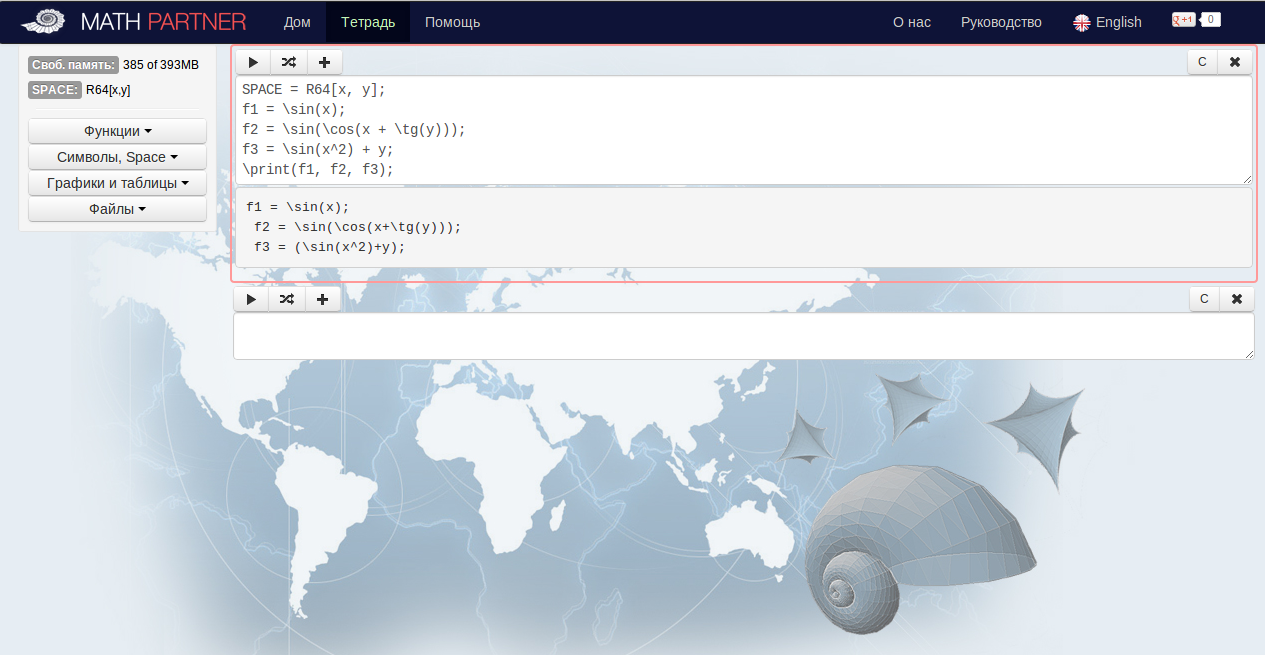
\includegraphics[scale=0.5]{pictures/1_1}
\end{center}
 \caption{Запись задания в поле ввода}
 \end{figure}
%enddelete

На страницах Помощи все поля с примерами являются активными полями, 
содержащиеся там задачи можно тут же решить и увидеть ответ.  
Для этого  нужно кликнуть по кнопке <<$\blacktriangleright$>> или же можно 
поставить курсор на поле примера и нажать {\it Ctrl+Enter}. 
Можно копировать текст из любого примера и перенести его в Ваше основное поле ввода. 
Для этого можно использовать выделение текста мышкой, копирование и вставку этого текста 
с помощью сочетания клавиш {\it Ctrl+С} и {\it Ctrl+V}, соответственно, для копирования и вставки.

Текст, который Вы можете вводить в поле ввода, состоит из комментариев и математических операторов.

При вводе комментариев, то есть любого поясняющего текста, необходимо брать его в кавычки. 
Например: ($"$ это комментарий $"$). Кавычки разрешается использовать только для комментариев. 
В тексте комментариев можно использовать, например, такие кавычки  <<  >>. 
Когда в комментариях нужно иметь математическое выражение, как часть комментария, 
то его необходимо окаймить знаками доллара ($\$$). Например, можно написать такой комментарий: \\
$"$Два обозначения $\$ \backslash exp(x)\$$  и  $\$\backslash e  \widehat{\ }{} x\$$ 
применяются для экспоненциальной функции.$"$

При вводе математических выражений их необходимо разделять точкой с запятой (;) 
или текстом комментариев, которые заключены в кавычки. Можно не ставить 
точку с запятой после последнего оператора. В математических операторах, 
когда необходимо вставить текст, нужно использовать апострофы: ('текст в математическом операторе' ).

Для вывода результатов можно использовать команду \comm{print}{()}, 
где в качестве аргументов,  разделенных запятыми,  необходимо указать имена 
тех выражений, которые требуется вывести.  Если среди команд не встретился 
оператор печати \comm{print}{()} или какой-нибудь другой оператор вывода (\comm{plot}{()}, 
\comm{prints}{()} и т. д.), то будет выводится результат, полученный в последнем 
операторе или последней новой переменной.

Команды и операторы начинаются с символа <<back slash>> ($\backslash$). 

Кнопка $\fbox{+}$ предназначена для добавления полей ввода. Для удаления поля ввода 
можно воспользоваться сочетанием клавиш {\it Ctrl+Del} или крестиком  $\fbox{х}$, 
расположенным над полем ввода справа.  

Кнопка $\fbox{C}$, расположенная над полем ввода справа, предназначена 
для отмены всех введенных раннее обозначений.     
Отмена обозначений позволяет получать формулы, в которых стоят символы, а не числа.

В левой верхней части экрана находятся поля, в которых указано текущее окружение 
и объем оперативной памяти в мегабайтах. Окружение фиксируется числовым множеством 
и именами основных переменных. Под этим полем расположены различные меню, 
которые облегчают ввод функций и операторов.


\subsection{Работа с файлами}
Функции для работы с файлами доступны из раскрывающейся панели «Файлы», расположенной в меню слева.

Существуют следующие возможности для обработки файлов:

1) Сохранение последней выполненной секции в виде файла PDF с помощью
кнопки «Сохранить PDF». Можно указать собственный размер страницы (в сантиметрах),
по умолчанию указан размер А4 (21х29.7 см).

2) Загрузка текстовых файлов на сервер Mathpar с помощью кнопки «Загрузить файл».
Под этой кнопкой расположен список загруженных файлов. Файлы должны содержать выражения 
на языке Mathpar или таблицы в специальном формате.

Таблица состоит из строки с заголовком (произвольные строки) и строк с числами.
Столбцы отделяются знаком табуляции. Функции для работы с таблицами доступны 
в разделе «Графики и таблицы» (см. также раздел 3.1 Построение графиков функций 
системы помощи).

3) Ввод выражений на языке Mathpar из загруженного файла с помощью функции \comm{fromFile}{()}.
Например, создать выражение из загруженного файла myfile.txt и присвоить 
это выражение переменной $a$ можно командой a = \comm{fromFile}{('myfile.txt')}.


\section{Математические функции}
Приняты следующие обозначения для элементарных функций и констант.

\subsection{Константы}
\hspace*{4mm}  $\backslash$i --- мнимая единица,

$\backslash$e --- основание натурального логарифма,

$\backslash$pi --- число $\pi$,  то есть отношение длины окружности к диаметру,

$\backslash$infty -- знак бесконечности.


\subsection{Функции одного аргумента}

\hspace*{4mm} $\backslash$ln --- натуральный логарифм, 

 $\backslash$lg --- десятичный логарифм, 

 $\backslash$sin --- синус, 

 $\backslash$cos --- косинус, 

 $\backslash$tg --- тангенс, 

 $\backslash$ctg --- котангенс, 

 $\backslash$arcsin --- арксинус, 

 $\backslash$arccos --- арккосинус, 

 $\backslash$arctg --- арктангенс, 

 $\backslash$arcctg --- арккотангенс, 

 $\backslash$sh --- синус гиперболический, 

 $\backslash$ch --- косинус гиперболический, 

 $\backslash$th --- тангенс гиперболический, 

 $\backslash$cth --- котангенс гиперболический, 

 $\backslash$arcsh --- арксинус гиперболический, 

 $\backslash$arcch --- арккосинус гиперболический, 

 $\backslash$arcth --- арктангенс гиперболический, 

 $\backslash$arccth --- арккотангенс гиперболический, 

 $\backslash$exp --- экспонента, 

 $\backslash$sqrt --- корень квадратный, 

 $\backslash$abs --- абсолютное значение для действительных чисел,  модуль для комплексного числа,

 $\backslash$sign --- знак числа. Возвращает 1, 0,  -1,  когда число положительное, ноль или отрицательное,  соответственно,

 $\backslash$unitStep$(x)$ --- это функция, которая при $x\geqslant 0$ принимает значение $1$, а
при $x<0$ принимает значение $0$;

 $\backslash$fact --- факториал.  Определен для целых положительных чисел. Равносильная запись~--- <<n!>>.


\subsection{Функции двух аргументов}

\hspace*{4mm}  $\widehat{\ }{}$ --- степень,

 $\backslash$log --- логарифм от функции по указанному основанию,

 $\backslash$rootOf(x, n) --- корень степени n из x,   

 $\backslash$Gamma --- функция Гамма,

 $\backslash$Gamma2 --- функция Гамма 2,

 $\backslash$binomial --- число сочетаний. 


\smallskip

\underline{Примеры. }

\vspace*{-3mm}
\begin{verbatim}
SPACE = R64[x, y];
f1 = \sin(x);
f2 = \sin(\cos(x + \tg(y)));
f3 = \sin(x^2) + y;
\print(f1, f2, f3);
\end{verbatim}

%begindelete
\vspace*{-3mm}
Результат выполнения:\\
$SPACE=R64[x,y];$\\
$f1 = sin(x); $\\
$f2 = sin(cos(x+tg(y))); $\\
$f3 = sin(x^{2})+y. $
%enddelete


\section{Действия с функциями}

Для перечисленных выше функций и их композиций можно вычислить значение функции в точке,  подставить выражения в функцию вместо аргументов,  вычислить предел функции,  ее производную.  Для этого определены следующие команды. 

 
Для вычисления значения функции в точке необходимо выполнить команду \\
\comm{value}{(f, [var1, var2,\ldots, varn])}, 
где $f$~---  функция,  а $var1, var2, \ldots, varn$~--- значения соответствующих переменных кольца. 
 Для подстановки выражений в функцию необходимо выполнить команду \\
\comm{value}{(f, [func1, func2, \ldots,  funcn])},  где $f$~--- это функция,  
$func1, func2, \ldots,  funcn$~--- функции,  которые подставляются вместо соответствующих переменных. 

 Для вычисления предела функции в точке необходимо выполнить команду \\
\comm{lim}{(f, var)},  
где $f$~--- это  функция,  а $var$~--- точка,  в которой требуется найти предел. 

 Для вычисления производной функции $f$ по переменной $y$ из кольца $\mathbb{Z}[x,\ y,\ z]$
 необходимо выполнить команду  \comm{D}{(f, y)}.  Для нахождения смешанной производной первого порядка от функции $f$ существует команда 
\comm{D}{(f, [x, y])},  для нахождения производной высших порядков нужно использовать команду $\backslash {\mathbf {D}} (f, [x \widehat{\ }{} k, z \widehat{\ }{} m, y \widehat{\ }{} n])$,  где $k,  m,  n$ указывают,  какого порядка по соответствующей переменной вычисляется производная. 


\smallskip

\underline{Примеры. }

\vspace*{-2mm}
\begin{verbatim}
SPACE = R[x, y];
f = \sin(x^2 + \tg(y^3 + x));
g = \value(f, [1, 2]);
\print(g);
\end{verbatim}
%begindelete

\vspace*{-2mm}
Результат выполнения:\\
in: $SPACE=R[x, y];$\\ 
\hspace*{4mm} $f=sin(x^2+tg(y^3+x)); $\\
\hspace*{4mm} $g=value(f,\ [1,\ 2]); $\\
\hspace*{4mm} $print(g);$\\
out: $g = 0. 52;$\\
\vspace*{-2mm}
%enddelete

\begin{verbatim}
SPACE = Z[x, y];
f = x + y;
g = f^2;
r = \value(f, [x^2, y^2]);
\print(g, f, r);
\end{verbatim}
%begindelete

\vspace*{-2mm}
Результат выполнения: \\
in: $SPACE=Z[x, y]; $\\
\hspace*{4mm} $f=x+y;$\\ 
\hspace*{4mm} $g=f^2; $\\
\hspace*{4mm} $r=value(f, [x^2, y^2]); $\\
\hspace*{4mm} $print(g, f, r);$\\
out: $g = y^{2}+2yx+x^{2}; $ \\
\hspace*{4mm} $f = y+x;$ \\ 
\hspace*{4mm} $r=x^2+y^2 $
\vspace*{-3mm}
%enddelete

\begin{verbatim}
SPACE = R64[x];
f = \sin(x) / x;
g = \lim(f, 0);
\print(g);
\end{verbatim}
%begindelete

\vspace*{-3mm}
Результат выполнения: \\
in: $ SPACE=R64[x]; $\\
\hspace*{4mm} $f=sin(x)/x; $\\
\hspace*{4mm} $g=lim(f, 0); $\\
\hspace*{4mm} $print(g);$\\
out: $g = 1. 00;$
\vspace*{-3mm}
%enddelete

\begin{verbatim}
SPACE = Z[x, y];
f = \sin(x^2 + \tg(y^3 + x));
h = \D(f, y);
\print(h);
\end{verbatim}
%begindelete

\vspace*{-3mm}
Результат выполнения:\\
in: $SPACE=Z[x, y]; $\\
\hspace*{4mm} $f=sin(x^2+ tg(y^3+x)); $\\
\hspace*{4mm} $h= D(f, y);$\\ 
\hspace*{4mm} $print(h);$\\
out: $h = 3y^2 cos(x^2+tg(y^3+x))/(cos(y^3+x))^2;$
%enddelete

\section{Решение алгебраических уравнений}

Для решения алгебраических уравнений нужно выполнить команду \comm{solve}{}.  Ниже используется команда настройки окружения
<<FLOATPOS=N>>.  Она устанавливает число десятичных знаков после запятой $(N)$,  которые должны появиться при выводе числового результата приближенных вычислений.  Она не связана с процессом вычислений,  а только с выводом.  По умолчанию $FLOATPOS=2$. 

\underline{Примеры. }

\vspace*{-2mm}
\begin{verbatim}
SPACE = R64[x];
b = \solve(x^2 - 5x + 6 = 0);
\end{verbatim}
%begindelete

\ex{$SPACE=R64[x]; $\\
\hspace*{4mm} $b=solve(x^2-5x+6=0);$ }{$[2. 00, 3. 00];$}
%enddelete
 
\begin{verbatim}
SPACE = R64[x];
FLOATPOS = 6;
b = \solve(x^4 + 2x + 1 = 0);
\end{verbatim}
%begindelete

\ex{$SPACE=R64[x];$\\ 
\hspace*{4mm} $FLOATPOS=6; $\\
\hspace*{4mm} $b=solve(x^4 +2x +1=0);$}{$[-0.543689,-1.000000];$} 
%enddelete

\begin{verbatim}
SPACE = R64[x];
FLOATPOS = 0;
b = \solve(x^3 + 3x^2 + 3x + 1 = 0);
\end{verbatim}
%begindelete


\ex{$SPACE=R64[x]; $\\
\hspace*{4mm} $FLOATPOS=0;$\\
\hspace*{4mm} $b=solve(x^3+3x^2+3x+1=0);$}{$-1$.}
%enddelete


\section{Решение алгебраических неравенств}

Для решения алгебраических неравенств нужно выполнить команду \comm{solve}{}, в которой записано неравенство.
Можно решать строгие и не строгие алгебраические неравенства. Открытый интервал обозначается круглыми скобками ( ), а закрытый интервал -- квадратными скобками [ ], множество обозначается фигурными скобками \{ \}.


\begin{verbatim}
SPACE = R[x];
b = \solve(x^2-5x+6 < 0);
\end{verbatim}
%begindelete

\ex{$SPACE=R[x]; $\\
\hspace*{4mm} $b=solve(x^2-5x+6 < 0);$}{$(2,3)$.}
%enddelete

\begin{verbatim}
SPACE = R[x];
b = \solve((x+1)^2(x-3)(x+5) \ge 0);
\end{verbatim}
%begindelete

\ex{$SPACE=R[x]; $\\
\hspace*{4mm} $b=solve((x+1)^2(x-3)(x+5) \ge 0);$}{$(-\infty,-5] \cup{-1}\cup[3,\infty)$.}
%enddelete

\begin{verbatim}
SPACE = R[x];
b = \solve((x^2+11x+28)/(x+5) \le 0);
\end{verbatim}
%begindelete

\ex{$SPACE=R[x]; $\\
\hspace*{4mm} $b=solve((x^2+11x+28)/(x+5) \le 0);$}{$(-\infty,-7]\cup(-5,-4]$.}
%enddelete

\begin{verbatim}
SPACE = Q[x];
b = \solve(x^2 + 4x - 7 = 0);
\end{verbatim}
%begindelete

\ex{$SPACE=Q[x]; $\\
\hspace*{4mm} $b=solve((x^2 + 4x - 7 = 0);$}{$[(\sqrt{11}+(2)),(2-\sqrt{11})];$.}
%enddelete

\section{Решение систем алгебраических неравенств}

Для решения систем алгебраических неравенств нужно выполнить команду \comm{solve}{[In1, In2, ..., Ink]}, где $[In1, In2, ..., Ink]$~--- вектор неравенств.
Система может содержать строгие и не строгие алгебраические неравенства. Открытый интервал обозначается круглыми скобками ( ), а закрытый интервал~--- квадратными скобками [ ], множество обозначается фигурными скобками \{ \}.

\begin{verbatim}
SPACE = R[x];
b = \solve([x^2+4x-5 > 0, x^2-2x-8 < 0]);
\end{verbatim}
%begindelete

\ex{$SPACE=R[x]; $\\
\hspace*{4mm} $b=solve([x^2+4x-5 > 0, x^2-2x-8 < 0]);$}{$(1,4)$.}
%enddelete

\begin{verbatim}
SPACE = R[x];
b = \solve([x^2-x-6 \ge 0, x^2-4x-12 < 0]);
\end{verbatim}
%begindelete

\ex{$SPACE=R[x]; $\\
\hspace*{4mm} $b=solve([x^2-x-6 \ge 0, x^2-4x-12 < 0]);$}{$(-4,-2]\cup[3,4)$.}
%enddelete

\begin{verbatim}
SPACE = R[x];
b = \solve([x^2-4 < 0, x+1 > 0, 0.5-x > 0]);
\end{verbatim}
%begindelete

\ex{$SPACE=R[x]; $\\
\hspace*{4mm} $b=solve([x^2-4 < 0, x+1 > 0, 0.5-x > 0]);$}{$(-1,0.5)$.}
%enddelete

\section{Операции на подмножествах действительных чисел}

Подмножество, содержащее несколько интервалов можно задать так 
\comm{set}{((a,b),(c,d])} , где $a,b,c,d$~--- числа.
Здесь интервал обозначается круглыми скобками ( ), полуоткрытый интервал -- одной круглой и одной квадратной скобкой [ ) или ( ],
а отрезок --   квадратными скобками [ ]. Точка обозначается фигурными скобками \{ \} или как закрытый интервал.

Простые подмножества обозначаются такими же скобками, но перед каждой скобкой необходимо добавлять backslash ($\backslash$). 
Например $\backslash (3,4.5)\backslash ]$ или   $\backslash[7,7\backslash]$.
Оператор $\backslash {\mathbf {set}}$ не требуется.
\begin{verbatim}
SPACE = R64[x];
a = \set((-2,1),[2,5),(5.75,6],{8});
\end{verbatim}
%begindelete

\ex{$SPACE=R[x]; a = set((-2,1),[2,5),(5.75,6],{8});$}{$((-2),1 )\cup[2 ,5 )\cup(5.75,6 ]\cup\{8 \}$.}
%enddelete

 
\begin{verbatim}
SPACE = R64[x];
a = \set((-2,1),(0,5));
\end{verbatim}
%begindelete

\ex{$SPACE=R[x]; $\\
\hspace*{4mm} $a = set((-2,1),(0,5));$}{$((-2 ),5 );$.}
%enddelete

С подмножествами можно совершать операции объединения, пересечения, вычитания, вычисления симметрической разности и дополнения
 при помощи команд $\backslash cup$ и $\backslash cap$, $\backslash setminus$, $\backslash triangle$ и знака апостроф (') соответственно.

\begin{verbatim}
SPACE = R64[x];
A=\(1,3\)\cup\[5,16\);
B=\(2,4\)\cup\[10,20\);
C=A\cup B;
D=A\cap B;
E=A\triangle B;
F=A \setminus B;
G=A';
\print(C,D,E,F,G);
\end{verbatim}
%begindelete

\ex{ $SPACE=R64[x]; $\\
$ A=(1,3)\cup[5,16);$\\
$B=(2,4)\cup[10,20);$\\
$C=A\cup B;$\\
$D=A\cap B;$\\
$E=A\triangle B;$\\
$F=A \setminus B;$\\
$G=A';$\\
$print(C,D,E,F,G);$}
{$C = (1,4)\cup[5,20)$\\
 $D = (2,3)\cup[10,16)$\\
 $E = (1,2]\cup[3,4)\cup[5,10)\cup[16,20)$\\
 $F = (1,2]\cup[5,10)$\\
 $G = (-\infty,1]\cup[3,5)\cup[16,\infty)$}
%enddelete

\newpage
\section{Векторы и матрицы}
Для задания вектора нужно перечислить его элементы  в квадратных скобках.  Так задаются вектор-строки.  
Для задания матрицы нужно заключить в квадратные скобки ее вектор-строки, разделенные запятыми,  например,  $A = [[1, 2], [3, 4]]$. 

Подматрицу размера $Nr\times Nc$ матрицы A определяет команда $\backslash {\bf submatrix}( A,r1,Nr,c1,Nc)$. 
Здесь $r1,c1$ -- это позиция верхнего левого элемента.

Элемент матрицы можно получить,  указав номер строки и столбца в нижних индексах у элемента матрицы, 
а элемент вектора можно получить указав один индекс. Например,
можно определить элементы матрицы так: $a=\backslash elementOf(A)$, и потом обращаться к отдельным элементам: $a$\_\{$i, j$\}. 
Или же определить элементы вектора $B$ так: 
$b=\backslash elementOf(B)$, затем обращаться к ним $b$\_\{$i$\}.  

Можно получить строку $i$ матрицы в виде вектор-строки: $a$\_\{$i, ?$\} или столбец матрицы $j$ в виде вектор-столбца:  
   $a$\_\{$?, j$\}.  
 
Имена некоммутативных объектов,  например матриц и векторов, положено писать 
с первым символом backslash ($\backslash$) и заглавной латинской буквы, если предполагается их использовать в таких выражениях, 
в которых нельзя допускать перестановок. Например $\backslash A *\backslash B  - \backslash B *\backslash A$ не приведет автоматически к нулю, 
в отличие от $A *B - B *A$, что сразу упростится в 0.

Для обозначения нулевой и единичной матрицы используются заглавные буквы $\backslash O$ и $\backslash I$,  
у которых указаны два индекса,  обозначающих число строк и столбцов.  
С помощью символа $\backslash I$ можно создавать прямоугольные матрицы любого размера,  
у которых элементы на главной диагонали равны $1$,  а остальные элементы нулевые. 
Например,  $\backslash I$\_\{$2, 3$\} и $\backslash O$\_\{$2, 2$\} обозначают матрицы $\left(\begin{array}{ccc}
1&0&0\\
0&1&0\\                                                                                                                                                                                                                                                                                                                                                                          \end{array}\right)$ и $\left(\begin{array}{cc}
0&0\\
0&0\\                                                                                                                                                                                                                                                                                                                                                                          \end{array}\right)$. Можно задавать нулевые векторы,  указывая в индексе число элементов: $\backslash O$\_\{$3$\} обозначает вектор $[0,\ 0,\ 0]$,  а $I$\_\{$3$\} обозначает вектор $[1,\ 0,\ 0]$.  

Отметим, что в качестве одномерных и двумерных массивов в языке Mathpar используются векторы и матрицы, например,  O$\_\{n\}$, O$\_\{n,m\}$.

Вектор-столбец может быть образован транспонированием вектор-строки,  например,  $D=[7,\ 2,\ 3]^T$~--- это вектор-столбец из трех элементов. 
 Кроме обычных арифметических операций (+,-,*) можно вычислять функции от векторов поэлементно.

\smallskip

%begindelete
\underline{Пример 1. }
%enddelete 
\begin{verbatim}
SPACE = Z[x];
A = [[x, 4], [y, 5]];
V = [x, y, 1, 2, x^6];
\print(A, V);
\end{verbatim}
%begindelete

\ex{$SPACE=Z[x];$ \\
\hspace*{4mm} $A =\left(\begin{array}{cc}x &4 \\ y &5 \end{array}\right) ; $\\
\hspace*{4mm} $V = [x, y, 1, 2, x^6];$ \\
\hspace*{4mm} $print(A, V);$}{$A =\left(\begin{array}{cc}x &4 \\ y &5 \end{array}\right) ; $\\
\hspace*{4mm} $V = [x, y, 1, 2, x^{6}];$}

\underline{Пример 2. }
%enddelete
\begin{verbatim}
SPACE = Z[x, y];
A = [[3, 4], [3, 1]];
B = [[2, 5], [4, 7]];
C = A + B;
G = A - B;
T = A * B;
\print(C, G, T);
\end{verbatim}
%begindelete

\ex{$SPACE=Z[x];$ \\
\hspace*{4mm} $A=\left(\begin{array}{cc}3& 4\\ 3& 1\\ \end{array}\right) ; $\\
\hspace*{4mm} $B=\left(\begin{array}{cc}2& 5\\ 4& 7\\ \end{array}\right);  $\\
\hspace*{4mm} $C=A+B; $\\
\hspace*{4mm} $G=A-B; $\\
\hspace*{4mm} $T=A*B; $\\
\hspace*{4mm} $print(C, G, T);$}{$C =\left(\begin{array}{cc}5 &9 \\ 7 &8 \end{array}\right) ; $\\
\hspace*{4mm} $G =\left(\begin{array}{cc}1 & -1 \\ -1 &-6 \end{array}\right) ; $\\
\hspace*{4mm} $T =\left(\begin{array}{cc}22 &43 \\ 10 &22 \end{array}\right) ;$}

\underline{Пример 3. }
%enddelete
\begin{verbatim}
SPACE = Z[x];
A = [[1, 4], [-4, 5]];
a = \elementOf(A);
det = a_{1, 1} * a_{2, 2} - a_{1, 2} * a_{2, 1};
\print(det);
\end{verbatim}
%begindelete

\ex{$SPACE=Z[x];$ \\
\hspace*{4mm} $A=\left(\begin{array}{cc}1& 4\\ -4& 5\\ \end{array}\right); $\\
\hspace*{4mm} $det=a_{1, 1}*a_{2, 2}-a_{1, 2}*a_{2, 1}; $ \\
\hspace*{4mm} $print(det);$}
{$det = 21;$}

\underline{Пример 4. }
%enddelete
\begin{verbatim}
SPACE = Z[x, y];
A = [[x^2, y], [4, x+y]];
a = \elementOf(A);
B = a_{1, ?};
C = a_{?, 2};
b = \elementOf(B);
c = \elementOf(C);
h = b_{2} * c_{1, 1};
\print(B, C, h);
\end{verbatim}
%begindelete

\ex{$SPACE=Z[x, y];$ \\ 
\hspace*{4mm} $A=\left(\begin{array}{cc}x^2& y\\ 4& x+y\\ \end{array}\right); $ \\
\hspace*{4mm} $a=\backslash elementOf(A);$ \\
\hspace*{4mm} $B=a_{1, ?}; $ \\
\hspace*{4mm} $C=a_{?, 2};  $ \\
\hspace*{4mm} $b=\backslash elementOf(B); c=\backslash elementOf(C); $ \\
\hspace*{4mm} $h=b_{2} \cdot c_{1}; $ \\
\hspace*{4mm} $print(B, C, h);$ } {$B =\left(\begin{array}{cc}x^{2}   \\ 4   \end{array}\right) ; $ \\ 
\hspace*{4mm} $C =\left(\begin{array}{cc}4 & y+x \end{array}\right) ; $ \\
\hspace*{4mm} $ h = (y^2); $}

\underline{Пример 5. }
%enddelete
\begin{verbatim}
SPACE = Z[x, y];
A = 3x * \I_{2, 2};
B = \O_{3, 3};
\print(A, B);
\end{verbatim}
%begindelete

\ex{$ SPACE=Z[x, y]; $ \\
\hspace*{4mm} $A=3x* {\mathbf I}_{2, 2}; $ \\
\hspace*{4mm} $B={\mathbf O}_{3, 3}; $ \\
\hspace*{4mm} $print(A, B);$ }{$A =\left(\begin{array}{cc}3x &0\\ 0 & 3x \end{array}\right) ; $\\
\hspace*{4mm} $B =\left(\begin{array}{ccc}0 &0 &0 \\ 0 &0 &0 \\ 0 &0 &0 \end{array}\right). $} 
%enddelete

%begindelete
\underline{Пример 6. }
%enddelete
\begin{verbatim}
SPACE = R64[x];
A = [\pi / 2, \pi];
B = \sin(A);
C = \value(B);
\print(A, B, C);
\end{verbatim}
%begindelete

\ex{$SPACE = R64[x];$\\
\hspace*{4mm} 
$A = [\pi / 2, \pi];$\\
\hspace*{4mm} 
$B = \sin(A);$\\
\hspace*{4mm} 
$C = value(B);$\\
\hspace*{4mm} 
$print(A, B, C);$}{$A=[\pi/2,\pi]; $ \\
\hspace*{4mm} $B={\mathbf sin} ([\pi/2,\pi]); $ \\
\hspace*{4mm} $C= [1 , 0]; $}
%enddelete

\section{Создание случайных элементов }
Mathpar может создавать случайные числа,  полиномы и матрицы.
Это удобно, когда Вам нужно создать некоторый произвольный сложный объект или требуется получить много случайных объектов.
\subsection{Создание случайных чисел}

Для того чтобы получить случайное число,  необходимо выполнить команду 
\comm{randomNumber}{(k)}, где в аргументе $k$ указывается количество 
двоичных разрядов в записи случайного числа. 
Это соответствует примерно $0.3 k$ десятичным цифрам.  

\smallskip

\underline{Пример. }

\vspace*{-3mm}

\begin{verbatim}
SPACE = Z[x, y, z];
a = \randomNumber(10);
b = \randomNumber(100);
\print(a, b);
\end{verbatim}
%begindelete

Результат выполнения:\\ 
$SPACE=Z[]; $ \\
$a = 944; $ \\
$b = 850800798881527094755736477974. $
%enddelete

\subsection{Создание случайных полиномов}
Для того чтобы создать случайный полином от s переменных,  необходимо выполнить команду 
\comm{randomPolynom}{(d1, d2,\ldots, ds, dens, bits)}, 
где $dens$~--- плотность полинома,  а $bits$~--- количество двоичных разрядов в записи случайного числа, 
$d1, d2, \ldots, ds$ означают старшие степени переменных. Если $dens=100$, то будет получен полином, у которого все коэффициенты 
отличны от нуля, всего $(d1+1)(d2+1)..(ds+1)$ членов. Если $dens<100$, то 
$dens\%$ будут ненулевые, а $(100-dens)\%$ нулевых.


\smallskip

\underline{Пример. }

\vspace*{-3mm}

\begin{verbatim}
SPACE = Z[x, y, z];
f = \randomPolynom(4, 4, 10, 5);
g = \randomPolynom(4, 4, 10, 5);
h = f + g;
\print(f, g, h);
\end{verbatim}
%begindelete

Результат выполнения: \\ 
$f = y^{3}x^{3}; $\\
$g = 10yx^{3}+2y; $\\
$h = y^{3}x^{3}+10yx^{3}+2y; $
%enddelete

\subsection{Создание случайных матриц}


Для того чтобы получить случайную числовую матрицу,  необходимо выполнить команду 
\comm{randomMatrix}{(m, n, dens, bits)}, 
где $m$~--- количество строк в матрице,  $n$~--- количество столбцов матрицы,  $dens$~--- это плотность матрицы в процентах,  $bits$~--- число двоичных разрядов в записи  числовых коэффициентов. 

Для того чтобы получить случайную полиномиальную матрицу,  необходимо выполнить команду 
\comm{randomMatrix}{(m, n, dens, d1, d2, \ldots, ds, polDens, polBits))}, 
где $m$~--- количество строк в матрице,  $n$~--- количество столбцов матрицы,  $dens$~--- это плотность матрицы,  $d1, d2,\ldots, ds$~--- наибольшие степени переменных полиномов,  $polDens$~--- плотность полиномов,  $polBits$~--- количество двоичных разрядов в записи коэффициентов полиномов. 

\smallskip

\underline{Пример. }

\vspace*{-3mm}
\begin{verbatim}
SPACE = Z[x, y, z];
matr_n = \randomMatrix(4, 4, 100, 5);
matr_p = \randomMatrix(2, 2, 100, 2, 2, 25, 2);
\print(matr_n, matr_p);
\end{verbatim}
%begindelete

Результат выполнения\\
$matr_n =\left(\begin{array}{cccc}22 &2 & 10 &28 \\ 23 &28 &1 & 19 \\ 30 &24 &19 &12 \\ 27 &22 &22 &17 \end{array}\right) ; $ \\
$matr_p =\left(\begin{array}{cc}
6z^3x+7z^3+5z^2+3y & 7z^4x+2z^4+7zyx+5x\\
 z^4yx+2zy+7y+7x+4&  7z^2x+7zx+z+6x \\
\end{array}\right). $
%enddelete

%begindelete
\section{Контрольные задания}
В Mathpar вычислите:
\begin{itemize}
  \item $\ln 5, \ \sin 5, \ \cos 3, \ \cot  7, \ \arctan  1, \ sh\  0, \ arcch\  0. 5, \ \exp 8, 12!, \ \sqrt{100}, $
  \item $\sqrt{\sin ^2(5x-1)+\exp x}/ \cos(2x)$ при $x=0. 1, \ x=1, $
  \item $\log_38, \ \sqrt[3]{50}, $ 
  \item значение функции $f = \sin(\cos(x+\tan(y)))$ при $x=0. 2$ и $y=1$. 
  \item Создайте два случайных вектора равной длины.  Найдите их сумму и произведение. 
\end{itemize}
%enddelete

\chapter{Construction of 2D and 3D plots}
\section{Plotting functions}
Mathpar table allows you to build graphics ($tablePlot$), graphs of functions, which are explicitly defined ($plot$) or parametric ($paramPlot$).
You can build several different graphs in one coordinate system ($showPlots$).

Setting charting given command \comm{set2D}{()}.
If the command \comm{set2D}{()} has no parameters, the boundaries for the graphs are calculated automatically, and for explicit functions selected interval
$[0,1]$ along the horizontal axis. The names of the coordinate axes will be $X$ and $Y$, respectively. Title in the schedule will be absent.

If the command \comm{set2D}{()} user not asked, it is automatically set \comm{set2D}{()} with no arguments at the beginning of the session
the user.

There are 7 basic options of this command with the following parameters:
1) \comm{set2D}{()}\\
2) \comm{set2D}{(x0, x1)};\\
3) \comm{set2D}{(x0, x1, 'title')};\\
4) \comm{set2D}{(x0, x1, y0, y1)};\\
5) \comm{set2D}{(x0, x1, y0, y1, 'title')};\\
6) \comm{set2D}{(x0, x1, 'title', 'nameOX', 'nameOY')};\\
7) \comm{set2D}{(x0, x1, y0, y1, 'title', 'nameOX', 'nameOY')}.\\

Numbers $x0$ and $x1$ $(x0<x1)$ sets the interval along the axis of $OX$. Numbers $y0$ and $y1$ $(x0<x1)$ sets the interval along the axis of $OY$.
If these parameters are not specified, are calculated automatically. $nameOX$~--- signature on the axis $OX$, $nameOY$~--- signature on the axis $OY$, 
$title$~--- header graphics.

In addition, permitted to ask one or two keys that should be the last in the list of options: $BW$ and $ES$.
$BW$ refers to the construction of Cheraw and white graphics. $ES$ indicates equality zoom scale  $x$ axis ranges from $y$.
A total of $7*4=28$ different ways to set the parameters environment.

Character line which is depicted in the graph of each of the functions
$(plot, tablePlot, paramPlot)$ can be different: the solid line, dotted line, and the line that ends with an arrow.
To do this, these options are: '$dash$' (dotted line), '$arrow$' (arrows) and a combination of '$dashAndArrow$', which should be at the end of 
the parameter list of these functions.

For example, \comm{plot}{( x^2+1, 'dash')}.

If several separate graphs have names such as
P=\comm{plot}{(x^2)}; Q=\comm{tablePlot}{([[1,2], [3,4]])}; in this case they may be represented along with the command \comm{showPlots}{([P, Q])}.

The resulting plot can be downloaded from the site.
To do this, click on the button $\small \fbox{Download}$, which is located below the graph. The file is on schedule to be downloaded to your computer.


\subsection{Plots of explicit functions} 
To obtain the plot of an explicit function $f=f(x)$ the command 
\comm{plot}{(f)}.
Other options commands: \\
1) \comm{plot}{(f, [x0, x1])}, where $[x0, x1]$~--- interval along the axis of $OX$;\\
2) \comm{plot}{(f, [x0, x1], 'options')}, where $[x0, x1]$~--- interval along the axis of $OX$, 'options'~--- takes the following values:\\
1)'dash'~--- schedule will be a dashed line;\\ 
2)'arrow'~---  the last point on the graph is drawn with an arrow;\\
3)'dashAndArrow'~--- schedule will be a dashed line and the last point of the graph is drawn with an arrow.\\
3) \comm{plot}{(f, 'options')}. 
You can plot functions with parametric variables. The parametric variables are assigned when you set a environment (see ex.3). 

%begindelete
\underline{Example 1. }
%enddelete
\vspace*{-2mm}
\begin{verbatim}
SPACE = R64[x, y, z];
\set2D(-10, 10, -10, 10);
f = x^2 + \tg(x^2 - 1); 
p = \plot(f);
\end{verbatim}
\vspace*{-2mm}
%begindelete 


 
\ex{$f=x^2+\mathbf{tg}(x^2-1);$}{fig. \ref{301}.}


\begin{figure}[]
  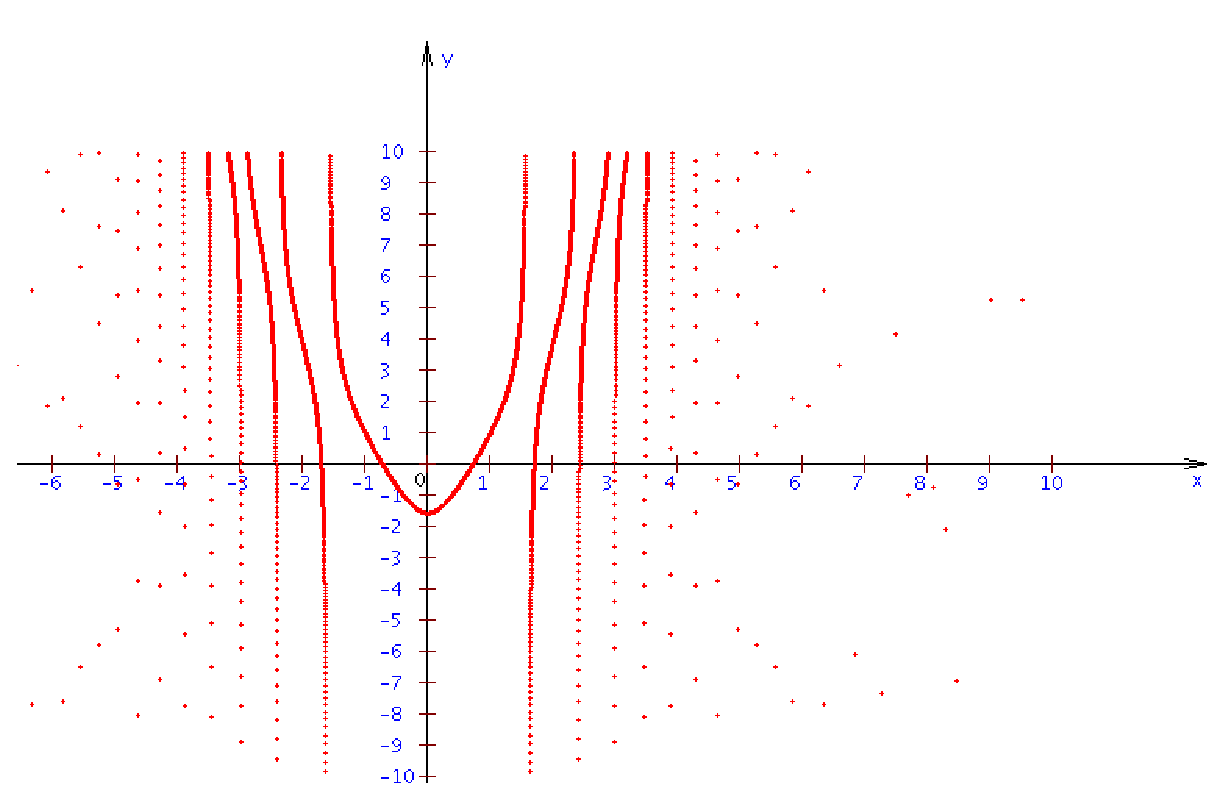
\includegraphics[scale=0.45]{pictures/3_1}
  \caption{ $f=x^2+\mathbf{tg}(x^2-1)$}
  \label{301}
\end{figure}

\eject
To get the graphs of several functions in one figure you must enclose the list 
of these functions in square brackets, as in the following example.

\underline{Example 2. }

%enddelete

\begin{verbatim}
SPACE = R64[x, y, z];
\set2D(-10, 10, -10, 10);
f = \sin(x); 
p = \plot([f, \tg(x)]);
\end{verbatim}
%begindelete

 \ex{$f=sin(x);$}{fig. \ref{3_3}. }

\begin{figure}[!h]
  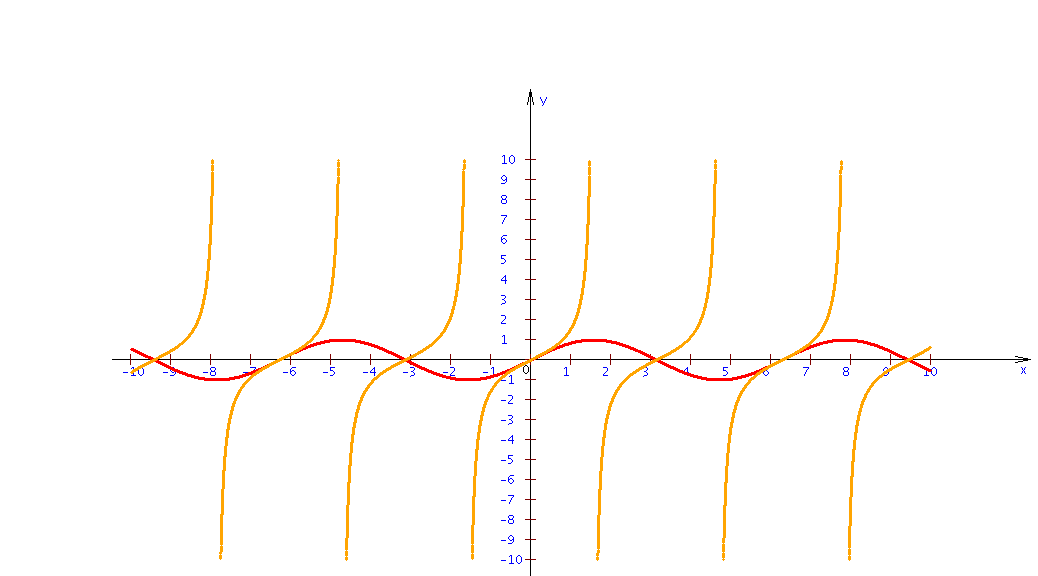
\includegraphics[width=274.6pt,height=152.38pt]{pictures/3_3}
  \caption{ $f = \sin(x)$ and $g = \mathbf{tg}(x)$}
  \label{3_3}
\end{figure}

\underline{Example 3. }

%enddelete

\begin{verbatim}
SPACE = R64[x, y, z];
\set2D(-10, 10, 0, 2);
f = \unitBox(x,3); 
p = \plot(f);
\end{verbatim}
%begindelete

%\ex{$f=unitBox(x,3);$}{fig. \ref{3_3}. }

%\begin{figure}[!h]
%  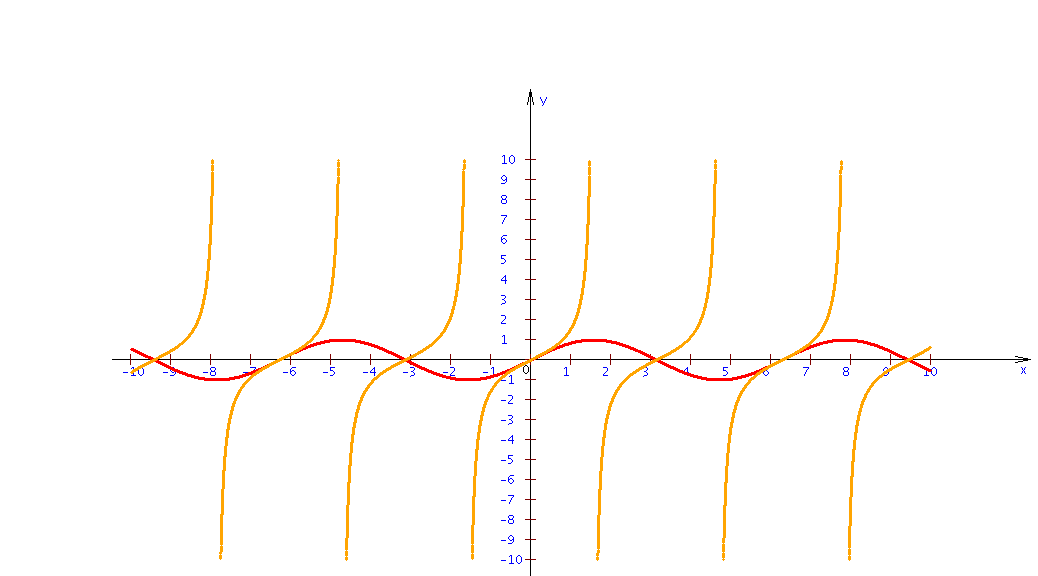
\includegraphics[width=274.6pt,height=152.38pt]{pictures/3_3}
%  \caption{ $f = \sin(x)$ и $g = \tg(x)$}
%  \label{3_3}
%\end{figure}


\underline{Example 4. }

%enddelete

\begin{verbatim}
SPACE = R64[x, a, b, c];
\set2D(0, 2\pi, 0, 2);
\plot(a\sin(bx) + c);
\end{verbatim}

%begindelete

%  \ex{$f=sin(x);$}{pict. \ref{3_3}. }
% 
% \begin{figure}[!h]
%   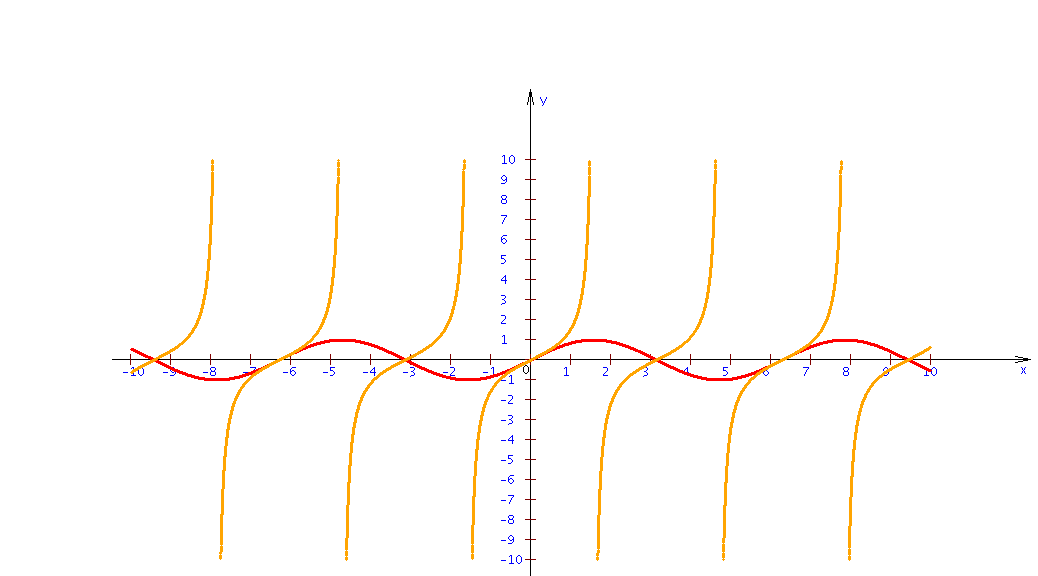
\includegraphics[width=274.6pt,height=152.38pt]{pictures/3_3}
%   \caption{Графики функций $f = \sin(x)$ и $g = \tg(x)$}
%   \label{3_3}
% \end{figure}
%enddelete

%begindelete
\underline{Example 5. }
%enddelete
\vspace*{-2mm}
\begin{verbatim}
SPACE = R64[x, y, z];
\set2D(-10, 10, -10, 10,'a','b','title');
f = x^2; 
p = \plot(f);
\end{verbatim}
\vspace*{-2mm}

%begindelete
\underline{Example 6. }
%enddelete
\vspace*{-2mm}
\begin{verbatim}
SPACE = R64[x, y, z];
\set2D(-10, 10, -10, 10);
f = x; 
p = \plot(f,'dash');
\end{verbatim}
\vspace*{-2mm}

%begindelete
\underline{Example 7. }
%enddelete
\vspace*{-2mm}
\begin{verbatim}
SPACE = R64[x, y, z]; 
f = x; 
p = \plot(f,[-5,5],'arrow');
\end{verbatim}
\vspace*{-2mm}

%begindelete
\underline{Example 8. }
%enddelete
\vspace*{-2mm}
\begin{verbatim}
SPACE = R64[x, y, z]; 
\set2D(-10, 10, -10, 10);
\plot([x,-x],'arrow');
\end{verbatim}
\vspace*{-2mm}
 
\subsection{Plots of parametric functions}  
To obtain the plot of parametric function \{$f=x(t)$, $g=y(t)$\} the command 
\comm{paramPlot}{([f, g], [t0, t1])} is used, where $[t0, t1]$ is an interval of variation of $t$.
Another version of the command:  \comm{paramPlot}{([f, g], [t0, t1], 'options')}, where $[t0, t1]$~--- the range of values for the parameter change, 
'options'~---  the following values:\\
1)'dash'~--- schedule will be a dashed line;\\ 
2)'arrow'~---  the last point on the graph is drawn with an arrow;\\
3)'dashAndArrow'~--- schedule will be a dashed line and the last point of the graph is drawn with an arrow.\\

%begindelete

\underline{Example 1. }


\nopagebreak
%enddelete
\vspace*{-2mm}
\begin{verbatim}
SPACE = R64[x, y, z];
g = \sin(x); 
k = \cos(x); 
f = \paramPlot([g, k], [0, 2\pi]);
\end{verbatim}
\vspace*{-2mm}

%begindelete
\ex{$g=sin(x); k=cos(x);$}{fig. \ref{3_4}.}
\begin{figure}[h!]
 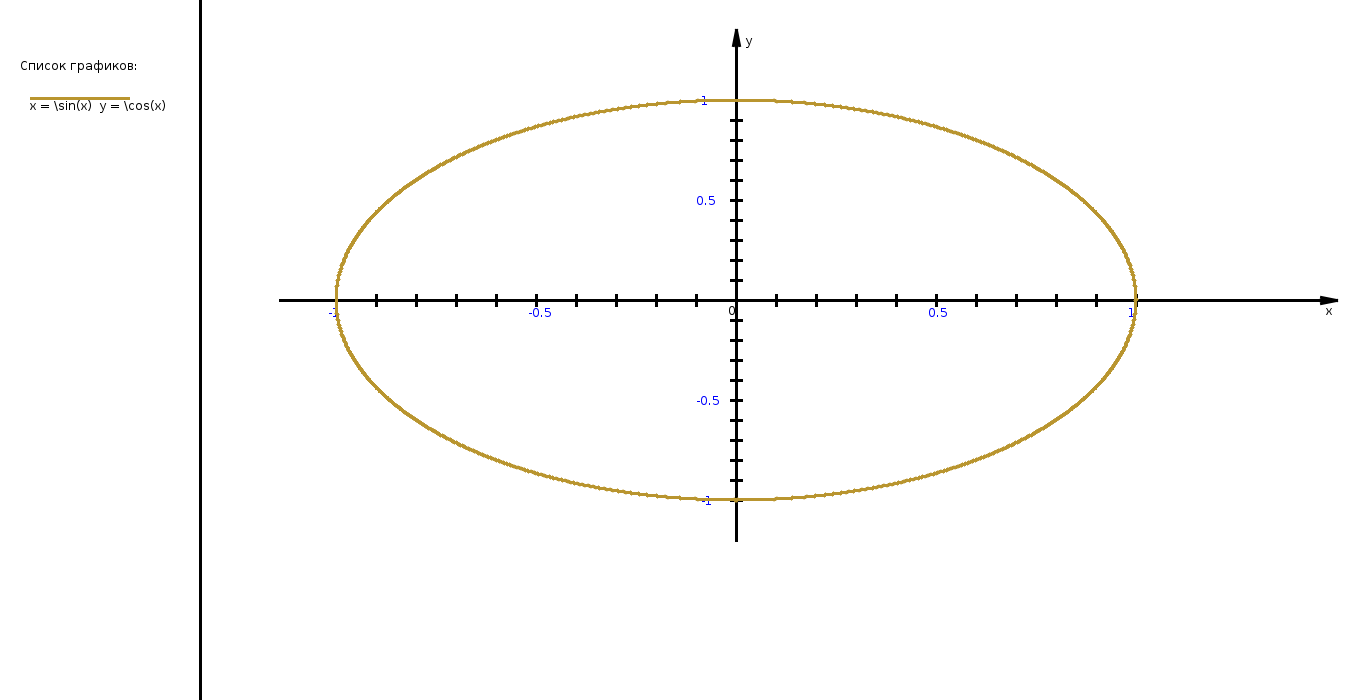
\includegraphics[scale=0.26]{pictures/2_1}
\vspace*{-10mm}
\caption{}
\label{3_4}
\end{figure}
%enddelete


%begindelete
\eject
\underline{Example 2. }


%enddelete
\vspace*{-2mm}
\begin{verbatim}
SPACE = R64[x, y, z];
g = x\sin(x);
k = x\cos(x);
f = \paramPlot([g, k], [0, 5\pi]);
\end{verbatim}
\vspace*{-2mm}

%begindelete
\ex{$g=x\sin(x); k=x\cos(x);$}{fig. \ref{2_2}.}
\begin{figure}[h!]
 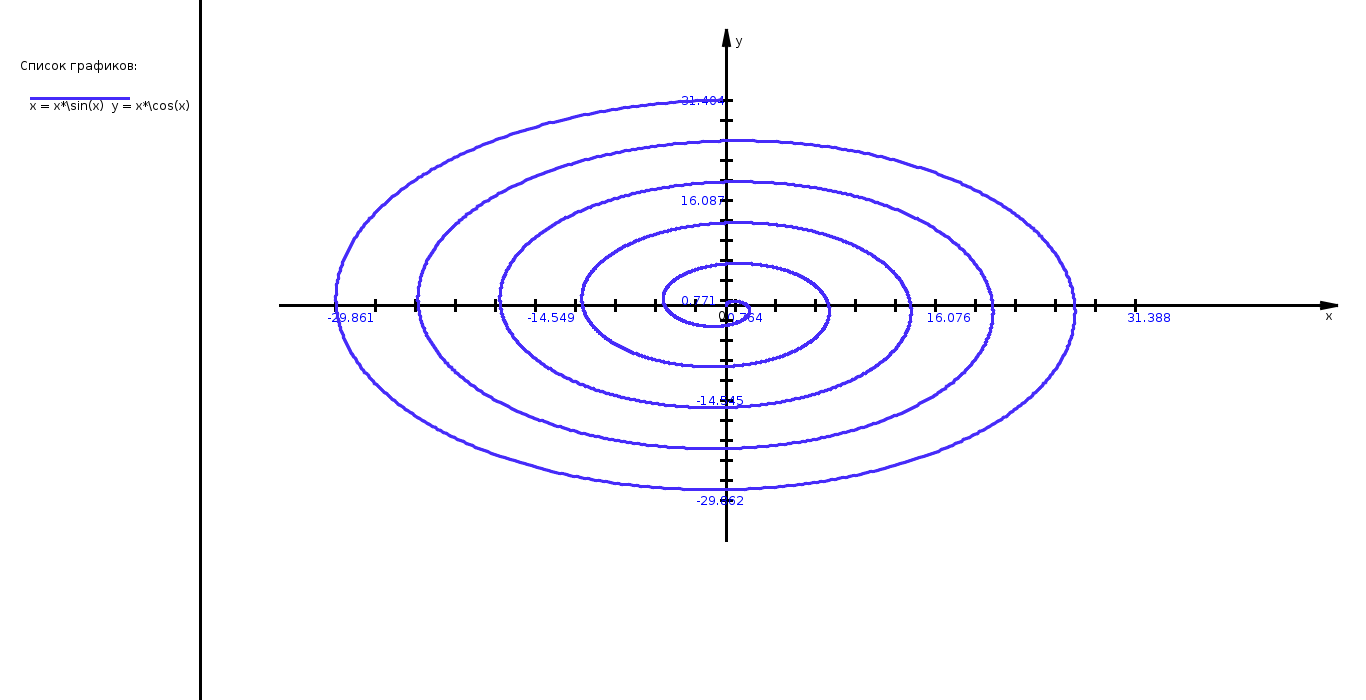
\includegraphics[scale=0.3]{pictures/2_2}
\vspace*{-10mm}
\caption{}
\label{2_2}
\end{figure}



\underline{Example 3. }

%enddelete

\vspace*{-2mm}
\begin{verbatim}
SPACE = R64[x, y, z];
g = 2\cos(x)+\cos(2x); 
k = 2\sin(x)-\sin(2x);
f = \paramPlot([g, k], [0, 2\pi]);
\end{verbatim}
\vspace*{-2mm}

%begindelete
\ex{$g=2\cos(x)+\cos(2x); k= 2\sin(x)-\sin(2x);$}{fig. \ref{2_3}.}
\begin{figure}[h!]
 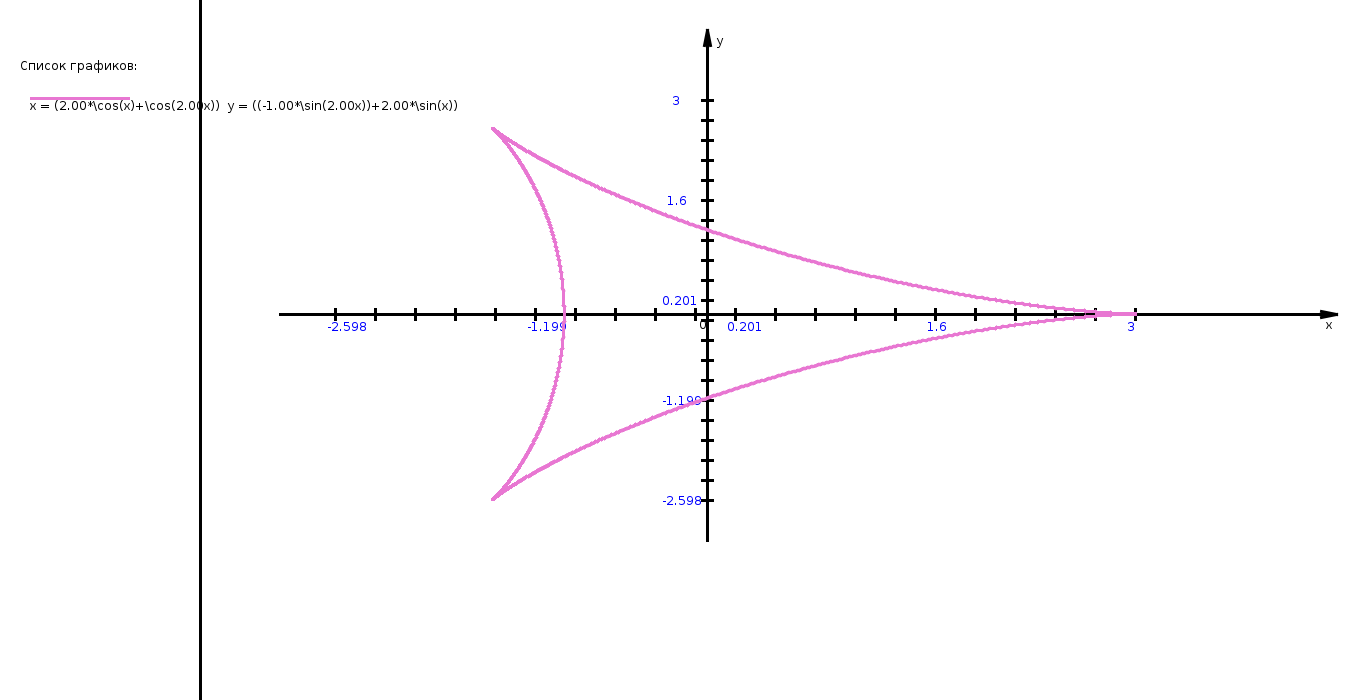
\includegraphics[scale=0.3]{pictures/2_3}
\vspace*{-10mm}
\caption{}
\label{2_3}
\end{figure}

\eject
\underline{Example 4. }


%enddelete

\vspace*{-2mm}
\begin{verbatim}
SPACE = R64[x, y, z];
g = 2\sin(x)^3; 
k = 2\cos(x)^3;
f = \paramPlot([g, k], [0, 2\pi]);
\end{verbatim}
\vspace*{-2mm}


%begindelete
\ex{$g=2\sin(x)^3; k= 2\cos^3(x)$}{fig. \ref{2_4}.}
\begin{figure}[h!]
 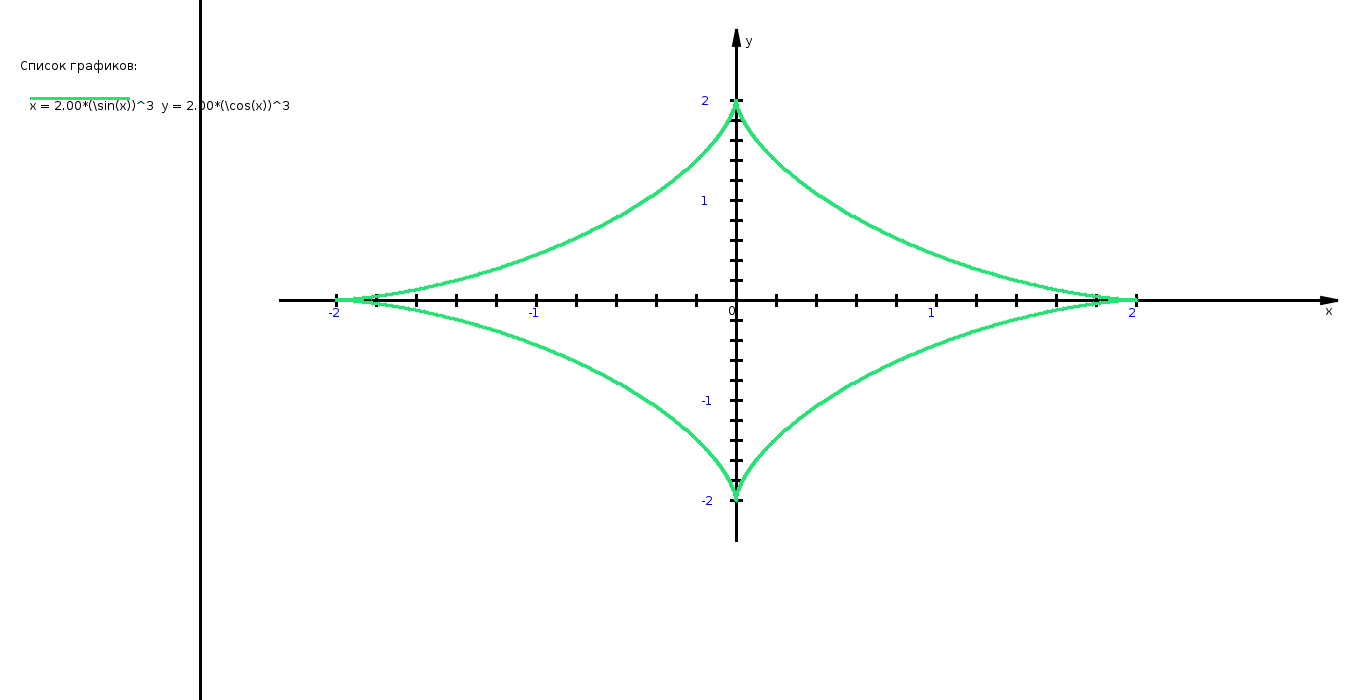
\includegraphics[scale=0.3]{pictures/2_4}
\vspace*{-10mm}
\caption{}
\label{2_4}
\end{figure}



\underline{Example 5. }
%enddelete

\vspace*{-2mm}
\begin{verbatim}
SPACE = R64[x, y, z];
g = (1+\cos(x))\cos(x); 
k = (1+\cos(x))\sin(x);
f = \paramPlot([g, k], [0, 2\pi]);
\end{verbatim}
\vspace*{-2mm}

%begindelete
\ex{$g=(1+\cos(x))\cos(x);k= (1+\cos(x))\sin(x);$}{fig. \ref{2_5}.}
\begin{figure}[h!]
 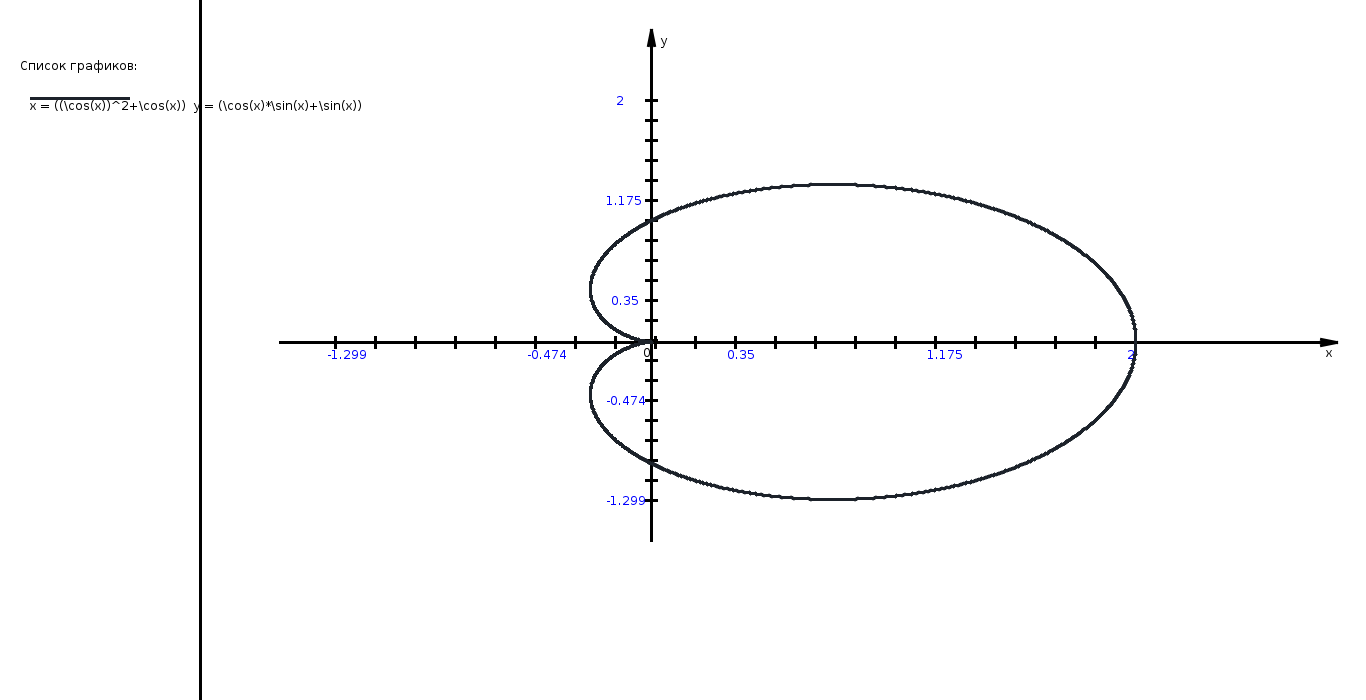
\includegraphics[scale=0.3]{pictures/2_5}
\vspace*{-10mm}
\caption{}
\label{2_5}
\end{figure}

%begindelete
\eject
\underline{Example 6. }
%enddelete


\vspace*{-2mm}
\begin{verbatim}
SPACE = R64[x, y, z];
g = \sin(x)(\exp(\cos(x))-2\cos(4x)+\sin(x/12)^5);
k = \cos(x)(\exp(\cos(x))-2\cos(4x)+\sin(x/12)^5);
f = \paramPlot([g, k], [0, 12\pi]);
\end{verbatim}
\vspace*{-2mm}


%begindelete
\ex{$g=\sin(x)(\exp(\cos(x))-2\cos(4x)+\sin^5(x/12));$\\
\hspace*{4mm} $k= \cos(x)(\exp(\cos(x))-2\cos(4x)+\sin^5(x/12));$}{fig. \ref{2_6}.}
\begin{figure}[h!]
 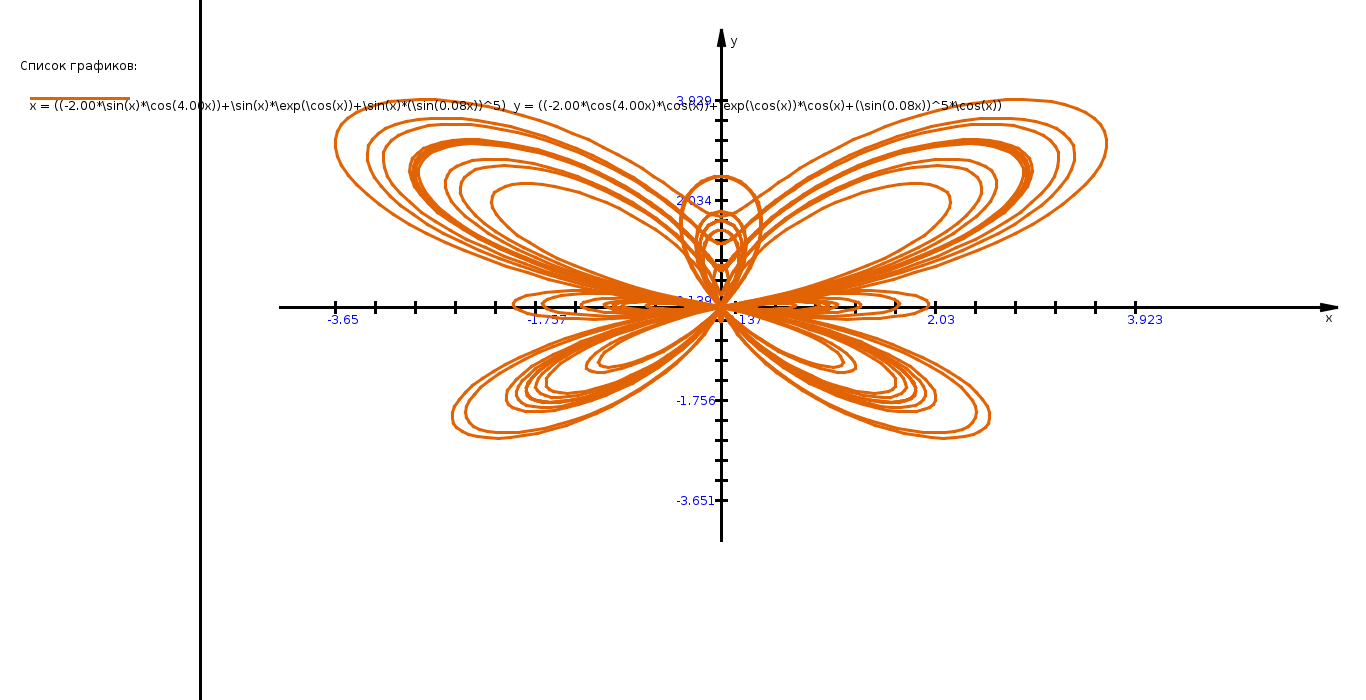
\includegraphics[scale=0.3]{pictures/2_6}
\vspace*{-10mm}
\caption{}
\label{2_6}
\end{figure}


\eject
\underline{Example 7. }
%enddelete


\vspace*{-2mm}
\begin{verbatim}
SPACE = R64[x, y, z];
\set2D('','','','','x(t)','y(t)','paramPlot');
g = \sin(x)(\exp(\cos(x))-2\cos(4x)+\sin(x/12)^5);
k = \cos(x)(\exp(\cos(x))-2\cos(4x)+\sin(x/12)^5);
f = \paramPlot([g, k], [0, 12\pi]);
\end{verbatim}
\vspace*{-2mm}

%begindelete
\eject
\underline{Example 8. }
%enddelete

\vspace*{-2mm}
\begin{verbatim}
SPACE = R64[x, y, z];
g = \sin(x); 
k = \cos(x); 
f = \paramPlot([g, k], [0, 2\pi],'dashAndArrow');
\end{verbatim}
\vspace*{-2mm}

\subsection{Plot of table function} 
To plot a function, which is defined by the table of points you have to execute the command: 
\comm{tablePlot}{([[x_{1},\ldots, x_{n}],[y_{11},\ldots,a_{1n}],\ldots,[y_{k1},\ldots,a_{kn}]])}.\\
Another version of the command:
\comm{tablePlot}{([[x_{1},\ldots, x_{n}],[y_{11},\ldots,a_{1n}],\ldots,[y_{k1},\ldots,a_{kn}]], 'options')}
,where 'options'~--- the following values:\\
1)'dash'~--- schedule will be a dashed line;\\ 
2)'arrow'~---  the last point on the graph is drawn with an arrow;\\
3)'dashAndArrow'~--- schedule will be a dashed line and the last point of the graph is drawn with an arrow.

%begindelete
\underline{Example 1.}
 
 \vspace*{-2mm}
%enddelete

 \begin{verbatim}
SPACE = R64[x, y, z];
 \tablePlot(
   [
     [0, 1, 2, 3, 4, 5],
     [0, 1, 4, 9, 16, 25],
     [0, -1, -2, -3, -4, -5],
     [0, 4, 8, 12, 16, 20]
   ]);
 \end{verbatim}

 %begindelete
\ex{}{fig. \ref{2_7}.}
\begin{figure}[!h]
 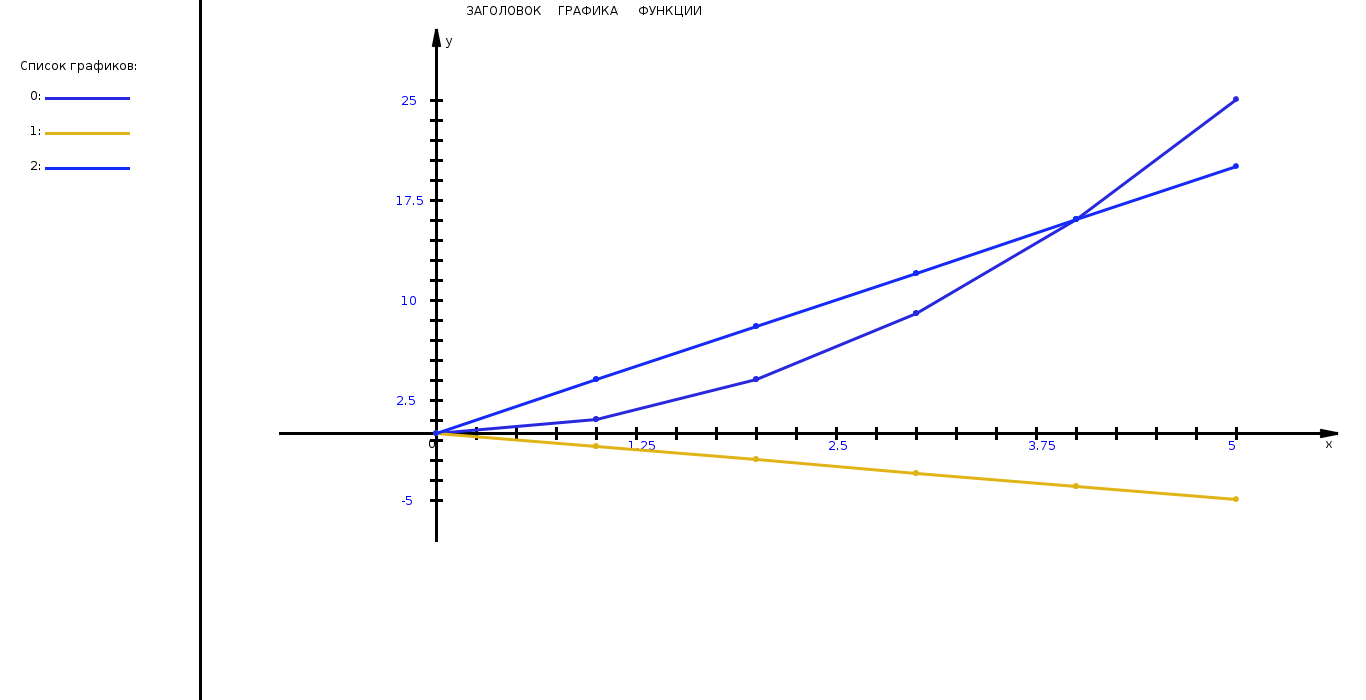
\includegraphics[scale=0.25]{pictures/2_7}
\vspace*{-10mm}
\caption{}
\label{2_7}
\end{figure}


\underline{Example 2.}
 %enddelete

 \vspace*{-2mm}
 \begin{verbatim}
 SPACE=R64[x]; 
\set2D(-1,5,-10,10);
"We have a table function"
A = [[0, 1, 2, 3, 4, 5], [3, 0, 4, 10, 5, 10]];
t = \table (A);
"We approximate this function by a polynomial of degree 4:" 
p = \approximation(t, 4);
"Building the graph of the polynomial:" P = \plot (p, [1,5]);
"Plot a table function:" T = \tablePlot (t);
"We construct both graphs in one coordinate system:" 
\showPlots ([P, T]);
 \end{verbatim}

%begindelete
\ex{}{$0.54x^4-5.64x^3+18.38x^2-17.28x+3.17$\\
\hspace*{4mm} fig. \ref{2_8}.}
\begin{figure}[!h]
 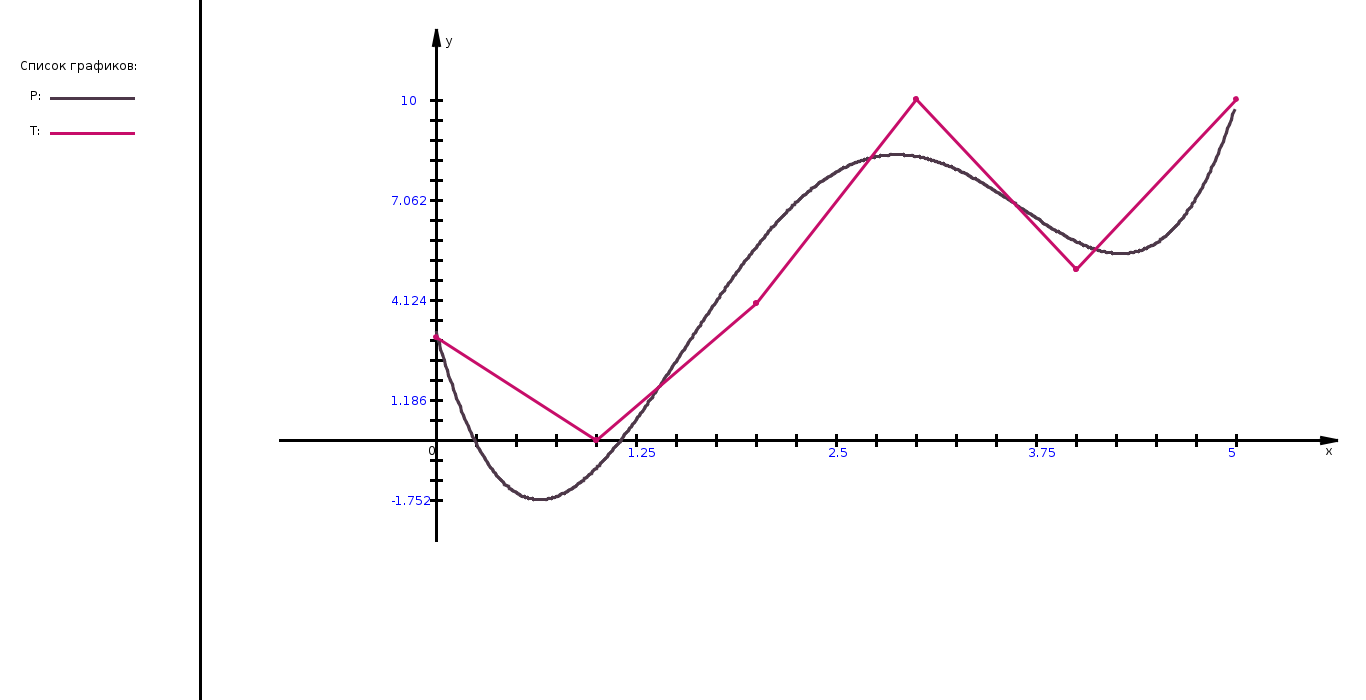
\includegraphics[scale=0.25]{pictures/2_8}
\vspace*{-10mm}
\caption{}
\label{2_8}
\end{figure}
%enddelete

%begindelete
\underline{Example 3.}
 
 \vspace*{-2mm}
%enddelete

 \begin{verbatim}
SPACE = R64[x, y, z];
\set2D(-10, 10, -10, 10, '','', 'Header of Graphics');
 \tablePlot(
   [[-3, -6, -6, -3, 3, 6, 6, 3, -3],
    [6, 3, -3, -6, -6, -3, 3, 6, 6]]);
 \end{verbatim}

%begindelete
\underline{Example 4.}
 
 \vspace*{-2mm}
%enddelete

 \begin{verbatim}
SPACE = R64[x, y, z];
 \tablePlot(
   [[-3, -6, -6, -3, 3, 6, 6, 3, -3],
    [6, 3, -3, -6, -6, -3, 3, 6, 6]],'arrow');
 \end{verbatim}

%begindelete
\underline{Example 5.}
 
 \vspace*{-2mm}
%enddelete

 \begin{verbatim}
SPACE = R64[x, y, z];
 \tablePlot(
   [[-3, -6, -6, -3, 3, 6, 6, 3, -3],
    [6, 3, -3, -6, -6, -3, 3, 6, 6]], 'dash');
 \end{verbatim}

%begindelete
\underline{Example 6.}
 
 \vspace*{-2mm}
%enddelete

 \begin{verbatim}
SPACE = R64[x, y, z];
 \tablePlot(
   [[-3, -6, -6, -3, 3, 6, 6, 3, -3],
    [6, 3, -3, -6, -6, -3, 3, 6, 6]], 'dashAndArrow');
 \end{verbatim}

\subsection{Functions that are defined on the points table of values}
Plotting functions on the points given by the tabulated values use the command: 
\comm{pointsPlot}{([[x_{1},\ldots, x_{n}],[y_{1},\ldots,y_{n}]], [s_{1},\ldots,s_{n}], [kv_{1},\ldots,kv_{n}], [kg_{1},\ldots,kg_{n}])},\\
where $s_{n}$~--- signature points, $kv_{n}$~--- rate of rotation about the point (ranges from 0 to 7, and signifies a shift in the ($kv_{n}$ * 45) degrees), 
$kg_{n}$~--- shift factor along the axis $OX$ (if it is negative then the displacement is to the left).
The reduced variants of this command:
\comm{pointsPlot}{([[x_{1},\ldots, x_{n}],[y_{1},\ldots,y_{n}]], [s_{1},\ldots,s_{n}])}
or
\comm{pointsPlot}{([[x_{1},\ldots, x_{n}],[y_{1},\ldots,y_{n}]], [s_{1},\ldots,s_{n}], [kv_{1},\ldots,kv_{n}])}
or
\comm{pointsPlot}{([[x_{1},\ldots, x_{n}],[y_{1},\ldots,y_{n}]], [s_{1},\ldots,s_{n}], [kv_{1},\ldots,kv_{n}], [kg_{1},\ldots,kg_{n}])}
 
%begindelete
\underline{Example 1.}
 
 \vspace*{-2mm}
%enddelete

\begin{verbatim}
\set2D(-10, 10, -10, 10);
\pointsPlot(
   [[0, 1, 2],
     [0, 1, 4]],['a','b','c']);
\end{verbatim}

%begindelete
\underline{Example 2.}
 
 \vspace*{-2mm}
%enddelete

\begin{verbatim}
\pointsPlot(
   [[0, 1, 2],
     [0, 1, 4]],['a','b','c'],[0,2,4]);
\end{verbatim}

%begindelete
\underline{Example 3.}
 
 \vspace*{-2mm}
%enddelete

\begin{verbatim}
\pointsPlot(
   [[0, 1, 2],
     [0, 1, 4]],['a','b','c'],[0,2,4],[0,-5,5]);
\end{verbatim}

%begindelete
\underline{Example 4.}
 
 \vspace*{-2mm}
%enddelete

\begin{verbatim}
\pointsPlot(
   [[0, 1, 2],
     [0, 1, 4]]);
\end{verbatim}

%begindelete
\underline{Example 5.}
 
 \vspace*{-2mm}
%enddelete

\begin{verbatim}
SPACE = R64[x, y, z];
f1=\tablePlot([[1, 1], [1, 5]]);
f2=\tablePlot([[1, 5], [1, 1]]);
f3=\tablePlot([[5, 5], [1, 5]]);
f4=\tablePlot([[1, 5], [5, 5]]);
f5=\pointsPlot([[1, 1, 5, 5],[1, 5, 5, 1]],['A','B','C','D'],[6,0,0,2]);
\showPlots([f1, f2, f3, f4, f5]);
\end{verbatim}

%begindelete
\underline{Example 6.}
 
 \vspace*{-2mm}
%enddelete

\begin{verbatim}
SPACE = R64[x, y, z];
f1=\tablePlot([[1, 1], [1, 5]]);
f2=\tablePlot([[1, 5], [1, 1]]);
f3=\tablePlot([[5, 5], [1, 5]]);
f4=\tablePlot([[1, 5], [5, 5]]);
f5=\pointsPlot([[1, 1, 5, 5],[1, 5, 5, 1]],['A','B','C','D'],[6,0,0,2]);
\showPlots([f1, f2, f3, f4, f5], 'noAxes');
\end{verbatim}

\subsection{Construction of various plots of functions in one coordinate system}
To construct the plots of functions defined in different ways, you must first build a plot of each function and then execute the command  
\comm{showPlots}{([f_1, f_2, \ldots, f_n])}.

Another version of the command:
\comm{showPlots}{([f1, f2, f3, f4], 'noAxes')}, where 'noAxes'~--- parameter indicating image graphics without axes.
or
\comm{showPlots}{([f1, f2, f3, f4], 'lattice')}, where 'lattice'~--- parameter indicating the image graph with the lattice.

%begindelete
\underline{Example 1.}
 
 \vspace*{-2mm}
%enddelete

\begin{verbatim}
SPACE = R64[x, y, z];
\set2D(-20, 20, -20, 20);
f1 = \plot(\tg(x));
f2 = \tablePlot([[0, 1, 4, 9, 16, 25], [0, 1, 2, 3, 4, 5]]);
f3 = \paramPlot([\sin(x), \cos(x)], [-10, 10]);
f4=\tablePlot([[0, 1, 4, 9, 16, 25], [0, -1, -2, -3, -4, -5]]);
\showPlots([f1, f2, f3, f4]);
\end{verbatim}
%begindelete
\ex{}{fig. \ref{3_6}.}
\begin{figure}[!ht]
 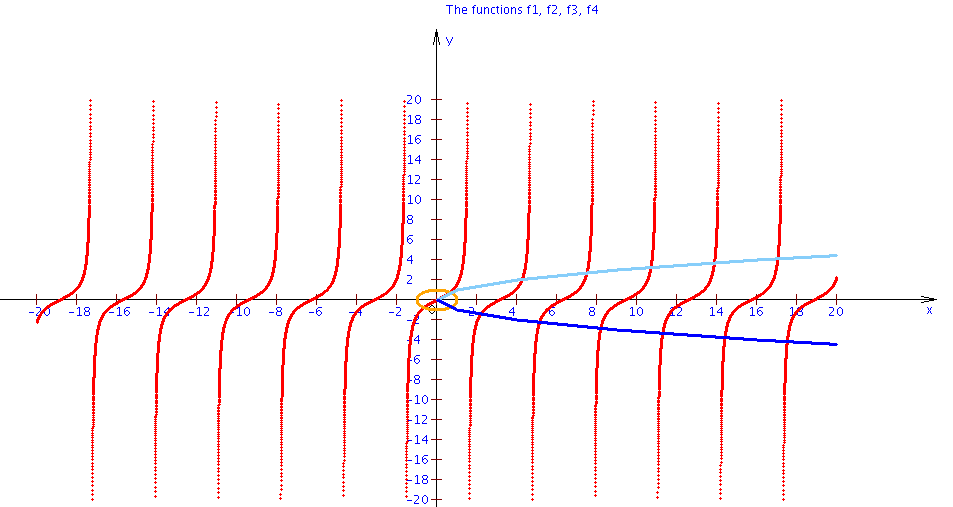
\includegraphics[scale=0.6]{pictures/3_6}
\caption{Graphs of functions defined in different ways}
\label{3_6}
\end{figure}
%enddelete

%begindelete
\underline{Example 2.}
 
 \vspace*{-2mm}
%enddelete

 \begin{verbatim}
p1=\tablePlot([[-1, -3, 3, 3, -3, -3],[4, 3, 3, -3 , -3, 3]]);
p2=\tablePlot([[5, 5, 3, 3, 5, -1],[4, -2, -3, 3, 4, 4]]);
p3=\tablePlot([[-3, -1, -1],[-3, -2, 4]], 'dash');
p4=\tablePlot([[-1, 5],[-2, -2]], 'dash');
\showPlots([p1,p2,p3,p4], 'noAxes');
 \end{verbatim}

%begindelete
\underline{Example 3.}
 
 \vspace*{-2mm}
%enddelete

 \begin{verbatim}
p1=\tablePlot([[-1, -3, 3, 3, -3, -3],[4, 3, 3, -3, -3, 3]]);
p1p=\pointsPlot([[-1, -3, 3, 3, -3],[4, 3, 3, -3 , -3]],['F','B','C','D','A'],[0,0,0,4,4]);
p2=\tablePlot([[5, 5, 3, 3, 5, -1],[4, -2, -3, 3, 4, 4]]);
p3=\tablePlot([[-3, -1, -1],[-3, -2, 4]],'dash');
p4=\tablePlot([[-1, 5],[-2, -2]],'dash');
p2p=\pointsPlot([[5, 5, -1 ],[4, -2, -2]],['G','H','E'],[0,4,4]);
\showPlots([p1,p2,p3,p4,p1p,p2p], 'noAxes');
 \end{verbatim}

\subsection{Construction of graphs}
To construct the graph, use the command
\comm{plotGraph}{([[a_{11},\ldots,a_{1n}],\ldots,[a_{n1},\ldots,a_{nn}]], [[x_{1},\ldots, x_{n}],[y_{1},\ldots,y_{n}]])}, 
where $[[a_{11},\ldots,a_{1n}],\ldots,[a_{n1},\ldots,a_{nn}]]$ ~--- adjacency matrix, $[[x_{1},\ldots, x_{n}],[y_{1},\ldots,y_{n}]]$ ~--- matrix of coordinates.

%begindelete
\underline{Example 1. }
%enddelete

\vspace*{-2mm}
\begin{verbatim}
SPACE = R64[x, y, z];
\plotGraph([[0,1,1,0,1,0],[1,0,0,1,1,0],[1,0,0,0,1,1],[0,1,0,0,0,0],
[1,1,1,0,0,1],[0,0,1,0,1,0]],[[3,2,4,1,3,5],[3,2,2,1,1,1]]);
\end{verbatim}
%begindelete
\ex{}{pict. \ref{4_1}.}
\begin{figure}[!ht]
 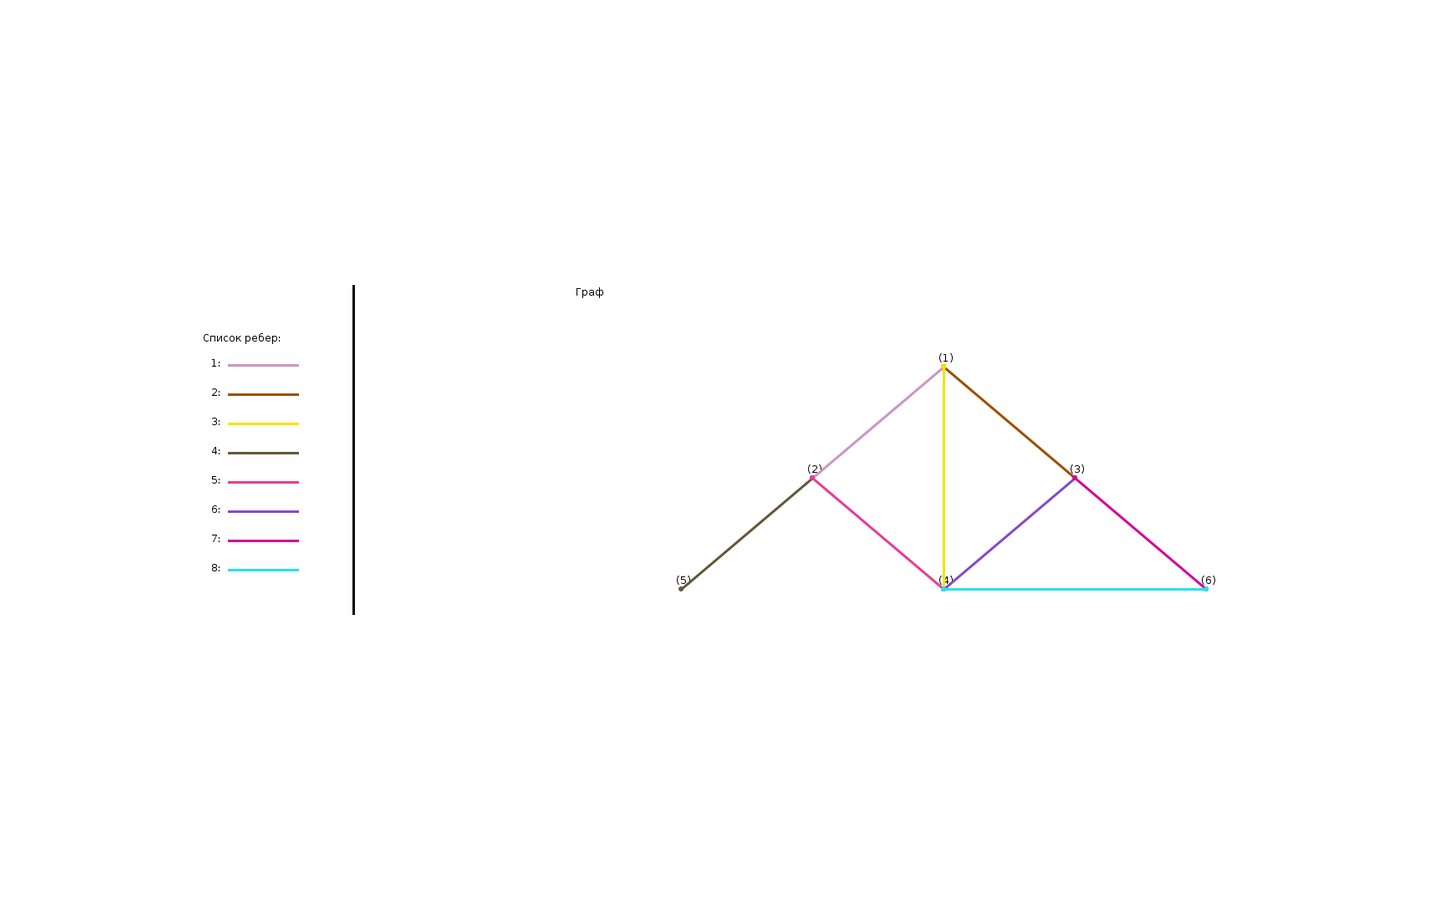
\includegraphics[scale=0.4]{pictures/4_1}
\caption{graph}
\label{4_1}
\end{figure}
%enddelete

In addition, you can run only with the first parameter
\comm{plotGraph}{([[a_{11},\ldots,a_{1n}],\ldots,[a_{n1},\ldots,a_{nn}]])}, 
where $[[a_{11},\ldots,a_{1n}],\ldots,[a_{n1},\ldots,a_{nn}]]$ ~--- adjacency matrix.

%begindelete
\underline{Example 2. }
%enddelete

\vspace*{-2mm}
\begin{verbatim}
SPACE = R64[x, y, z];
\plotGraph([[0,1,1,0,1,0],[1,0,0,1,1,0],[1,0,0,0,1,1],[0,1,0,0,0,0],
[1,1,1,0,0,1],[0,0,1,0,1,0]]);
\end{verbatim}
%begindelete
\ex{}{pict. \ref{4_2}.}
\begin{figure}[!ht]
 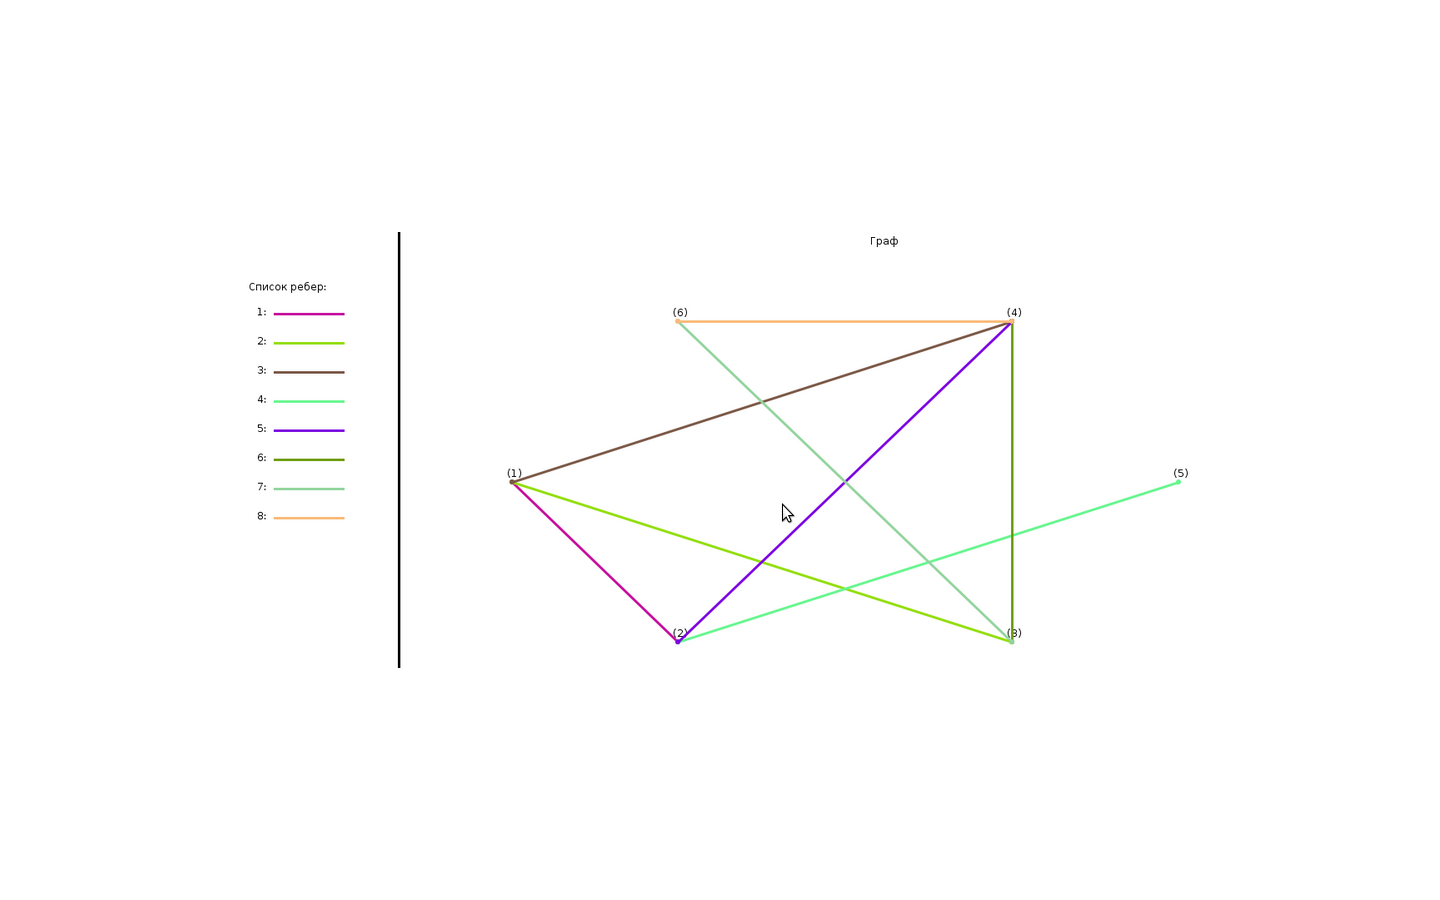
\includegraphics[scale=0.4]{pictures/4_2}
\caption{graph}
\label{4_2}
\end{figure}
%enddelete

You need to run a single numeric parameter
\comm{plotGraph}{(N)}, 
where $N$ ~--- the number of vertices in a graph.

%begindelete
\underline{Example 3. }
%enddelete

\vspace*{-2mm}
\begin{verbatim}
SPACE = R64[x, y, z];
\plotGraph(6);
\end{verbatim}
%begindelete
\ex{}{pict. \ref{4_3}.}
\begin{figure}[!ht]
 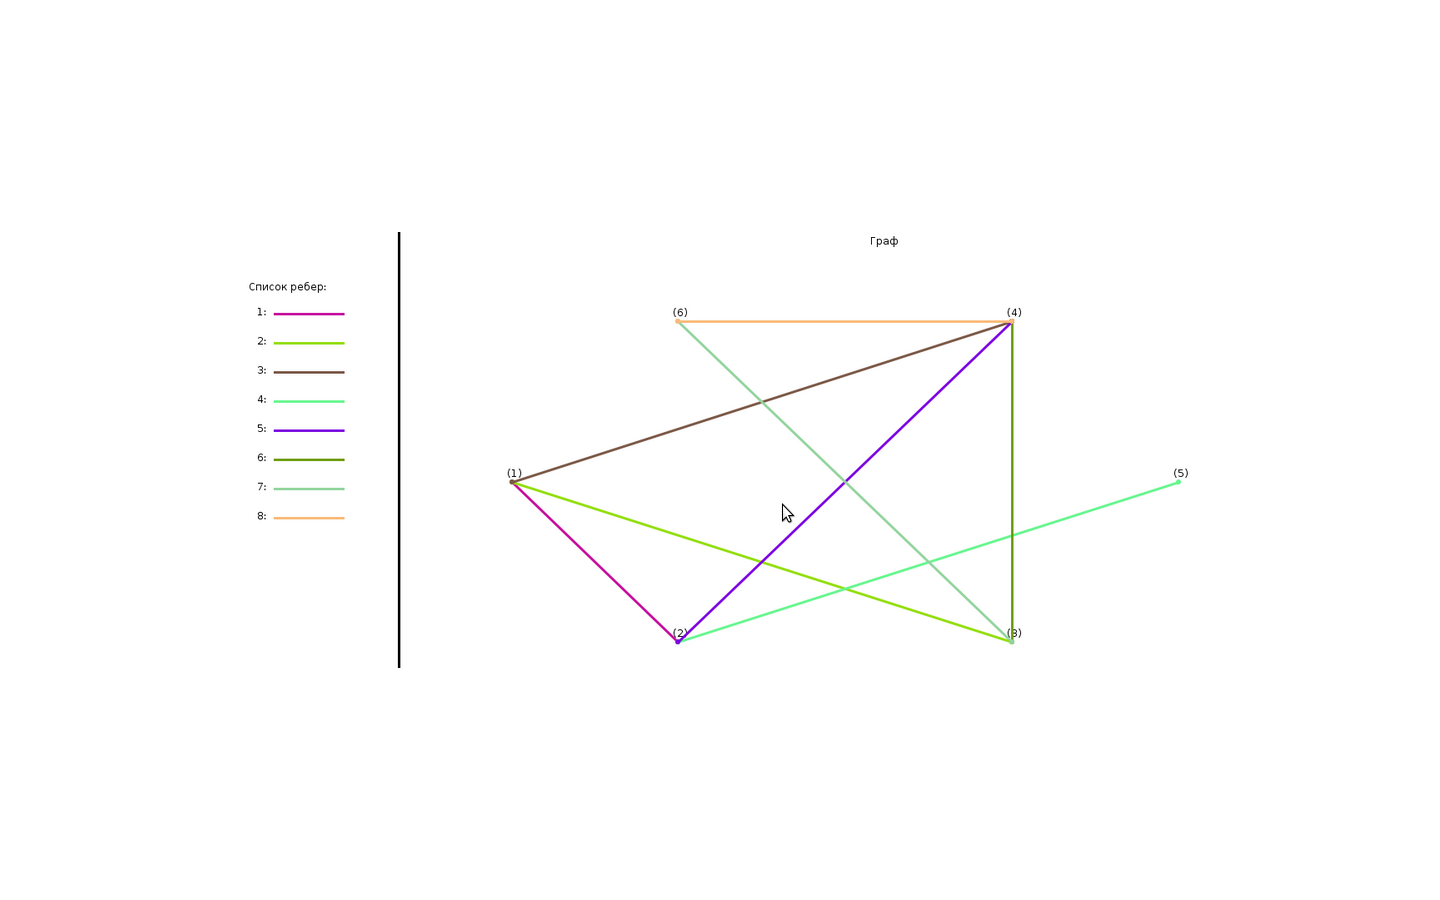
\includegraphics[scale=0.4]{pictures/4_2}
\caption{graph}
\label{4_3}
\end{figure}
%enddelete

\section{Plots 3D of explicit functions} 
You can build 3D graphs of the functions that are defined explicitly. 
 
To obtain the plot 3D of an explicit function $f=f(x,y)$ the command 
\comm{plot3d}{(f, [x0, x1, y0, y1])}, 
 is used, where $[x0, x1]$ is an interval on the axis $OX$, $[y0, y1]$ is an interval on the axis $OY$.

The obtained plot can be rotated and to increase or decrease.

Moving the mouse holding down the left <<mouse>> button causes the rotation of the coordinate system of schedule.
After stopping the movement of the <<mouse>> graphics are redrawn in the new rotated coordinate system.
 
Moving the mouse holding down the left mouse button while pressing ${\it Shift}$ button leads 
to a change in image scale. After stopping the movement of the <<mouse>> graphics are redrawn in the new scale.

%begindelete
\underline{Example. }

\vspace*{-2mm}
%enddelete

\begin{verbatim}
SPACE = R64[x, y, z];
f = x^2 / 20 + y^2 / 20;
\plot3d(f, [-20, 20, -20, 20]);
\end{verbatim}

\begin{verbatim}
SPACE = R64[x, y, z];
\plot3d([x / 20 + y^2 / 20, x^2 / 20 + y / 20], [-20, 20, -20, 20]);
\end{verbatim}

\begin{verbatim}
SPACE = R64[x, y, a, b];
f = ax^2 / 20 + by^2 / 20;
\plot3d(f, [-20, 20, -20, 20]);
\end{verbatim}

Sphere 

\begin{verbatim}
SPACE=R64[u,v];
\paramPlot3d([[\cos(u)\cos(v)],[\sin(u)\cos(v)],[\sin(v)]], [-\pi, \pi, -\pi/2, \pi/2]);
\end{verbatim}

Thor 

\begin{verbatim}
SPACE=R64[u,v];
\paramPlot3d([[\cos(u)(\cos(v)+3)],[\sin(u)(\cos(v)+3)],[\sin(v)]], [-\pi, \pi, -\pi, \pi]);
\end{verbatim}

Spiral

\begin{verbatim}
SPACE=R64[u,v];
\paramPlot3d([[\cos(u)(\cos(v)+3)],[\sin(u)(\cos(v)+3)],[\sin(v)+u]], [-2\pi, 2\pi, -\pi, \pi]);
\end{verbatim}

Logarithmic spiral 

\begin{verbatim}
SPACE=R64[u,v];
\paramPlot3d([[u\cos(u)(\cos(v)+1)],[u\sin(u)(\cos(v)+1)],[u\sin(v)]], [0, 3\pi, -\pi, \pi]);
\end{verbatim}

"Seashell" 

\begin{verbatim}
SPACE=R64[u,v];
\paramPlot3d([[u\cos(u)(\cos(v)+1)],[u\sin(u)(\cos(v)+1)],[u\sin(v)-(((u+3)/8)\pi)^2-20]], [0, 8\pi, -\pi, \pi]);
\end{verbatim}

Shamrock 

\begin{verbatim}
SPACE=R64[u,v];
\paramPlot3d([[\cos(u)\cos(v)+3\cos(u)(1.5+\sin(1.5u/2))],[\sin(u)\cos(v)+3\sin(u)(1.5+\sin(1.5u/2))],[\sin(v)+2\cos(1.5u)]], [-2\pi, 2\pi, -\pi, \pi]);
\end{verbatim}

Dini surface 

\begin{verbatim}
SPACE=R64[u,v];
\paramPlot3d([[\cos(u)\sin(v)],[\sin(u)\sin(v)],[\cos(v)+\lg(\tg(v/2))+0.2u-4]], [0, 4\pi, 0.0001, 2]);
\end{verbatim}

Tape Mobius

\begin{verbatim}
SPACE=R64[u,v];
\paramPlot3d([[(1+v/2\cos(u/2))\cos(u)],[(1+v/2\cos(u/2))\sin(u)],[v/2\sin(u/2)]], [0, 2\pi, -1, 1]);
\end{verbatim}

Cube

\begin{verbatim}
SPACE=R64[u,v];
\paramPlot3d([[u,v,5,u,v,-5],[v,5,u,v,-5,u],[5,u,v,-5,u,v]], [-5, 5, -5, 5]);
\end{verbatim}

Cylinder

\begin{verbatim}
SPACE=R64[u,v];
\paramPlot3d([[5\cos(u)],[5\sin(u)],[v]], [-5, 5, -5, 5]);
\end{verbatim}

Cone 

\begin{verbatim}
SPACE=R64[u,v];
\paramPlot3d([[\cos(u) * (5 * (1 - v/6))],[\sin(u) * (5 * (1 - v/6))],[v]], [-6, 6, 0, 6]);
\end{verbatim}

Truncated cone 

\begin{verbatim}
SPACE=R64[u,v];
\paramPlot3d([[\cos(u) * (5 * (1 - v/6) + 1 * v/6)],[\sin(u) * (5 * (1 - v/6) + 1 * v/6) ],[v]], [-5, 5, -5, 5]);
\end{verbatim}

Hourglass

\begin{verbatim}
SPACE=R64[u,v];
\paramPlot3d([[\cos(u) * (5 * (0.5 - v/6) + 0.01*v/6)],[\sin(u) * (5 * (0.5 - v/6) + 0.01*v/6)],[v]], [0, 2\pi, 0, 2\pi]);
\end{verbatim}


%begindelete
 
\ex{$f=x^2/20+y^2/20;$\\
\hspace*{4mm} $plot3d(f, [-20, 20, -20, 20]);$\\
\hspace*{4mm} $plot3d([x/20+y^2/20, x^2/20+y/20], [-20, 20, -20, 20]);$}
{fig. \ref{3_7}.}

\begin{figure}[!ht]
  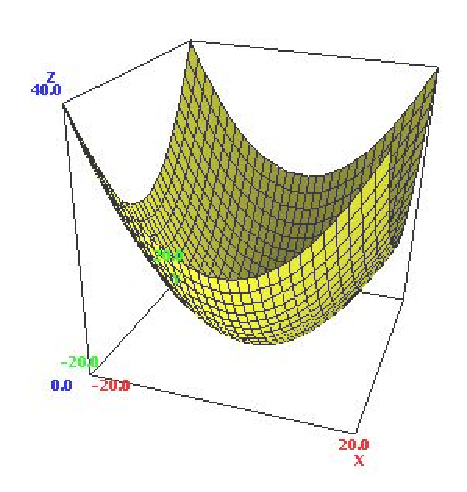
\includegraphics[width=138pt, height=146pt]{pictures/3_7}
  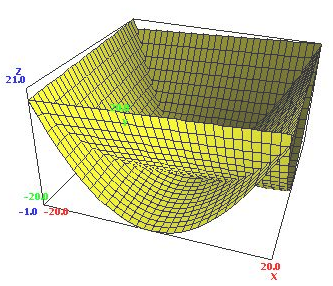
\includegraphics[width=166.5pt, height=143pt]{pictures/3_8}
  \caption{Plots 3D of  functions}
  \label{3_7}
\end{figure}
%enddelete


\section{Ploting of 3D graphs of functions that are defined implicitly} 
You can build 3D graphs of the functions that are defined implicitly. 
 
To construct the graph of an implicit function $ f(x,y,z)=0$ use the command 

 \comm{implicitPlot3d}{(f, x0, x1, y0, y1,z0, z1)}, 

where the numbers $xMin, xMax, yMin, yMax, zMin, zMax$  set the box in the space, 
which is represented by an implicit function. 

You can specify only one function, like this

 \comm{implicitPlot3d}{(f)}

in this case it is assumed that there will be shows the function $ f $ in the cube 
$ 20\times 20 \times 20$,
 which is placed on a center origin.

You can rotate the coordinate system by moving the mouse pointer while holding down the left button.
You can move the coordinate system by moving the mouse pointer while holding down the right button.

It is possible, optionally, to specify the coordinates of the light source, the color of the surface and the grid size. The default grid of 50 points on each edge of the box.

The color format $RGB$ (red, green, blue) is given a number

$R * 256 * 256+ G *256 + B$,

 where each letter denotes a non-negative integer not exceeding 255.
For example, $ 255 * 256 * 256 $ --- red, and $ 255 * 256 * 256 + 255 * $ 256 --- yellow (red + green).

Allowed, in addition, the following sets of arguments:

$(F, xMin, xMax, yMin, yMax, zMin, zMax, gridSize)$,

$(F, xMin, xMax, yMin, yMax, zMin, zMax, lightX, lightY, lightZ, gridSize)$,

$(F, xMin, xMax, yMin, yMax, zMin, zMax, lightX, lightY, lightZ, color, gridSize)$.

%begindelete
\underline{Example. }

\vspace*{-2mm}
%enddelete


\begin{verbatim}
SPACE = R64[x, y, z];
 
f = -x^2+2y^2+3z^2-25;
\implicitPlot3d( f, -10, 10, -10, 10, -10, 10);
\end{verbatim}

 
Hyperboloid



\begin{verbatim}
SPACE = R64[x, y, z ];
\implicitPlot3d( x^2+ y^2+ z^2-25 , -7, 7, -7, 7, -7, 7,10, 10, 10, 255*256*256, 100);
\end{verbatim}

Red sphere.




\begin{verbatim}
SPACE = R64[x, y, z]; 
f =  \sin(xyz/100) ;
\implicitPlot3d( f , -9,9,-9,9,-9,9, 10,10, 4, 255*256*256+255*256, 50);
\end{verbatim}

Yellow surface with a central symmetry.


\begin{verbatim}
SPACE = R64[x, y, z]; 
f = ((x+2)^2+ (y-2)^2 -1)((x-2)^2+ (y+2)^2 -1)((x+2)^2+ (y+2)^2 -1) ((x-2)^2+ (y-2)^2 -1)(x^2+ y^2 -1); 
\implicitPlot3d( f, -10, 10, -10, 10, -10, 10 );
\end{verbatim}

Organ pipes.
  
\chapter{Environment for mathematical objects}
\section{Setting of environment}

The definition of any mathematical object, a number or function, a matrix or symbol, involves the definition of some environment, that is, the space which contains this object. 
To select the environment you have to set the {\it algebraic structure}.  
This algebraic structure is defined by numeric sets, algebraic operations in these sets and variable names.

First of all any user have to set an environment in Mathpar.

By default, a space of the four real variables $\mathbb{R}64[x,y,z,t]$ is defined. This is ring of polynomials with   coefficients in the ring of real numbers, the youngest is the variable  $ x $, the eldest is the variable $ t $.

User can change the environment, setting a new algebraic structure. 
 

For example the spaces $\mathbb{R}64[x]$ or $\mathbb{Q}[x]$ may be suitable to solve many problems of computational mathematics. 
The installation  command should be the follow: <<SPACE=R64[x];>> or <<SPACE=Q[x];>>. 

 
Moving a mathematical object from the previous environment to the current environment, as a rule, should be performed explicitly, using the $ toNewRing()$ function.  In some cases, such a transformation to the current environment is automatic. 
 
All other names which are not listed as a variables can be chosen arbitrarily by the user for any mathematical object.   

For example
$$a=x+1, \ \  f= \backslash \backslash sin(x+y) - a.$$
We follow the rule.
  If the object name begins with the symbol $\backslash$ and a {\it   capital letter} such object is an element of a {\it noncommutative} algebra, else object is an element of a  {\it   commutative} algebra.

\section{Numerical sets with standard operations} 
Current version of the system supports the following numerical sets with standard operations.

Z --- the set of integers ${\mathbb Z}$, 

Zp --- a finite field ${\mathbb Z}/p{\mathbb Z}$ where p is a prime number,  

Zp32 --- a finite field ${\mathbb Z}/p{\mathbb Z}$ where p is less $2^{31}$,  

Z64 --- the ring of integer numbers $z$  such that $-2^{63} \leqslant z < 2^{63}$,  

Q ---  the set of rational numbers, 
 
R --- the set of floating point numbers to store the approximate real numbers with arbitrary mantissa,  

R64 ---  standard floating-point 64-bit numbers (52 digits for mantissa, 11 bits for the order and 1 bit for the sign),   
 
R128 --- standard floating-point 64-bit numbers, equipped with optional 64-bit for the order, 

C --- complexification of R,  

C64 --- complexification of R64, 

C128 --- complexification of R128,   

CZ --- complexification of of Z, 
 
CZp --- complexification of Zp, 

CZp32 --- complexification of Zp32,  

CZ64 --- complexification of Z64,   

CQ --- complexification of Q.  

Examples of simple commutative polynomial rings:
 
SPACE = Z [x,  y,  z]; 

SPACE = R64 [u,  v];  

SPACE = C [x]. 
 
\section{Several numerical sets}
The ring $Z[x,y,z]Z[u,v,w]$, which has two subsets of
 variables, is the polynomial ring with variables $u, v, w$ with coefficients in the polynomial ring $Z[x,y,z]$.

For example, the characteristic polynomial
 of a matrix over the ring $\mathbb{Z}[x,y,z]$ may be obtained as a polynomial with the variable $u$, whose coefficients are
polynomials in the ring $\mathbb{Z}[x,y,z]$.

You can set
algebraic space which defines several numerical sets. For example, the space $C [z] R [x, ~ y] Z [n, ~ m]$ allows to have
 the five names of variables, which defined in the sets $\mathbb {C}$, $ \mathbb {R} $ and $\mathbb {Z} $, respectively.
The first set is the main.  

 
$C[z]R[x, y]Z[n, m]$  
  can be viewed as a polynomial ring of five variables over $\mathbb{C} $, which has the additional properties. 
If the polynomial does not contain the variables $ z $, $ x $, $ y $, then it is a polynomial with coefficients in the set $\mathbb {Z}$.
If the polynomial does not contain the variable $ z$, then it is a polynomial with coefficients in  the set $ \mathbb {R} $.

{\bf  Examples:} 

SPACE=Z[x, y]Z[u]; 

SPACE=R64[u, v]Z[a, b]; 

SPACE=C[x]R[y, z]; 

 %%\section{Group algebras} 

%The definition of the group algebra has the form $KG$, where $K$
 %is a commutative ring of scalars and $G$~--- is a group of
 %noncommutative operators with finite number of generators.
%Names of these generators should begin with capital letters.

%For example, the following group algebras may be defined: 

%$SPACE=Z[x, y]G[U, V]$; (generators U, V),  

%$SPACE=R64[u, v]G[A, B]$; (generators A, B), 

%$SPACE=C[]G[X, Y, Z, T]$; (generators X, Y, Z, T). 

%Each element of such algebra may be considered as a
% sum of terms with functional coefficients.

%$R64[t, y]G[X,~Y,~Z]$~---  is the free group algebra over a function field of two variables $t, y$ over the field  $\mathbb{R}64$
 % with three noncommutative  generators X, Y, Z.
%For example, $A=(t^2+1)X + \sin(t)Y + 3X^2y^3 +(t^2+1)XY^3X^2Y^{-2}X^2$~---is an element of such algebra.

 
\section{Idempotent algebra and tropical mathematics}
User can uses the idempotent algebras.
In this case the signs of "addition"\ and "multiplication"\ for the infix operations can be used for operations in tropical algebra: min, max, addition, multiplication. 

Each numerical sets $\mathbb {R}$, $\mathbb {R}64$, $\mathbb {Z}$ has two additional elements $\infty$ and $-\infty$, and they have different 
elements, which is play the role of zero and unit. We  denote these sets $\hat {\mathbb {R}}$, $\hat {\mathbb {R}}64$, $\hat{\mathbb {Z}}$, correspondingly.
The name of tropical algebra is obtained from three words: (1) a numerical set, (2) an operation, which corresponding to the sign $plus$ 
and (3) an operation, which corresponding to the sign $times$.

The algebras $R64MaxPlus$, $R64MinPlus$, $R64MaxMin$, $R64MinMax$, $ R64MaxMult$, $ R64MinMult$ are defined for the numerical set $\hat {\mathbb {R}}$64. 

{\it RMaxPlus, RMinPlus, RMaxMin, R64MinMax, RMaxMult, RMinMult}  are defined for the numerical set $\hat {\mathbb {R}}$. 

{\it   ZMaxPlus,  ZMinPlus, ZMaxMin, ZMinMax, ZMaxMult,  ZMinMult}  are defined for the numerical set $\hat {\mathbb {Z}}$. 
 
 
For example, for the algebra $ ZMaxPlus $ you can do the following operations.
\smallskip

%begindelete
 {\it \bf Example. }
%enddelete

\vspace*{-3mm}

\begin{verbatim}
SPACE=ZMaxPlus[x, y];
a=2; b=9+x; c=a+b; d=a b+y; \print(c, d)
\end{verbatim}
%begindelete

{\it  \bf The results:} $c = x+9$;  $d = y+2 x+11$.

%enddelete
For each algebra we defined elements {\bf 0} and {\bf 1}, $-\infty$ and $\infty$.
For each element $a$ we defined the operation of closure: $ a^{\times}$, i.e. the amount of $1+a+a^2+a^3+...$.
For the classical algebras this operation is equivalent to $(1-a)^{-1}$. 
 
\section{Constants} 
It is possible to set or replace the following constants.

FLOATPOS --- an amount of decimal positions of the  real number of type R or R64, 
which you can see in the printed form of this number (the default value is 2).

MachineEpsilonR --- machine epsilon for the number of type R and C ( $10^{-29}$ is the  default value).
The number whose absolute value is less than $10^{-29}$, is considered to be a machine zero.
To set the new value of $ 10^{- 30} $, enter the command << MachineEpsilonR64 = 30 >>.

MachineEpsilonR64 --- machine epsilon for the number of type R64 and C64 ( $2^{-36}$ is the  default value).
The number whose absolute value is less than $2^{-36}$, is considered to be a machine zero.
To set the new value of $2^{-48}$, enter the command << MachineEpsilonR64 = 48 >>.

Constant MachineEpsilonR (and MachineEpsilonR64) used in factoring polynomials 
with coefficient of type R (or R64). Each coefficient of the polynomial is divided by the number $ MachineEpsilonR $ 
(or $ MachineEpsilonR64 $) and rounded to integer value.

MOD32 --- --- the module for a finite field of the type Zp32, its value is not greater than $2^{31}$. 
(the default value is 268435399).

MOD --- the module for a finite field of the type Z (the default value is 268 435 399).

RADIAN --- (1/0) is a flag, which indicates that angles are measured in radians (default is 1:  active).

STEPBYSTEP --- (1/0) is a flag, which indicates that you want to display intermediate results (default is 0:  turned off).

EXPAND --- (1/0) is a flag, which indicates that in the input expression all brackets must be disclosed (the default is 1:   active).

SUBSTITUTION --- (1/0) is a flag, which indicates that the names in the input expression must be substituted of their meaning, if they have been defined before (the default is 1:  active).

The constant ACCURACY is an amount of exact decimal positions in the fractional part of a real numbers of type $R$ and $C$ in the result of multiplication or division operation (the default value is 34).If ACCURACY = 100, then the result of arithmetic operation will be rounded to the one hundredth decimal place.  Obviously, the inequality ACCURACY $>$ MachineEpsilonR must hold.

To install the MachineEpsilonR $ 1/10^9 $ (i.e. $1E-9$) enter the command   MachineEpsilonR = 9  .
After that, any number $ a \in R $, will be considered as zero if $ | a | <10^{-9}.$
The value ACCURACY will be set  MachineEpsilonR+5; If you like another value of ACCURACY you can
set the fraction <<MachineEpsilonR=35/49>>. In this case you obtain result: MachineEpsilonR=35 and ACCURACY=49.

For the numbers $ a \in R$64, $ a \in R$128, $ a \in C$64, $ a \in C$128,  there is no constant defining binary places. Arithmetic instructions are used with accuracy that equals 2.22044604925031308e-16.
  However, you can set the number of binary places for MachineEpsilonR64: for example, you can set MachineEpsilonR64=10.

Prime number MOD32 is a characteristic of a finite field.
The constant MOD32 is used when calculations are made in a finite field
Zp32 and it should be less $2^{31}$.

The prime number MOD is also characteristic of the finite field, but it has no restrictions on the absolute value. The constant MOD is used when calculations are made in a finite field Zp.

The constant FLOATPOS determines the number of decimal places,
are printed. In addition, it is used in the factorization of polynomials whose coefficients are 
an approximate numbers of type R or R64. 
Each coefficient of this polynomial is pre-multiplied by the number of $10^{MachineEpsilonR}$ or 
and rounded to an integer value.
But after factoring polynomial extra factor is removed.



\begin{verbatim}
SPACE=Zp32[x, y]; 
MOD32=7; 
f1=37x+42y+55; 
f2=2f1;  
\print(f1, f2 );
\end{verbatim}


\chapter{Функции одной и нескольких переменных}

\section{Математические функции}
Приняты следующие обозначения для элементарных функций и констант. 

\subsection{Константы}
\hspace*{4mm}  $\backslash$i --- мнимая единица, 

 $\backslash$e --- основание натурального логарифма, 

 $\backslash$pi --- число $\pi$,  т. е.  отношение длины окружности к диаметру, 

 $\backslash$infty --- знак бесконечности. 


\subsection{Функции одного аргумента}

\hspace*{4mm} $\backslash$ln --- натуральный логарифм, 

 $\backslash$lg --- десятичный логарифм, 

 $\backslash$sin --- синус, 

 $\backslash$cos --- косинус, 

 $\backslash$tg --- тангенс, 

 $\backslash$ctg ---котангенс, 

 $\backslash$arcsin --- арксинус, 

 $\backslash$arccos --- арккосинус, 

 $\backslash$arctg --- арктангенс, 

 $\backslash$arcctg --- арккотангенс, 

 $\backslash$sh --- синус гиперболический, 

 $\backslash$ch --- косинус гиперболический, 

 $\backslash$th --- тангенс гиперболический, 

 $\backslash$cth --- котангенс гиперболический, 

 $\backslash$arcsh --- арксинус гиперболический, 

 $\backslash$arcch --- арккосинус гиперболический, 

 $\backslash$arcth --- арктангенс гиперболический, 

 $\backslash$arccth --- арккотангенс гиперболический, 

 $\backslash$exp --- экспонента, 

 $\backslash$sqrt --- корень квадратный, 

 $\backslash$abs --- абсолютное значение для действительных чисел,  модуль для комплексного числа;

 $\backslash$sign --- знак числа. Возвращает 1, 0,  -1,  когда число положительное, ноль или отрицательное  соответственно;

$\backslash$unitStep$(x,a)$ --- это функция, которая при $x \geqslant 0$ принимает значение $1$, а
при $x<0$ принимает значение $0$;

 $\backslash$fact   --- факториал.  Определен для целых положительных чисел.  Можно писать в привычном виде,  например, <<5!>>. 

\subsection{Функции двух аргументов}



\hspace*{4mm} $\widehat{\ }{}$  --- степень;

 $\backslash$log --- логарифм от функции по указанному основанию;

 $\backslash$rootOf(x, n) --- корень степени n из x; 

 $\backslash$Gamma --- функция Гамма;

 $\backslash$Gamma2 --- функция Гамма 2;

 $\backslash$binomial --- число сочетаний. 

%begindelete
\smallskip

\underline{Примеры. }
%enddelete

\begin{verbatim}
SPACE = R64[x, y];
f1 = \sin(x);
f2 = \sin(\cos(x + \tg(y)));
f3 = \sin(x^2) + y;
\print(f1, f2, f3);
\end{verbatim}\vspace*{-3mm}
%begindelete

Результат выполнения:\\
\hspace*{4mm} $f1 = sin(x); $\\
\hspace*{4mm} $f2 = sin(cos(x+tg(y))); $\\
\hspace*{4mm} $f3 = sin(x^{2})+y. $
%enddelete

\section{Вычисление значений функции в точке}

Для вычисления значения функции в точке необходимо выполнить команду 
\comm{value}{(f, [var1, var2,\ldots, varn])}, 
где $f$~--- функция,  а $var1,\  var2,\ldots,\ varn$~--- значения соответствующих переменных. 

Для тригонометрических функций мерой угла считается радиан или градус.  Указание меры угла определяется константой RADIAN.  
Если не указывать угловую меру,  то угловой мерой выбирается радиан.  Чтобы поменять угловую меру с радиан на градусы, 
нужно выполнить команду <<RADIAN=0;>>.  Если же нужно поменять угловую меру с градусов на радианы,  то
нужно выполнить команду <<RADIAN=1;>>. 

Если аргументами являются целые числа $15k$ и $18k$  градусов или
  $\pi k/12$ и $\pi k/10$ радиан $(k\in \mathbb Z)$,  то
значениями тригонометрических функций являются алгебраические числа.  
%begindelete
\smallskip

\underline{Примеры. }

\vspace*{-2mm}%enddelete
\begin{verbatim}
SPACE = R[x, y];
f = \sin(x^2 + \tg(y^3 + x));
g = \value(f, [1, 2]);
\print(g);
\end{verbatim}
\vspace*{-2mm}
%begindelete

\ex{ $SPACE=R[x, y];$\\ 
\hspace*{4mm} $f=sin(x^2+tg(y^3+x));$\\ 
\hspace*{4mm} $g=value(f,\ [1,\ 2]); $
\hspace*{4mm} $print(g);$}{$g = 0. 52;$}
%enddelete

\begin{verbatim}
SPACE = Z[x];
RADIAN = 0;
f = \sin(x); 
g = \value(f, 15); 
\print(g);
\end{verbatim}
\vspace*{-2mm}
%begindelete

\ex{$SPACE=Z[x];$\\ 
\hspace*{4mm} $RADIAN=0; $\\
\hspace*{4mm} $f=sin(x); $\\
\hspace*{4mm} $g=value(f, 15); $\\
\hspace*{4mm} $print(g);$}{$g = (\sqrt{6}-(\sqrt{2}))/(4);$}
%enddelete

\begin{verbatim}
SPACE = Z[x];
RADIAN = 0;
f = \sin(x);
g = \value(f, 225);
\print(g);
\end{verbatim}
%begindelete
\vspace*{-2mm}


Результат выполнения:\\
$g = (-1\cdot \sqrt{2})/(2);$
%enddelete

\begin{verbatim}
SPACE = Z[x];
RADIAN = 0;
f = \cos(x);
g = \value(f, 54);
\print(g);
\end{verbatim}
%begindelete

Результат выполнения:\\
$g = \sqrt{(5-\sqrt{5})/(8)};$
%enddelete

\begin{verbatim}
SPACE = Z[x];
RADIAN = 0;
f = \tg(x);
g = \value(f, 126);
\print(g);
\end{verbatim}
%begindelete
\vspace*{-2mm}


Результат выполнения: \\
$g = (-1\cdot \sqrt{(1+2\cdot \sqrt{5}/(5))});$
%enddelete

\begin{verbatim}
SPACE = Z[x];
RADIAN = 0;
f = \sin(x);
g = \value(f, 216);
\print(g);
\end{verbatim}
%begindelete

Результат выполнения: \\
$g = (-1\cdot \sqrt{(5-\sqrt{5})/(8)});$
%enddelete

\begin{verbatim}
SPACE = Z[x];
RADIAN = 0;
f = \cos(x);
g = \value(f, 108);
\print(g);
\end{verbatim}
%begindelete
\vspace*{-2mm}


Результат выполнения:\\
$g = (1-\sqrt{5})/(4). $
%enddelete

\section{Подстановка выражений в функции}

Для вычисления композиции функций нужно <<подставлять>> в функцию вместо ее аргументов другие функции.  Для этого
необходимо выполнить команду   \comm{value}{(f, [func1, func2,\ldots, funcn])},  где $f$~--- данная функция,  
$func1, func2,\ldots, funcn$~--- функции,  которые подставляются вместо соответствующих переменных. 
%begindelete
\smallskip

\underline{Пример. }

\vspace*{-2mm}%enddelete
\begin{verbatim}
SPACE = Z[x, y];
f = x + y;
g = f^2;
r = \value(g, [x^2, y^2]);
\print(r);
\end{verbatim}
%begindelete

\ex{$g = y^{2}+2yx+x^{2}; $ \\
\hspace*{4mm} $f = y+x;$}
{$r=y^{4}+2y^{2}x^{2}+x^{4}$.}
%enddelete

\section{Вычисление предела функции в точке }

Для вычисления предела функции в точке необходимо выполнить команду 
\comm{lim}{(f, var)},  
где $f$~--- это  функция,  а $var$~--- точка,  возможно бесконечная,  в которой требуется найти предел,  конечный или бесконечный. 

%begindelete
\smallskip
\underline{Примеры. }
%enddelete
\begin{verbatim}
SPACE = R64[x];
f = \sin(x) / x;
g = \lim(f, 0);
\print(g);
\end{verbatim}
%begindelete

\vspace*{-3mm}


\ex{$SPACE=R64[x];$ \\ 
\hspace*{4mm} $f=sin(x)/x; $ \\
\hspace*{4mm} $g=lim(f, 0);$ \\ 
\hspace*{4mm} $print(g);$}{
$g = 1. 00;$}
%enddelete

\begin{verbatim}
SPACE = R64[x];
f = (x^2 - 2x + 2) / (x^2 + x - 2);
g = \lim(f, 1);
\print(g);
\end{verbatim}
\vspace*{-3mm}
%begindelete

 \ex{$SPACE=R64[x];$ \\  
\hspace*{4mm} $f=(x^2-2x+2)/(x^2+x-2);$ \\   
\hspace*{4mm} $g=lim(f, 1);$ \\  
\hspace*{4mm} $print(g);$
}
{$g = \infty;$}
%enddelete

\begin{verbatim}
SPACE = R64[x];
f = \sin(x + 3) / (x^2 + 6x + 9);
g = \lim(f, -3);
\print(g);
\end{verbatim}
\vspace*{-3mm}
%begindelete

 \ex{$SPACE=R64[x]; $ \\
\hspace*{4mm} $f=\sin(x+3)/(x^2+6x+9); $ \\
\hspace*{4mm} $g=lim(f, -3); $ \\
\hspace*{4mm} $print(g);$
}{$g = \infty;$ }
%enddelete

\begin{verbatim}
SPACE = R64[x];
f = (1 + 1 / x)^x;
g=\lim(f, \infty);
\print(g);
\end{verbatim}
\vspace*{-3mm}
%begindelete

\ex{$SPACE=R64[x]; $ \\
\hspace*{4mm} $f=(1+1/x)^x; $ \\
\hspace*{4mm} $g=lim(f, \infty); $ \\
\hspace*{4mm} $print(g);$}
{$g = 2. 72. $}
%enddelete

\section{Дифференцирование функций}
Для вычисления производной функции f по переменной y из кольца $\mathbb{Z}[x, y, z]$
 необходимо выполнить команду \comm{D}{(f, y)}.  Вычисление третьей производной по $y$ можно выполнить
 $\backslash {\mathbf {D}} (f, [y\widehat{\ }{}3]) $. 
Если необходимо найти производную функции $f$ один раз
 по первой переменной из текущего кольца (в данном случае $x$) можно записать  \comm{D}{(f)} или \comm{D}{(f,x)} . 

 Для нахождения смешанной производной первого порядка от функции $f$ существует команда \comm{D}{(f, [x, y])},  для нахождения производной высших порядков нужно использовать команду  $\backslash {\mathbf {D}} (f, [x \widehat{\ }{} k, z \widehat{\ }{} m, y \widehat{\ }{} n])$,  где $k,  m,  n$ указывают,  какого порядка по соответствующей переменной вычисляется производная. 

%begindelete
\smallskip

\underline{Примеры. }

\vspace*{-3mm}%enddelete
\begin{verbatim}
SPACE=Z[x, y];
f = \sin(x^2 + \tg(y^3 + x));
h= \D(f, y);
\print(h);
\end{verbatim}
\vspace*{-3mm}
%begindelete

 Результат выполнения:\\
\ex{$SPACE=Z[x, y]; $ \\
\hspace*{4mm} $f=sin(x^2+ tg(y^3+x)); $ \\
\hspace*{4mm} $h= D(f, y);$ \\ 
\hspace*{4mm} $print(h);$}
{$h = 3y^2 cos(x^2+tg(y^3+x))/(cos(y^3+x))^2;$}
%enddelete

\begin{verbatim}
SPACE = Z[x, y];
f = \sin(x^2 + \tg(y^3 + x));
h = \D(f);
\print(h);
\end{verbatim}
\vspace*{-3mm}
%begindelete

\ex{$SPACE=Z[x, y]; $ \\
\hspace*{4mm} $f=sin(x^2+ tg(y^3+x)); $ \\
\hspace*{4mm} $h= D(f); $ \\
\hspace*{4mm} $print(h);$}
{$ h = (2x\cos(x^2+\tg(y^3+x))(\cos(y^3+x))^2+\cos(x^2+\tg(y^3+x)))/(\cos(y^3+x))^2;$}
%enddelete

\begin{verbatim}
SPACE = Z[x, y, z];
f = x^8y^4z^9;
g = \D(f, [x^2, y^2, z^2]);
\print(g);
\end{verbatim}
\vspace*{-3mm}
%begindelete

\ex{$SPACE=Z[x, y, z]; $ \\
\hspace*{4mm} $f=x^8y^4z^9; $ \\
\hspace*{4mm} $g=D(f, [x^2, y^2, z^2]);$ \\ 
\hspace*{4mm} $print(g);$}
{$g = 48384z^{7}y^{2}x^{6}. $ }
%enddelete

\section{Интегрирование композиций элементарных функций}

Символьное интегрирование композиций элементарных функций выполняется командой  
\comm{int}{(f(x))d x}.

%begindelete
\smallskip
\underline{Примеры. }
%enddelete

\begin{verbatim}
SPACE = Z[x, y, z];
l1 = \int(x^6yz + 3x^2y - 2z) d x;
dl1 = \D(l1,x);
l2 = \int(x^6yz + 3x^2y - 2z) d y;
dl2 = \D(l2,y);
l3 = \int(x^6yz + 3x^2y - 2z) d z;
dl3 = \D(l3,z);
\print(l1, dl1,l2, dl2,l3, dl3);
\end{verbatim}
\vspace*{-3mm}

%begindelete
\ex{$SPACE=Z[x, y, z]; $ \\
\hspace*{4mm} $l1=\int(x^6yz + 3x^2y - 2z)d x;$ \\
\hspace*{4mm} $dl1=D(l1,x); $ \\
\hspace*{4mm} $l2=\int(x^6yz + 3x^2y - 2z)d y;$ \\
\hspace*{4mm} $dl2=D(l2,y); $ \\
\hspace*{4mm} $l3=\int(x^6yz + 3x^2y - 2z)d z;$ \\
\hspace*{4mm} $dl3=D(l3,z); $ \\
\hspace*{4mm} $print(l1, dl1, l2, dl2, l3, dl3);$}
{
$l1 = (1/7)zyx^7-2zx+yx^3; $\\
\hspace*{4mm} $dl1 = x^6yz + 3x^2y - 2z. $
$l2 = (1/2)zy^2x^6-2zy+(3/2)y^2x^2; $\\
\hspace*{4mm} $dl2 = x^6yz + 3x^2y - 2z.$
$l3 = (1/2)z^2yx^6-z^2+3zyx^2; $\\
\hspace*{4mm} $dl3 = x^6yz + 3x^2y - 2z.$
}
%enddelete


\begin{verbatim}
SPACE = R[x];
l = \int(1/(x^2-5x+6)) d x;
dl = \D(l,x);
\print(l, dl);
\end{verbatim}
\vspace*{-3mm}

%begindelete
\ex{$SPACE=Q[x, y, z]; $ \\
\hspace*{4mm} $l=\int(1/(x^2-5x+6))d x;$ \\
\hspace*{4mm} $dl=D(l,x); $ \\
\hspace*{4mm} $print(l, dl);$}
{
$l = (\ln(x-3)-\ln(x-2)); $\\
\hspace*{4mm} $dl = (1/(x-3)-1/(x-2)). $
}
%enddelete

\begin{verbatim}
SPACE = Q[x];
l = \int(\exp(x)+\exp(-x)) d x;
dl = \D(l,x);
\print(l, dl);
\end{verbatim}
\vspace*{-3mm}

%begindelete
\ex{$SPACE=Q[x, y, z]; $ \\
\hspace*{4mm} $l=\int(\exp(x)+\exp(-x))d x;$ \\
\hspace*{4mm} $dl=D(l,x); $ \\
\hspace*{4mm} $print(l, dl);$}
{
$l = (\exp(x)-((\exp(x))^{-1})); $\\
\hspace*{4mm} $dl = (\exp(x)+\exp(-x)). $
}
%enddelete

\begin{verbatim}
SPACE = Q[x];
l = \int(x*\exp(x^2)) d x;
dl = \D(l,x);
\print(l, dl);
\end{verbatim}
\vspace*{-3mm}

%begindelete
\ex{$SPACE=Q[x, y, z]; $ \\
\hspace*{4mm} $l=\int(x*\exp(x^2))d x;$ \\
\hspace*{4mm} $dl=D(l,x); $ \\
\hspace*{4mm} $print(l, dl);$}
{
$l = (\exp(x^2)/2); $\\
\hspace*{4mm} $dl = (x*\exp(x^2)). $
}
%enddelete

\begin{verbatim}
SPACE = Q[x];
l = \int((x*\ln(x)*\exp(x)+\exp(x))/x) d x;
dl = \D(l,x);
\print(l, dl);
\end{verbatim}
\vspace*{-3mm}

%begindelete
\ex{$SPACE=Q[x, y, z]; $ \\
\hspace*{4mm} $l=\int((x*\ln(x)*\exp(x)+\exp(x))/x)d x;$ \\
\hspace*{4mm} $dl=D(l,x); $ \\
\hspace*{4mm} $print(l, dl);$}
{
$l = (\ln(x)*\exp(x)); $\\
\hspace*{4mm} $dl = ((x*\ln(x)*\exp(x)+\exp(x))/x). $
}
%enddelete


\begin{verbatim}
SPACE = R64[x];
l = \int((\ln(x+3)+\ln(x+2)+\ln(x+1))) d x;
dl = \D(l,x);
\print(l, dl);
\end{verbatim}
\vspace*{-3mm}

%begindelete
\ex{$SPACE=R64[x, y, z]; $ \\
\hspace*{4mm} $l=\int((\ln(x+3)+\ln(x+2)+\ln(x+1)))d x;$ \\
\hspace*{4mm} $dl=D(l,x); $ \\
\hspace*{4mm} $print(l, dl);$}
{
$l = (((x*\ln(x+3)+3.00*\ln(x+3)+x*\ln(x+2)+2.00*\ln(x+2)+x*\ln(x+1)+\ln(x+1))-3x)); $\\
\hspace*{4mm} $dl = ((\ln(x+3)+\ln(x+2)+\ln(x+1))). $
}
%enddelete

\begin{verbatim}
SPACE = Q[x];
l = \int((2x^2+1)^3) d x;
dl = \D(l,x);
m=\factor(dl);
\print(l, m);
\end{verbatim}
\vspace*{-3mm}

%begindelete
\ex{$SPACE=Q[x, y, z]; $ \\
\hspace*{4mm} $l=\int((2x^2+1)^3)d x;$ \\
\hspace*{4mm} $dl=D(l,x); $ \\
\hspace*{4mm} $m=factor(dl); $ \\
\hspace*{4mm} $print(l, m);$}
{$l = (8/7)x^7+(12/5)x^5+2x^3+x; $\\
\hspace*{4mm} $m = (2x^2+1)^3. $}
%enddelete



\section{Упрощение композиции функций}
Для разложения любой тригонометрической или логарифмической функции с помощью тождеств:\\
$sin(x)cos(y) \pm cos(x)sin(y) = sin(x \pm y),$ \\
$cos(x)cos(y) \pm sin(x)sin(y) = cos(x \mp y),$ \\
$sin^2(x) + cos^2(x) = 1,$ \\
$cos^2(x) - sin^2(x) = cos(2x),$ \\
$ln(a) + ln(b) = ln(ab),$ \\
$ln(a) - ln(b) = ln(\dfrac{a}{b}),$ \\
используется команда \comm{Expand}{(f(x))} 

%begindelete
\smallskip
\underline{Примеры. }
%enddelete
\begin{verbatim}
SPACE=Q[x, y, z]; 
g=\ln(x^2*4x); 
f=\Expand(g); 
\print(f);
\end{verbatim}\vspace*{-3mm}
%begindelete

\ex{$SPACE=Q[x, y, z]; $ \\
\hspace*{4mm} $g=\ln(x^2*4x); $ \\
\hspace*{4mm} $f=Expand(g); $ \\
\hspace*{4mm} $print(f);$}
{\hspace*{4mm} $f=\ln(x^2) + \ln(4x);$} 
%enddelete

\begin{verbatim}
SPACE=Q[x, y, z]; 
g=\sin(x^2+4x+2\pi); 
f=\Expand(g); 
\print(f);
\end{verbatim}\vspace*{-3mm}
%begindelete

\ex{$SPACE=Q[x, y, z]; $ \\
\hspace*{4mm} $g=\sin(x^2+4x+2\pi); $ \\
\hspace*{4mm} $f=Expand(g); $ \\
\hspace*{4mm} $print(f);$}
{\hspace*{4mm} $f=(\sin(x^2)(\cos(4x)\cos(2)-\sin(4x)\sin(2))+\cos(x^2)(\sin(4x)\cos(2)+\cos(4x)\sin(2)));$} 
%enddelete

\begin{verbatim}
SPACE=Q[x, y, z]; 
g=\cos(\sin(x)+\cos(y)); 
f=\Expand(g); 
\print(f);
\end{verbatim}\vspace*{-3mm}
%begindelete

\ex{$SPACE=Q[x, y, z]; $ \\
\hspace*{4mm} $g=\cos(\sin(x)+\cos(y)); $ \\
\hspace*{4mm} $f=Expand(g); $ \\
\hspace*{4mm} $print(f);$}
{\hspace*{4mm} $f=(\cos(\cos(y))\cos(\sin(x))-\sin(\cos(y))\sin(\sin(x)));$}
%enddelete

Для разложения на множители выражений при помощи описанных выше тригонометрических и логарифмических тождеств, а также следующих тождеств:\\
$ln(a)^k = k\cdot ln(a),$\\
$e^{iz} + e^{-iz} = 2\cos(z),$\\
$e^{iz} - e^{-iz} = 2i\sin(z),$\\
$\ln(1+iz) - \ln(1-iz) = 2i\cdot arctg(z),$\\
$\ln(1-iz) - \ln(1+iz) = 2i\cdot arcctg(z),$\\
$e^{z} + e^{-z} = 2ch(z)$\\
$e^{z} - e^{-z} = 2i\cdot sh(z),$\\
используется команда \comm{Factor}{(f(x))}.

%begindelete
\smallskip
\underline{Примеры. }

%enddelete
\begin{verbatim}
SPACE=Q[x, y, z]; 
g=\log_{2}(x)+\log_{2}(y)-\log_{2}(xz)+\lg(y)+\lg(y)-\lg(z); 
f=\Factor(g); 
\print(f);
\end{verbatim}
%begindelete

\ex{$SPACE=Q[x, y, z]; $ \\
\hspace*{4mm} $g=\log_{2}(x)+\log_{2}(y)-\log_{2}(xz)+\lg(y)+\lg(y)-\lg(z);$ \\
\hspace*{4mm} $f=Factor(g); $ \\
\hspace*{4mm} $print(f);$}
{\hspace*{4mm} $f=\lg(y^2/z)+\log_{2}(y/z);$} 
%enddelete

\begin{verbatim}
SPACE=Q[x, y, z]; 
g=16\sin(x/48)\cos(x/48)\cos(x/24)\cos(x/12)\cos(x/6); 
f=\Factor(g); 
\print(f);
\end{verbatim}\vspace*{-3mm}
%begindelete

\ex{$SPACE=Q[x, y, z]; $ \\
\hspace*{4mm} $g=16\sin(\frac{x}{48})\cos(\frac{x}{48})\cos(\frac{x}{24})\cos(\frac{x}{12})\cos(\frac{x}{6});$ \\
\hspace*{4mm} $f=Factor(g); $ \\
\hspace*{4mm} $print(f);$}
{\hspace*{4mm} $f=\sin(0.33x);$} 
%enddelete
 
\begin{verbatim}
SPACE=C64[x, y, z]; 
g=\ln(1-\ix) - \ln(1+\ix) + \e^(\ix) - 2\e^(-\ix) + \sin(x)^2 - \cos(x)^2; 
f=\Factor(g); 
\print(f);
\end{verbatim}\vspace*{-3mm}
%begindelete

\ex{$SPACE=C64[x, y, z]; $ \\
\hspace*{4mm} $g=\ln(1-i x) - \ln(1+i x) + \exp(i x) - 2\exp(-i x) + \sin(x)^2 - \cos(x)^2;$ \\
\hspace*{4mm} $f=Factor(g); $ \\
\hspace*{4mm} $print(f);$}
{\hspace*{4mm} $f=(-1.00\cos(2x))+2.00i(\sin(x))+(-1.00\exp(-i x))+(2.00i(\arcctg(x)));$} 
%enddelete

Комбинируя команды \comm{Factor}{(f(x))} и \comm{Expand}{(f(x))}, можно упрощать более сложные выражения.

\begin{verbatim}
SPACE=R64[x, y, z]; 
g=(\sin(x+y) + \sin(x-y))\cos(x) + (\sin(x+y) + \sin(x-y))\sin(y); 
f=\Expand(g);
u=\Factor(f);
\print(f,u);
\end{verbatim}\vspace*{-3mm}
%begindelete

\ex{$SPACE=R64[x, y, z]; $ \\
\hspace*{4mm} $g=(\sin(x+y) + \sin(x-y))\cos(x) + (\sin(x+y) + \sin(x-y))\sin(y);$ \\
\hspace*{4mm} $f=Expand(g); $ \\
\hspace*{4mm} $u=Factor(g); $ \\
\hspace*{4mm} $print(f,u);$}
{\hspace*{4mm} $f=2.00\cos(y)\sin(x)\cos(x)+2.00\sin(y)\cos(y)\sin(x);$\\
\hspace*{4mm} $u=\sin(x)\sin(2.00y)+\cos(y)\sin(2.00x);$} 
%enddelete
%begindelete





\section{Контрольные задания}
В  Mathpar 
\begin{itemize}
 \item подставьте в функцию $f(x)=\sqrt{\sin ^2(5x-1)+e^x}$ вместо $x$ выражение $x+y$,  а вместо $y$ --- $5$, 
 \item найдите  $\lim (x^3+10x)/x^2$  при $x\rightarrow 0$, 
 \item найдите производную функции $f(x)=\sqrt{\sin ^2(5x-1)+e^x}$, 
 \item найдите $\int_0^2(x^3+10x)dx$. 
 \end{itemize}
%enddelete

\chapter{ Series}   
A series given in the form f=$\backslash {\mathbf sum}$ \_\{i=k\} $\widehat{\ }{}$\{ $\backslash$infty\} $F(i, x, y,\ldots, z)$, where $i$~--- summation index, $k$~--- initial value of $i$,  $F(i, x, y,\ldots, z)$~---  a function of many variables, which may depend on $i$.

There are defined the following arithmetic operations with series:  addition, subtraction,  multiplication. 

Let $ f $ and $ g $ are series.
  

To add two series to execute the 
 \comm{seriesAdd}{(f, g)}. 


To calculate the difference between two series should run the command
\comm{seriesSubtract}{(f, g)}. 

For multiplication of two series should run the command
 \comm{seriesMultiply}{(f, g)}. 

For the expansion of a function in a Taylor series with a certain
number of members, you must run \comm{teilor}{(f, point, num)}, where
$ f $~--- function, $ point $~--- point, $ num $~---  a number of members of the series.
%begindelete
\underline {Examples. }
%enddelete
\vspace*{-2mm}
\begin{verbatim}
SPACE=R[x, y];
f=\sum_{i=2}^{\infty} (2x^i y b i);
g=\sum_{i=4}^{\infty} (x^i a\sin(a i x));
h=\seriesAdd(f, g); 
\print(f, g, h);
\end{verbatim}
%begindelete

Results:\\
$$f = \sum_{i=2}^{\infty} 2(x)^iybi;$$
$$g = \sum_{i=4}^{\infty} (x)^ia\sin(aix);$$
$$h = \sum_{i=4}^{\infty} (2(x)^iybi+(x)^ia\sin(aix))+\sum_{i=2}^{3}(2x^iybi);$$

%enddelete
\begin{verbatim}
SPACE=R[x, y];
f=\sum_{i=1}^{\infty} (x^i y i\cos(b));
g=\sum_{i=2}^{\infty} (5x^i a\cos(a x i));
h=\seriesSubtract(f, g); 
\print(f, g, h);
\end{verbatim}
%begindelete

Results:\\
$$f = \sum_{i=1}^{\infty} (x)^iyi\cos(b);$$
$$g = \sum_{i=2}^{\infty} 5(x)^ia\cos(axi);$$
$$h = \sum_{i=2}^{\infty} ((x)^iyi\cos(b)-5(x)^ia\cos(axi))+xy\cos(b);$$
%enddelete
\begin{verbatim}
SPACE=R[x, y];
f=\sum_{i=0}^{\infty} (2x^i y b i);
g=\sum_{i=2}^{\infty} (5y^i x^2 b i\cos(a_1 x));
h=\seriesSubtract(f, g); 
\print(f, g, h);
\end{verbatim}
%begindelete

Results:\\
$$f = \sum_{i=0}^{\infty} 2(x)^iybi;$$
$$g = \sum_{i=2}^{\infty} 5y^ix^2bi\cos(a_1x);$$
$$h = \sum_{i=2}^{\infty} (2x^iybi-5y^ix^2bi\cos(a_1*x))+\sum_{i=0}^{1}(2x^iybi);$$
%enddelete
\begin{verbatim}
SPACE=R[x, y];
f=\sum_{a=6}^{\infty} (x^a a_0);
g=\sum_{a=9}^{\infty} (6x^a\cos(a_1 x));
h=\seriesMultiply(f, g); 
\print(f, g, h);
\end{verbatim} 
%begindelete

Results:\\
$$f = \sum_{a=6}^{\infty} (x)^a*a_0;$$
$$g = \sum_{a=9}^{\infty} 6*(x)^a*\cos(a_1*x);$$
$$h = \sum_{a_2=6}^{\infty} \sum_{a=9}^{\infty} (x)^{a_2}*a_0*6*(x)^a*\cos(a_1*x);$$
%enddelete
\begin{verbatim}
SPACE=R[x, y];
f=\sum_{a=6}^{\infty} (y^a\sin(x a)\cos(y)a_0);
g=\sum_{a=9}^{\infty} (6y^a\sin(a x y^2));
h=\seriesMultiply(f, g); 
\print(f, g, h);
\end{verbatim}
%begindelete

Results:\\
$$f = \sum_{a=6}^{\infty} (y)^a\sin(xa)\cos(y)a_0;$$
$$g = \sum_{a=9}^{\infty} 6(y)^a\sin(axy^2);$$
$$h = \sum_{a_1=6}^{\infty} \sum_{a=9}^{\infty} (y)^{a_1}\sin(xa)\cos(y)a_06(y)^a\sin(axy^2);$$
%enddelete
\begin{verbatim}
SPACE=R[x]; 
FLOATPOS=15;
a=\teilor(\sin(x), 0, 7);
c=\value(a); 
\print(a, c);
\end{verbatim} 
%begindelete

\ex  
  { SPACE=R[x]; \\
  FLOATPOS=15; \\
   a=\comm{teilor}{(\sin(x), 0, 7)};  \\ 
   c=\comm{value}{(a)}; 
\comm{print}{(a, c)}; }   
 { \\
 $a = ((-x^{7})/(7\mathbf{}!)+x^{5}/(5\mathbf{}!)+(-x^{3})/(3\mathbf{}!)+x/(1\mathbf{}!)); $\\
 $c = (-0. 000198412698412x^{7}+0. 008333333333333x^{5}-0. 166666666666666x^{3}+x)$.  
  }
%enddelete

\chapter{Решение дифференциальных уравнений и их систем}

\section{Решение дифференциальных уравнений}
Для решения дифференциального уравнения с постоянными коэффициентами необходимо выполнить следующие шаги.


1. Задать пространство переменных ($SPACE$). 

2. Задать уравнение (\comm{systLDE}{}). 

3. Задать начальные условия (\comm{initCond}{}). 

4. Получить решение (\comm{solveLDE}{}). 


\underline{Примеры. }

\vspace*{-2mm}

\begin{verbatim}
SPACE=R64[t]; 
g=\systLDE(\d(y, t, 3)+3\d(y, t, 2)+3\d(y, t)+y=1);
f=\initCond(\d(y, t, 0, 0)=0, \d(y, t, 0, 1)=0, 
                \d(y, t, 0, 2)=0);
h=\solveLDE(g, f);
\print(h);
\end{verbatim}

%begindelete
\ex{$ SPACE=R64[t];$\\
\hspace*{4mm} $g=y^{'''}_t+3y^{''}_t+3{y'}_t+y=1;$\\
\hspace*{4mm} $f=\left\{ \begin{array}{rcl}y^{}_{t=0}&=&0,\\y^{'}_{t=0}&=&0,\\y^{''}_{t=0}&=&0,\\ \end{array}\right.$\\
\hspace*{4mm} $h=solveLDE(g,f);$\\
\hspace*{4mm} $print(h); $}{
$h = (1. 00+(-t^2)e^{-t}/2. 00)-(te^{-t}+e^{-t});$}
%enddelete

\begin{verbatim}
SPACE=R64[t]; 
g=\systLDE(\d(y, t, 2)-2\d(y, t)+y=\exp(t));
f=\initCond(\d(y, t, 0, 0)=1, \d(y, t, 0, 1)=2);
h=\solveLDE(g, f);
\print(h);
\end{verbatim}

%begindelete
\ex{$ SPACE=R64[t];$\\
\hspace*{4mm} $g=y^{''}_t-2{y'}_t+y=e^{t};$\\
\hspace*{4mm} $f=\left\{ \begin{array}{rcl}y^{}_{t=0}&=&1,\\y^{'}_{t=0}&=&2,\\ \end{array}\right.$\\
\hspace*{4mm} $h=solveLDE(g,f);$\\
\hspace*{4mm} $print(h); $}{
$h = e^tt^2/2. 00+te^t+e^t;$}
%enddelete

\begin{verbatim}
SPACE=R64[t]; 
g=\systLDE(\d(y, t, 2)+\d(y, t)-12y=3);
f=\initCond(\d(y, t, 0, 0)=1, \d(y, t, 0, 1)=0);
h=\solveLDE(g, f);
\print(h);
\end{verbatim}

%begindelete
\ex{$ SPACE=R64[t];$\\
\hspace*{4mm} $g=y^{''}_t+{y'}_t-12y=3;$\\
\hspace*{4mm} $f=\left\{ \begin{array}{rcl}y^{}_{t=0}&=&1,\\y^{'}_{t=0}&=&0,\\ \end{array}\right.$\\
\hspace*{4mm} $h=solveLDE(g,f);$\\
\hspace*{4mm} $print(h); $}
{$h = 1. 11e^{-1. 62t}+2. 89e^{0. 62t}-3. 00;$}
%enddelete

\begin{verbatim}
SPACE=R64[t]; 
g=\systLDE(\d(y, t)-2y=0);
f=\initCond(\d(y, t, 0, 0)=1);
h=\solveLDE(g, f);
\print(h);
\end{verbatim}

%begindelete
\ex{$ SPACE=R64[t];$\\
\hspace*{4mm} $g={y'}_t-2y=0;$\\
\hspace*{4mm} $f=y^{}_{t=0}=1;$\\
\hspace*{4mm} $h=solveLDE(g,f);$\\
\hspace*{4mm} $print(h); $}{
$h = e^{2t};$}
%enddelete

\begin{verbatim}
SPACE=R64[t]; 
g=\systLDE(\d(y, t, 2)-4y=4t);
f=\initCond(\d(y, t, 0, 0)=a, \d(y, t, 0, 1)=b);
h=\solveLDE(g, f);
\print(h);
\end{verbatim}

%begindelete
\ex{$SPACE=R64[t];$\\
\hspace*{4mm} $g=y^{''}_t-4y=4t;$\\
\hspace*{4mm} $f=\left\{ \begin{array}{rcl}y^{}_{t=0}&=&a,\\y^{'}_{t=0}&=&b,\\ \end{array}\right.$\\
\hspace*{4mm} $h=solveLDE(g,f);$\\
\hspace*{4mm} $print(h); $}{
$h = (-8. 00+(-2. 00b)+2. 00a)/4. 00e^{-t}+(8. 00+2. 00b+2. 00a)/4. 00e^t-4. 00t. $}
%enddelete

\begin{verbatim}
SPACE=R64[t]; 
g=\systLDE(\d(y,t,2)-4\d(y,t)+5y=0);
f=\initCond(\d(y, t, 0, 0)=0, \d(y, t, 0, 1)=1);
h=\solveLDE(g, f);
\print(h);
\end{verbatim}

%begindelete
\ex{$SPACE=R64[t];$\\
\hspace*{4mm} $g=y^{''}_t-4y^{'}_t+5y=0;$\\
\hspace*{4mm} $f=\left\{ \begin{array}{rcl}y^{}_{t=0}&=&0,\\y^{'}_{t=0}&=&1,\\ \end{array}\right.$\\
\hspace*{4mm} $h=solveLDE(g,f);$\\
\hspace*{4mm} $print(h); $}{
$h = 0.53i(e^{(2.05-0.95i)t})-0.53i(e^{(2.05+0.95i)t}). $}
%enddelete

\begin{verbatim}
SPACE=R64[t]; 
g=\systLDE(\d(y,t,2)-\d(y,t)-6y=2);
f=\initCond(\d(y, t, 0, 0)=1, \d(y, t, 0, 1)=0);
h=\solveLDE(g, f);
\print(h);
\end{verbatim}

%begindelete
\ex{$SPACE=R64[t];$\\
\hspace*{4mm} $g=y^{''}_t-y^{'}_t-6y=2;$\\
\hspace*{4mm} $f=\left\{ \begin{array}{rcl}y^{}_{t=0}&=&1,\\y^{'}_{t=0}&=&0,\\ \end{array}\right.$\\
\hspace*{4mm} $h=solveLDE(g,f);$\\
\hspace*{4mm} $print(h); $}{
$h = 0.53e^{3.00t}+0.80e^{-2.00t}-0.33. $}
%enddelete

\begin{verbatim}
SPACE=R64[t]; 
g=\systLDE(\d(y,t,2)-9y=2-t);
f=\initCond(\d(y, t, 0, 0)=0, \d(y, t, 0, 1)=1);
h=\solveLDE(g, f);
\print(h);
\end{verbatim}

%begindelete
\ex{$SPACE=R64[t];$\\
\hspace*{4mm} $g=y^{''}_t-9y=2-t;$\\
\hspace*{4mm} $f=\left\{ \begin{array}{rcl}y^{}_{t=0}&=&0,\\y^{'}_{t=1}&=&b,\\ \end{array}\right.$\\
\hspace*{4mm} $h=solveLDE(g,f);$\\
\hspace*{4mm} $print(h); $}{
$h = 0.26e^{3.00t}+0.04e^{-3.00t}+0.11t-0.22. $}
%enddelete

\section{Решение систем дифференциальных уравнений}

Для решения системы дифференциальных уравнений с постоянными коэффициентами необходимо выполнить следующие шаги. 

1. Задать пространство переменных ($SPACE$). 

2. Задать систему уравнений (\comm{systLDE}{}). 

3. Задать начальные условия (\comm{initCond}{}). 

4. Получить решение (\comm{solveLDE}{}).

\underline{Примеры. }

\vspace*{-2mm}
\begin{verbatim}
SPACE=R64[t];
g=\systLDE(3\d(x, t)+2x+\d(y, t)=1, \d(x, t)+4\d(y, t)+3y=0);
f=\initCond(\d(x, t, 0, 0)=0, \d(x, t, 0, 1)=0, 
            \d(y, t, 0, 0)=0, \d(y, t, 0, 1)=0);
h=\solveLDE(g, f);  
\end{verbatim}

%begindelete
\ex{$SPACE=R64[t];$\\
\hspace*{4mm} $g=\left\{ \begin{array}{rcl}3{x'}_t+2 x+{y'}_t&=&1,\\{x'}_t+4{y'}_t+3 y&=&0,\\ \end{array}\right.$\\
\hspace*{4mm} $f=\left\{ \begin{array}{rcl}x^{}_{t=0}&=&0,\\x^{'}_{t=0}&=&0,\\y^{}_{t=0}&=&0,\\y^{'}_{t=0}&=&0,\\ \end{array}\right.$\\
\hspace*{4mm} $h=solveLDE(g,f); $
}
{$h = [0. 50+(-0. 30 e^{-0. 55t})+(-0. 20 e^{-t}), (-0. 20 e^{-0. 55t})+0. 20 e^{-t}];$}
%enddelete

В следующем примере опция STEPBYSTEP=1; дает вывод всех промежуточных
выкладок, которые необходимы для решения этой системы дифференциальных
уравнений. Отметим, что при этом не следует использовать команду $print()$.

\begin{verbatim}
SPACE=R64[t];
STEPBYSTEP=1;
g=\systLDE(3\d(x, t)+2x+\d(y, t)=1, \d(x, t)+4\d(y, t)+3y=0);
f=\initCond(\d(x, t, 0, 0)=0, \d(x, t, 0, 1)=0, 
            \d(y, t, 0, 0)=0, \d(y, t, 0, 1)=0);
h=\solveLDE(g, f);  
\end{verbatim}

%begindelete
\ex{$SPACE=R64[t];$\\
\hspace*{4mm} $STEPBYSTEP=1;$ \\
\hspace*{4mm} $g=\left\{ \begin{array}{rcl}3{x'}_t+2 x+{y'}_t&=&1,\\{x'}_t+4{y'}_t+3 y&=&0,\\ \end{array}\right.$\\
\hspace*{4mm} $f=\left\{ \begin{array}{rcl}x^{}_{t=0}&=&0,\\x^{'}_{t=0}&=&0,\\y^{}_{t=0}&=&0,\\y^{'}_{t=0}&=&0,\\ \end{array}\right.$\\
\hspace*{4mm} $h=solveLDE(g,f); $
}
{$h = [0. 50+(-0. 30 e^{-0. 55t})+(-0. 20 e^{-t}), (-0. 20 e^{-0. 55t})+0. 20 e^{-t}];$}
%enddelete

Решение системы дифференциальных уравнений с точностью e.

\begin{verbatim}
SPACE=R[t];
e=0.00000001;
g=\systLDE(3\d(x, t)+2x+\d(y, t)=1, \d(x, t)+4\d(y, t)+3y=0);
f=\initCond(\d(x, t, 0, 0)=0, \d(x, t, 0, 1)=0, 
            \d(y, t, 0, 0)=0, \d(y, t, 0, 1)=0);
h=\solveLDE(g, f, e);  
\end{verbatim}

%begindelete
\ex{$SPACE=R[t];$\\
\hspace*{4mm} $e=0.00000001;$ \\
\hspace*{4mm} $g=\left\{ \begin{array}{rcl}3{x'}_t+2 x+{y'}_t&=&1,\\{x'}_t+4{y'}_t+3 y&=&0,\\ \end{array}\right.$\\
\hspace*{4mm} $f=\left\{ \begin{array}{rcl}x^{}_{t=0}&=&0,\\x^{'}_{t=0}&=&0,\\y^{}_{t=0}&=&0,\\y^{'}_{t=0}&=&0,\\ \end{array}\right.$\\
\hspace*{4mm} $h=solveLDE(g,f,e); $
}
{$h = [0. 50+(-0. 30 e^{-0. 55t})+(-0. 20 e^{-t}), (-0. 20 e^{-0. 55t})+0. 20 e^{-t}];$}
%enddelete

Вывод графика решения системы дифференциальных уравнений с точностью e.

\begin{verbatim}
SPACE=R[t];
e=0.00000001;
g=\systLDE(3\d(x, t)+2x+\d(y, t)=1, \d(x, t)+4\d(y, t)+3y=0);
f=\initCond(\d(x, t, 0, 0)=0, \d(x, t, 0, 1)=0, 
            \d(y, t, 0, 0)=0, \d(y, t, 0, 1)=0);
h=\solveLDE(g, f, e); 
p=\plot(h,[-10,10,-10,10]); 
\end{verbatim}

%begindelete
\ex{$SPACE=R[t];$\\
\hspace*{4mm} $e=0.00000001;$ \\
\hspace*{4mm} $g=\left\{ \begin{array}{rcl}3{x'}_t+2 x+{y'}_t&=&1,\\{x'}_t+4{y'}_t+3 y&=&0,\\ \end{array}\right.$\\
\hspace*{4mm} $f=\left\{ \begin{array}{rcl}x^{}_{t=0}&=&0,\\x^{'}_{t=0}&=&0,\\y^{}_{t=0}&=&0,\\y^{'}_{t=0}&=&0,\\ \end{array}\right.$\\
\hspace*{4mm} $h=solveLDE(g,f,e); $
\hspace*{4mm} $p=plot(h,[-10,10,-10,10]); $
}
{$h = [0. 50+(-0. 30 e^{-0. 55t})+(-0. 20 e^{-t}), (-0. 20 e^{-0. 55t})+0. 20 e^{-t}];$}
%enddelete

Вывод графика решения системы дифференциальных уравнений

\begin{verbatim}
SPACE=R[t];
g=\systLDE(3\d(x, t)+2x+\d(y, t)=1, \d(x, t)+4\d(y, t)+3y=0);
f=\initCond(\d(x, t, 0, 0)=a, \d(x, t, 0, 1)=b, 
            \d(y, t, 0, 0)=c, \d(y, t, 0, 1)=d);
h=\solveLDE(g, f, 1); 
p=\plot(h,[-10,10,-10,10]); 
\end{verbatim}

%begindelete
\ex{$SPACE=R[t];$\\
\hspace*{4mm} $g=\left\{ \begin{array}{rcl}3{x'}_t+2 x+{y'}_t&=&1,\\{x'}_t+4{y'}_t+3 y&=&0,\\ \end{array}\right.$\\
\hspace*{4mm} $f=\left\{ \begin{array}{rcl}x^{}_{t=0}&=&a,\\x^{'}_{t=0}&=&b,\\y^{}_{t=0}&=&c,\\y^{'}_{t=0}&=&d,\\ \end{array}\right.$\\
\hspace*{4mm} $h=solveLDE(g,f,1); $
\hspace*{4mm} $p=plot(h,[-10,10,-10,10]); $
}
{$h = [0. 50+(-0. 30 e^{-0. 55t})+(-0. 20 e^{-t}), (-0. 20 e^{-0. 55t})+0. 20 e^{-t}];$}
%enddelete

\begin{verbatim}
SPACE=R64[t];
g=\systLDE(\d(x, t)+x-2y=0, \d(y, t)+x+4y=0);
f=\initCond(\d(x, t, 0, 0)=1, \d(y, t, 0, 0)=1);
h=\solveLDE(g, f);  
\end{verbatim}

%begindelete
\ex{$SPACE=R64[t];$\\
\hspace*{4mm} $g=\left\{ \begin{array}{rcl}{x'}_t+x-2 y&=&0,\\{y'}_t+x+4 y&=&0,\\ \end{array}\right.$\\
\hspace*{4mm} $f=\left\{ \begin{array}{rcl}x^{}_{t=0}&=&1,\\y^{}_{t=0}&=&1,\\ \end{array}\right.$\\
\hspace*{4mm} $h=solveLDE(g,f); $
}
{$h = [(4.0 e^{-2.0t}+(-3.0) e^{-3.0t}, (-2.0) e^{-2.0t}+3.0 e{-3.0t}];$}
%enddelete

\begin{verbatim}
SPACE=R64[t];
g=\systLDE(\d(x, t)+2x+2y=10\exp(2t), \d(y, t)-2x+y=7\exp(2t));
f=\initCond(\d(x, t, 0, 0)=1, \d(y, t, 0, 0)=3);
h=\solveLDE(g, f);  
\end{verbatim}

%begindelete
\ex{$SPACE=R64[t];$\\
\hspace*{4mm} $g=\left\{ \begin{array}{rcl}{x'}_t+2 x+2 y&=&10e^{2t},\\{y'}_t-2 x+y&=&7e^{2t},\\ \end{array}\right.$\\
\hspace*{4mm} $f=\left\{ \begin{array}{rcl}x^{}_{t=0}&=&1,\\y^{}_{t=0}&=&1,\\ \end{array}\right.$\\
\hspace*{4mm} $h=solveLDE(g,f); $
}
{$h = [e^{2.0t}, 3.0 e^{2.0t}];$}
%enddelete

\begin{verbatim}
SPACE=R64[t];
g=\systLDE(\d(x, t)-y+z=0, -x-y+\d(y, t)=0, -x-z+\d(z, t)=0);
f= \initCond(\d(x, t, 0, 0)=1, \d(y, t, 0, 0)=2, 
             \d(z, t, 0, 0)=3);
h= \solveLDE(g, f);  
\print(h);
\end{verbatim}

%begindelete
\ex{$ SPACE=R64[t];$\\
\hspace*{4mm} $g=\left\{ \begin{array}{rcl}{x'}_t-y+z&=&0,\\ -x-y+{y'}_t&=&0,\\ -x-z+{z'}_t&=&0,\\ \end{array}\right.$\\
\hspace*{4mm} $f= \left\{ \begin{array}{rcl} x^{}_{t=0}&=&1,\\ y^{}_{t=0}&=&2,\\ z^{}_{t=0}&=&3,\\ \end{array}\right.$\\
\hspace*{4mm} $h= solveLDE(g,f);$\\ 
\hspace*{4mm} $print(h); $}
{$h = [(-2. 00)+5. 00 e^{t}+(-1. 00 e^{t}) t, 2. 00+(-1. 00 e^{t}), (-2. 00)+4. 00 e^{t}+(-1. 00 e^{t}) t];$}
%enddelete

\begin{verbatim}
SPACE=R64[t];
g=\systLDE(\d(x, t, 2)+\d(x, t)-\d(y, t)=1, 
          \d(x, t)+x-\d(y, t, 2)=1+4\exp(t));
f=\initCond(\d(x, t, 0, 0)=1, \d(x, t, 0, 1)=2, 
            \d(y, t, 0, 0)=0, \d(y, t, 0, 1)=1);
h= \solveLDE(g, f);  
\print(h);
\end{verbatim}

%begindelete
\ex{$SPACE=R64[t];$\\
\hspace*{4mm} $g=\left\{ \begin{array}{rcl}x^{''}_t+{x'}_t-{y'}_t&=&1,\\{x'}_t+x-y^{''}_t&=&1+4e^{t},\\ \end{array}\right.$\\
\hspace*{4mm} $f=\left\{ \begin{array}{rcl}x^{}_{t=0}&=&1,\\x^{'}_{t=0}&=&2,\\y^{}_{t=0}&=&0,\\ y^{'}_{t=0}&=&1,\\ \end{array}\right.$\\
\hspace*{4mm} $h=solveLDE(g,f); $\\
\hspace*{4mm} $print(h);
$}
{$h = [1. 00+2. 00 e^{t}+(-1. 00 e^{t}) t+(-2. 00 e^{-t})+(-1. 00 e^{-t}) t, (-2. 00)+(-1. 00 t)+3. 00 e^{t}+(-2. 00 e^{t}) t+(-1. 00 e^{-t})];$}
%enddelete

\begin{verbatim}
SPACE=R[t];
g=\systLDE(3\d(x, t)+2x+\d(y, t)=1, \d(x, t)+4\d(y, t)+3y=0);
f=\initCond(\d(x, t, 0, 0)=a, \d(x, t, 0, 1)=b, 
            \d(y, t, 0, 0)=c, \d(y, t, 0, 1)=d);
h=\solveLDE(g, f, 1); 
p=\plot(h,[-10,10,-10,10]); 
\end{verbatim}

%begindelete
\ex{$SPACE=R[t];$\\
\hspace*{4mm} $g=\left\{ \begin{array}{rcl}3{x'}_t+2 x+{y'}_t&=&1,\\{x'}_t+4{y'}_t+3 y&=&0,\\ \end{array}\right.$\\
\hspace*{4mm} $f=\left\{ \begin{array}{rcl}x^{}_{t=0}&=&a,\\x^{'}_{t=0}&=&b,\\y^{}_{t=0}&=&c,\\y^{'}_{t=0}&=&d,\\ \end{array}\right.$\\
\hspace*{4mm} $h=solveLDE(g,f,1); $
\hspace*{4mm} $p=plot(h,[-10,10,-10,10]); $
}
{$h = [0. 50+(-0. 30 e^{-0. 55t})+(-0. 20 e^{-t}), (-0. 20 e^{-0. 55t})+0. 20 e^{-t}];$}
%enddelete

\begin{verbatim}
SPACE=R64[t];
g=\systLDE(\d(x, t)+3x-4y=9\exp(2t), 
           2x+\d(y, t)-3y=3\exp(2t));
f=\initCond(\d(x, t, 0, 0)=2, \d(y, t, 0, 0)=0);
h=\solveLDE(g, f); 
\print(h);
\end{verbatim}

%begindelete
\ex{$ SPACE=R64[t];$\\
\hspace*{4mm} $g=\left\{ \begin{array}{rcl}{x'}_t+3 x-4 y&=&9e^{2t},\\2 x+{y'}_t-3 y&=&3e^{2t},\\ \end{array}\right.$\\
\hspace*{4mm} $f=\left\{ \begin{array}{rcl}x^{}_{t=0}&=&2,\\y^{}_{t=0}&=&0,\\ \end{array}\right.$\\
\hspace*{4mm} $h=solveLDE(g,f);$\\
\hspace*{4mm} $print(h); $}
{$h = [e^{t}+e^{2. 00t}, e^{t}+(-1. 00 e^{2. 00t})];$}
%enddelete

\begin{verbatim}
SPACE=R64[t];
g=\systLDE(\d(x, t)-x-2y=0, \d(y, t)-2x-y=1);
f=\initCond(\d(x, t, 0, 0)=0, \d(y, t, 0, 0)=5);
h=\solveLDE(g, f); 
\print(h);
\end{verbatim}

%begindelete
\ex{$ SPACE=R64[t];$\\
\hspace*{4mm} $g=\left\{ \begin{array}{rcl}{x'}_t-x-2 y&=&0,\\{y'}_t-2 x-y&=&1,\\ \end{array}\right.$\\
\hspace*{4mm} $f=\left\{ \begin{array}{rcl}x^{}_{t=0}&=&0,\\y^{}_{t=0}&=&5,\\ \end{array}\right.$\\
\hspace*{4mm} $h=solveLDE(g,f);$\\
\hspace*{4mm} $print(h); $}
{$h = [(-0. 67)+0. 17 e^{3. 00t}+0. 50 e^{-t}, 0. 33+(-0. 50 e^{-t})+0. 17 e^{3. 00t}];$}
%enddelete

\begin{verbatim}
SPACE=R64[t];
g=\systLDE(\d(x, t, 2)+\d(y, t)+y=\exp(t)-t, 
           \d(x, t)-x+2\d(y, t, 2)-y=-\exp(-t));
f=\initCond(\d(x, t, 0, 0)=1, \d(x, t, 0, 1)=2, 
            \d(y, t, 0, 0)=0, \d(y, t, 0, 1)=0);
h=\solveLDE(g, f); 
\print(h);
\end{verbatim}

%begindelete
\ex{$ SPACE=R64[t];$\\
\hspace*{4mm} $g=\left\{ \begin{array}{rcl}x^{''}_t+{y'}_t+y&=&e^{t}-t,\\{x'}_t-x+2y^{''}_t-y&=&-e^{-t},\\ \end{array}\right.$\\
\hspace*{4mm} $f=\left\{ \begin{array}{rcl}x^{}_{t=0}&=&1,\\x^{'}_{t=0}&=&2,\\y^{}_{t=0}&=&0,\\y^{'}_{t=0}&=&0,\\ \end{array}\right.$\\
\hspace*{4mm} $h=solveLDE(g,f);$\\
\hspace*{4mm} $print(h); $
}
{$h = [1. 00 t+e^{t}, 1. 00+(-1. 00 t)+(-1. 00 e^{-t})];$}
%enddelete

\begin{verbatim}
SPACE=R64[t];
g=\systLDE(\d(x, t, 2)+\d(y, t)=\sh(t)-\sin(t)-t, 
           \d(y, t, 2)+\d(x, t)=\ch(t)-\cos(t));
f=\initCond(\d(x, t, 0, 0)=0, \d(x, t, 0, 1)=2, 
            \d(y, t, 0, 0)=1, \d(y, t, 0, 1)=0);
h=\solveLDE(g, f); 
\print(h);
\end{verbatim}

%begindelete
\ex{$ SPACE=R64[t];$\\
\hspace*{4mm} $g=\left\{ \begin{array}{rcl}x^{''}_t+{y'}_t&=&sh(t)-sin(t)-t,\\y^{''}_t+{x'}_t&=&\ch(t)-cos(t),\\ \end{array}\right.$\\
\hspace*{4mm} $f=\left\{ \begin{array}{rcl}x^{}_{t=0}&=&0,\\x^{'}_{t=0}&=&2,\\y^{}_{t=0}&=&1,\\y^{'}_{t=0}&=&0,\\ \end{array}\right.$\\
\hspace*{4mm} $h=solveLDE(g,f);$\\
\hspace*{4mm} $print(h); $
}
{$h = [1. 00 t+0. 50 e^{t}+(-0. 50 e^{-t}), (-1. 00 t^{2})/2. 00+0. 50 e^{1. 00\mathbf{it}}+(0. 50 e^{-1. 00\mathbf{it}})];$}
%enddelete

\begin{verbatim}
SPACE=R64[t];
g=\systLDE(\d(x, t, 2)-\d(x, t)+\d(y, t)=\exp(-t)+\cos(t), 
           \d(x, t)-\d(y, t, 2)-\d(y, t)=2\exp(t)+\sin(t));
f=\initCond(\d(x, t, 0, 0)=2, \d(x, t, 0, 1)=1, 
            \d(y, t, 0, 0)=0, \d(y, t, 0, 1)=1);
h=\solveLDE(g, f); 
\print(h);
\end{verbatim}

%begindelete
\ex{$ SPACE=R64[t];$\\
\hspace*{4mm} $g=\left\{ \begin{array}{rcl}x^{''}_t-{x'}_t+{y'}_t&=&e^{-t}+cos(t),\\{x'}_t-y^{''}_t-{y'}_t&=&2 e^{t}+sin(t),\\ \end{array}\right.$\\
\hspace*{4mm} $f=\left\{ \begin{array}{rcl}x^{}_{t=0}&=&2,\\x^{'}_{t=0}&=&1,\\y^{}_{t=0}&=&0,\\y^{'}_{t=0}&=&1,\\ \end{array}\right.$\\
\hspace*{4mm} $h=solveLDE(g,f);$\\
\hspace*{4mm} $print(h); $
}
{$h = [0. 50 e^{1. 00\mathbf{it}}+0. 50 e^{-1. 00\mathbf{it}}+(-1. 00 e^{-t}), 0. 50\mathbf{i} (e^{1. 00\mathbf{it}})+(-0. 50\mathbf{i} (e^{-1. 00\mathbf{it}}))+(2. 00 e^{t})]. $}
%enddelete

\begin{verbatim}
SPACE=R64[t];
g=\systLDE(\d(x, t)-y+z=0, -x-y+\d(y, t)=0, -x-z+\d(z, t)=0);
f= \initCond(\d(x, t, 0, 0)=a, \d(y, t, 0, 0)=b, 
             \d(z, t, 0, 0)=c);
h= \solveLDE(g, f);  
\print(h);
\end{verbatim}

%begindelete
\ex{$ SPACE=R64[t];$\\
\hspace*{4mm} $g=\left\{ \begin{array}{rcl}{x'}_t-y+z&=&0,\\ -x-y+{y'}_t&=&0,\\ -x-z+{z'}_t&=&0,\\ \end{array}\right.$\\
\hspace*{4mm} $f= \left\{ \begin{array}{rcl} x^{}_{t=0}&=&a,\\ y^{}_{t=0}&=&b,\\ z^{}_{t=0}&=&c,\\ \end{array}\right.$\\
\hspace*{4mm} $h= solveLDE(g,f);$\\ 
\hspace*{4mm} $print(h); $}
{$h = [b-a-c+(-b+a+2.00c)e^{t}+(b-c)e^{t}t,
-b+c+a+(b-c)e^{t},
-c-a+b)+(c+a)e^{t}+(-c+b)e^{t}t];$}
%enddelete

\begin{verbatim}
SPACE=R64[t];
g=\systLDE(\d(y, t)+y-3x=0, -x-y+\d(x, t)=\exp(t));
f= \initCond(\d(x, t, 0, 0)=0, \d(y, t, 0, 0)=0);
h= \solveLDE(g, f);  
\print(h);
\end{verbatim}

%begindelete
\ex{$ SPACE=R64[t];$\\
\hspace*{4mm} $g=\left\{ \begin{array}{rcl}{y'}_t-y-3x&=&0,\\ -x-y+{x'}_t&=&e^{t},\\ \end{array}\right.$\\
\hspace*{4mm} $f= \left\{ \begin{array}{rcl} x^{}_{t=0}&=&0,\\ y^{}_{t=0}&=&0,\\ \end{array}\right.$\\
\hspace*{4mm} $h= solveLDE(g,f);$\\ 
\hspace*{4mm} $print(h); $}
{$h = [-e^{t}+0.25e^{-2.00t}+0.75e^{2.00t},-0.08e^{-2.00t}+0.75e^{2.00t}-0.67e^{t}];$}
%enddelete

\begin{verbatim}
SPACE=R64[t];
g=\systLDE(\d(y, t)+\d(x, t)-x=\exp(t), 2\d(y, t)+\d(x, t)+2x=\cos(t));
f= \initCond(\d(x, t, 0, 0)=0, \d(y, t, 0, 0)=0);
h= \solveLDE(g, f);  
\print(h);
\end{verbatim}

%begindelete
\ex{$ SPACE=R64[t];$\\
\hspace*{4mm} $g=\left\{ \begin{array}{rcl}{y'}_t+{x'}_t-x&=&e^{t},\\ 2{y'}_t+{x'}_t+2x&=&cos(t),\\ \end{array}\right.$\\
\hspace*{4mm} $f= \left\{ \begin{array}{rcl} x^{}_{t=0}&=&0,\\ y^{}_{t=0}&=&0,\\ \end{array}\right.$\\
\hspace*{4mm} $h= solveLDE(g,f);$\\ 
\hspace*{4mm} $print(h); $}
{$h = [(0.12+0.03i)e^{it}+(0.12-0.03i)e^{-it}-0.67e^{t}+0.43e^{4.00t},
-0.32e^{4.00t}-0.50+e^{t}+(-0.09-0.15i)e^{it}+(-0.09+0.15i)e^{-it}];$}
%enddelete

\begin{verbatim}
SPACE=R64[t];
g=\systLDE(\d(y, t)-y+x=1.5t^2, \d(x, t)+2x+4y=4t+1);
f= \initCond(\d(x, t, 0, 0)=0, \d(y, t, 0, 0)=0);
h= \solveLDE(g, f);  
\print(h);
\end{verbatim}

%begindelete
\ex{$ SPACE=R64[t];$\\
\hspace*{4mm} $g=\left\{ \begin{array}{rcl}{y'}_t-y+x&=&1.5t^{2},\\ {x'}_t+2x+4y&=&4t+1,\\ \end{array}\right.$\\
\hspace*{4mm} $f= \left\{ \begin{array}{rcl} x^{}_{t=0}&=&0,\\ y^{}_{t=0}&=&0,\\ \end{array}\right.$\\
\hspace*{4mm} $h= solveLDE(g,f);$\\ 
\hspace*{4mm} $print(h); $}
{$h = [t+t^{2},-0.5t^{2}];$}
%enddelete

\begin{verbatim}
SPACE=R64[t];
g=\systLDE(\d(y, t)+y-x-z=0, \d(x, t)-y+x-z=0, \d(z, t)-y-x-z=0);
f= \initCond(\d(x, t, 0, 0)=0, \d(y, t, 0, 0)=1, 
             \d(z, t, 0, 0)=0);
h= \solveLDE(g, f);  
\print(h);
\end{verbatim}

%begindelete
\ex{$ SPACE=R64[t];$\\
\hspace*{4mm} $g=\left\{ \begin{array}{rcl}{y'}_t+y-x-z&=&0,\\ {x'}_t-y+x-z&=&0,\\ {z'}_t-y-x-z&=&0,\\ \end{array}\right.$\\
\hspace*{4mm} $f= \left\{ \begin{array}{rcl} x^{}_{t=0}&=&0,\\ y^{}_{t=0}&=&1,\\ z^{}_{t=0}&=&0,\\ \end{array}\right.$\\
\hspace*{4mm} $h= solveLDE(g,f);$\\ 
\hspace*{4mm} $print(h); $}
{$h = [0.33e^{-t}+0.17e^{2.00t}+0.5e^{-2.00t},
0.33e^{2.00t}-0.33e^{-t},
0.17e^{2.00t}+0.33e^{-t}-0.5e^{-2.00t}];$}
%enddelete

\begin{verbatim}
SPACE=R64[t];
g=\systLDE(\d(y, t)-x+z=0, \d(x, t)+2y-x=0, \d(z, t)-2y+x=0);
f= \initCond(\d(x, t, 0, 0)=0, \d(y, t, 0, 0)=1, 
             \d(z, t, 0, 0)=0);
h= \solveLDE(g, f);  
\print(h);
\end{verbatim}

%begindelete
\ex{$ SPACE=R64[t];$\\
\hspace*{4mm} $g=\left\{ \begin{array}{rcl}{y'}_t-x+z&=&0,\\ {x'}_t+2y-x&=&0,\\ {z'}_t-2y+x&=&0,\\ \end{array}\right.$\\
\hspace*{4mm} $f= \left\{ \begin{array}{rcl} x^{}_{t=0}&=&0,\\ y^{}_{t=0}&=&1,\\ z^{}_{t=0}&=&0,\\ \end{array}\right.$\\
\hspace*{4mm} $h= solveLDE(g,f);$\\ 
\hspace*{4mm} $print(h); $}
{$h = [-0.52ie^{(0.5+1.94i)t}+0.52ie^{(0.5-1.94i)t},
(0.5+0.13i)e^{(0.5+1.94i)t}+(0.5-0.13i)e^{(0.5-1.94i)t},
0.52ie^{(0.5+1.94i)t}-0.52ie^{(0.5-1.94i)t}];$}
%enddelete

\begin{verbatim}
SPACE=R64[t];
g=\systLDE(\d(y, t, 2)+2x=0, \d(x, t, 2)-2y=0);
f=\initCond(\d(x, t, 0, 0)=0, \d(x, t, 0, 1)=0, 
            \d(y, t, 0, 0)=0, \d(y, t, 0, 1)=1);
h=\solveLDE(g, f); 
\print(h);
\end{verbatim}

%begindelete
\ex{$ SPACE=R64[t];$\\
\hspace*{4mm} $g=\left\{ \begin{array}{rcl}y^{''}_t+2x&=&0,\\x^{''}_t-2y&=&0,\\ \end{array}\right.$\\
\hspace*{4mm} $f=\left\{ \begin{array}{rcl}x^{}_{t=0}&=&0,\\x^{'}_{t=0}&=&0,\\y^{}_{t=0}&=&0,\\y^{'}_{t=0}&=&1,\\ \end{array}\right.$\\
\hspace*{4mm} $h=solveLDE(g,f);$\\
\hspace*{4mm} $print(h); $
}
{$h = [(0.13-0.13i)e^{(1+i)t}+(0.13+0.12i)e^{(1-i)t}+(-0.12-0.13i)e^{(-1+i)t}+(-0.13+0.13i)e^{(-1-i)t},
(-0.13-0.13i)e^{(1+i)t}+(-0.13+0.13i)e^{(1-i)t}+(0.13-0.13i)e^{(-1+i)t}+(0.13+0.13i)e^{(-1-i)t}];$}
%enddelete

\begin{verbatim}
SPACE=R64[t];
g=\systLDE(\d(x, t)-8y+x=0, \d(y, t)-x-y=0);
f= \initCond(\d(x, t, 0, 0)=a, \d(y, t, 0, 0)=b);
h= \solveLDE(g, f);  
\print(h);
\end{verbatim}

%begindelete
\ex{$ SPACE=R64[t];$\\
\hspace*{4mm} $g=\left\{ \begin{array}{rcl}{x'}_t-8y+x&=&0,\\{y'}_t-x-y&=&0,\\ \end{array}\right.$\\
\hspace*{4mm} $f=\left\{ \begin{array}{rcl}x^{}_{t=0}&=&a,\\y^{}_{t=0}&=&b,\\ \end{array}\right.$\\
\hspace*{4mm} $h=solveLDE(g,f);$\\
\hspace*{4mm} $print(h); $
}
{$h = [((4b+a)/3)e^{3.00t}+((-4*b+2a)/3)e^{-3.00t},
((-a+2b)/6)e^{-3.00t}+((a+4b)/6)e^{3.00t}];$}
%enddelete

\begin{verbatim}
SPACE=R64[t];
g=\systLDE(\d(x, t)+3x-4y=9(\exp(t))^2, \d(y, t)+2x-3y=3(\exp(t))^2);
f= \initCond(\d(x, t, 0, 0)=2, \d(y, t, 0, 0)=0);
h= \solveLDE(g, f);  
\print(h);
\end{verbatim}

%begindelete
\ex{$ SPACE=R64[t];$\\
\hspace*{4mm} $g=\left\{ \begin{array}{rcl}{x'}_t+3x-4y&=&9(e^t)^2,\\{y'}_t+2x-3y&=&3(e^t)^2,\\ \end{array}\right.$\\
\hspace*{4mm} $f=\left\{ \begin{array}{rcl}x^{}_{t=0}&=&2,\\y^{}_{t=0}&=&0,\\ \end{array}\right.$\\
\hspace*{4mm} $h=solveLDE(g,f);$\\
\hspace*{4mm} $print(h); $
}
{$h = [e^{t}+e^{2.00t},e^{t}-e^{2.00t}];$}
%enddelete

\begin{verbatim}
SPACE=R64[t];
g=\systLDE(\d(x, t, 2)+\d(y, t)=\sh(t)-\sin(t)-t, \d(y, t, 2)-\d(x, t)=\ch(t)-\cos(t));
f=\initCond(\d(x, t, 0, 0)=2, \d(x, t, 0, 1)=0, 
            \d(y, t, 0, 0)=0, \d(y, t, 0, 1)=1);
h=\solveLDE(g, f); 
\print(h);
\end{verbatim}

%begindelete
\ex{$ SPACE=R64[t];$\\
\hspace*{4mm} $g=\left\{ \begin{array}{rcl}x^{''}_t+{y'}_t&=&sh(t)-sin(t)-t,\\y^{''}_t-{x'}_t&=&ch(t)-cos(t),\\ \end{array}\right.$\\
\hspace*{4mm} $f=\left\{ \begin{array}{rcl}x^{}_{t=0}&=&2,\\x^{'}_{t=0}&=&0,\\y^{}_{t=0}&=&0,\\y^{'}_{t=0}&=&1,\\ \end{array}\right.$\\
\hspace*{4mm} $h=solveLDE(g,f);$\\
\hspace*{4mm} $print(h); $
}
{$h = [1-t+(0.5-0.5i)e^{it}+(0.5+0.5i)e^{-it},
-1-0.5t^{2}-0.5ie^{it}+0.5ie^{-it}+0.5e^{t}+0.5e^{-t}];$}
%enddelete

\begin{verbatim}
SPACE=R64[t];
g=\systLDE(\d(x, t)+5y-4x=0, \d(y, t)-x=0);
f= \initCond(\d(x, t, 0, 0)=0, \d(y, t, 0, 0)=1);
h= \solveLDE(g, f);  
\print(h);
\end{verbatim}

%begindelete
\ex{$ SPACE=R64[t];$\\
\hspace*{4mm} $g=\left\{ \begin{array}{rcl}{x'}_t+5y-4x&=&0,\\{y'}_t-x&=&0,\\ \end{array}\right.$\\
\hspace*{4mm} $f=\left\{ \begin{array}{rcl}x^{}_{t=0}&=&0,\\y^{}_{t=0}&=&1,\\ \end{array}\right.$\\
\hspace*{4mm} $h=solveLDE(g,f);$\\
\hspace*{4mm} $print(h); $
}
{$h = [(0.5+i)e^{(2+i)t}+(0.5-i)e^{(2-i)t},
2.5ie^{(2+i)t}-2.5ie^{(2-i)t}];$}
%enddelete

\section{Прямое и обратное преобразование Лапласа}

\begin{verbatim}
SPACE=R64[t];
L=\laplaceTransform(\exp(3t));
\print(L);
\end{verbatim}

%begindelete
\ex{$ SPACE=R64[t];$\\
\hspace*{4mm} $L=laplaceTransform(exp(3t)).$\\
\hspace*{4mm} $print(L); $
}
{$L = \frac {1.0}{t - 3.0}$}
%enddelete

\begin{verbatim}
SPACE=R64[t];
L=\inverseLaplaceTransform(1/(t-3));
\print(L);
\end{verbatim}

%begindelete
\ex{$ SPACE=R64[t];$\\
\hspace*{4mm} $L=inverseLaplaceTransform(1/(t-3)).$\\
\hspace*{4mm} $print(L); $
}
{$L = exp(3t)$}
%enddelete

\section{Расчет характеристик динамических объектов и систем}
Для нахождения передаточной функции объекта необходимо выполнить следующие шаги:

1. Задать пространство переменных ($SPACE$). 

2. Задать уравнение входа - x. 

3. Задать уравнение выхода - y. 

4. Получить решение (\comm{solveWFDS}{}). 


\underline{Примеры. }

\vspace*{-2mm}

\begin{verbatim}
SPACE = R64[t]; 
f = \d(y,t,2)+2\d(y,t); 
g = 3x; 
h = \solveTransferFunction(g,f); 
\print(h);
p=\plot(h,[-10,10,-10,10],'p','W(p)','Передаточная функция'); 
\end{verbatim}

%begindelete
\ex{$SPACE=R64[t];$\\
\hspace*{4mm} $f=y^{''}_t+2y^{''}_t;$\\
\hspace*{4mm} $g=3x;$\\
\hspace*{4mm} $h=solveTransferFunction(g,f);$\\
\hspace*{4mm} $print(h);$\\
\hspace*{4mm} $p=plot(h,[-10,10,-10,10],'p','W(p)','Передаточная функция');$}{
$h = [3.0/(p^2+2.0p)];$}
%enddelete

Для нахождения временных характеристик объекта необходимо выполнить следующие шаги:

1. Задать пространство переменных ($SPACE$). 

2. Задать уравнение входа - x. 

3. Задать уравнение выхода - y. 

4. Получить решение (\comm{solveTPDS}{}).

\begin{verbatim}
SPACE = R64[t]; 
f = \d(y,t,2)+2\d(y,t); 
g = 3x; 
h = \solveTimeResponse(g,f); 
\print(h);
p=\plot(h,[-10,10,-10,10],'p', 'k(p),h(p)', 'Временные характеристики');
\end{verbatim}

%begindelete
\ex{$SPACE=R64[t];$\\
\hspace*{4mm} $f=y^{''}_t+2y^{''}_t;$\\
\hspace*{4mm} $g=3x;$\\
\hspace*{4mm} $h=solveTimeResponse(g,f);$\\
\hspace*{4mm} $print(h);$\\
\hspace*{4mm} $p=plot(h,[-10,10,-10,10],'p', 'k(p),h(p)', 'Временные характеристики');$}{
$h = [(1.5 exp(2.0p)*3.0+(-1.5)*3.0), ((-0.75)+(-1.5p)+0.75 exp(2p))];$}
%enddelete

Для нахождения частотных характеристик объекта необходимо выполнить следующие шаги:

1. Задать пространство переменных ($SPACE$). 

2. Задать уравнение входа - x. 

3. Задать уравнение выхода - y. 

4. Получить решение (\comm{solveCHDS}{}).

\begin{verbatim}
SPACE = R64[t]; 
f = \d(y,t,2)+2\d(y,t); 
g = 3x; 
h = \solveFrequenceResponse(g,f); 
SPACE = R64[j,p];
\print(h);
\end{verbatim}

%begindelete
\ex{$SPACE=R64[t];$\\
\hspace*{4mm} $f=y^{''}_t+2y^{''}_t;$\\
\hspace*{4mm} $g=3x;$\\
\hspace*{4mm} $h=solveFrequenceResponse(g,f);$\\
\hspace*{4mm} $SPACE = R64[j,p];$\\
\hspace*{4mm} $print(h);$}{
$h = [3.0/(p^2j^2+2.0pj), sqrt{9.0/(p^4+4.0p^2)}, arctg(sqrt{2/p}), 20.0lg(sqrt{9.0/(p^4+4.0p^2)})];$}
%enddelete

%begindelete
\section{Контрольные задания}

В  Mathpar решите
\begin{itemize}
 \item дифференциальное уравнение $y''+3y'-y=e^t$ с начальными условиями $y(0)=1, \ y'(0)=1$, 
 \item систему дифференциальных уравнений 
$$x''+y'=\cos t+t^2, $$
$$y''+x'=\sin t, $$
с начальными условиями $x(0)=y(0)=0, \ x(1)=2, \ y(1)=1. $
  \end{itemize}
%enddelete

\chapter{Полиномиальные вычисления}

\section{Вычисление значения полинома в точке}
Для вычисления значения функции в точке необходимо выполнить команду  
\comm{value}{(f, [var1, var2,\ldots, varn])}, 
где $f$~--- это полином,  в который на позиции переменных кольца подставляем соответствующие значения $var1, var2, \ldots, varn$. 

\underline{Пример. }

\vspace*{-2mm}
\begin{verbatim}
SPACE=R[x, y]; 
f=x^2+5x(y^3+x);
g=\value(f, [1, 2]); 
\print(g);
\end{verbatim}
%begindelete

\ex{$SPACE=R[x, y];$\\ 
\hspace*{4mm} $f=x^2+5x(y^3+x);$\\ 
\hspace*{4mm} $g=value(f, [1, 2]); $\\ 
\hspace*{4mm} $print(g);$}
{$g = 46. 00.$}
%enddelete

\section{Приведение полиномов к стандартному виду и разложение полиномов на множители}

Для приведения полинома к стандартному виду  необходимо выполнить команду  
\comm{expand}{(f)}, где $f$~--- это полином.

Для разложения полинома на множители необходимо выполнить команду  
\comm{factor}{(f)}, где $f$~--- это полином.


\underline{Пример. }

\vspace*{-2mm}
\begin{verbatim}
SPACE=Q[x, y]; 
f= (y^3+x)^2(x+1)^3;
 g=\expand(f);
h=\factor(g);
\print(g,h);
\end{verbatim}
%begindelete

\ex{$SPACE=Q[x, y]; $\\
\hspace*{4mm} $f= (y^3+x)^2(x+1)^3;$\\
\hspace*{4mm} $g= expand(f);$\\
\hspace*{4mm} $h= factor(g);$\\
\hspace*{4mm} $ print(g,h);$}{}
{$g = y^6x^3+3y^6x^2+3y^6x+y^6+2y^3x^4+6y^3x^3+6y^3x^2+2y^3x+x^5+3x^4+3x^3+x^2;$\\
\hspace*{4mm} $h=(x+1)^3(y^3+x)^2;$}

%enddelete

\section{Суммирование полинома по переменным.  Геометрические прогрессии }


Для суммирования полинома по переменным необходимо выполнить команду  
\comm{SumOfPol}{(f,  [x, y], [x1, x2, y1, y2])},  где
$f$~--- полином,  $x,  y$~--- переменные по которым ведется суммирование,  
$x1,  x2$~--- интервал суммирования по $x$,  
$y1,  y2$~--- интервал суммирования по $y$. 


Если интервалы суммирования для всех переменных совпадают, то можно записать  
\comm{SumOfPol}{(f,  [x, y], [x1, x2])},  где 
$x1,  x2$~--- интервал суммирования по $x$ и $y$. 

\underline{Пример.}

\vspace*{-2mm}
\begin{verbatim}
SPACE=R[x, y, z];
f=x^2z+xy+y^3xz;
res=\SumOfPol(f, [x, y], [2, 4, -2, 3]);
\print(res);
\end{verbatim}
%begindelete

\ex{$SPACE=R[x, y, z];$\\
\hspace*{4mm} $f=x^2z+xy+y^3xz;$\\
\hspace*{4mm} $res=SumOfPol(f, [x, y], [2, 4, -2, 3]);$\\
\hspace*{4mm} $print(res);$}
{$res = 417. 00z+27. 00.$}
%enddelete
 
Для преобразования полинома с помощью формулы суммы геометрической прогрессии необходимо выполнить команду  
\comm{SearchOfProgression}{(f)}. 
Данная команда ищет геометрическую прогрессию с наибольшим числом членов среди мономов полинома, затем делает это еще раз для оставшихся членов и так далее. Найденные прогрессии записываются в виде $S_n=b_1(q^n-1)/(q-1)$,  где 
$S_n$~--- сумма первых $n$ членов,  $b_1$~--- первый член геометрической прогрессии,  $q$~--- знаменатель прогрессии. 

\underline{Пример. }

\vspace*{-2mm}
\begin{verbatim}
SPACE=R[x, y, z];
f = x^3 + x^4 + x^5 + x^6 + x^7 + x^8 + x^9 + x^{10} + x^{11} + x^{12} +x^{13};
g = x + x^5 + x^9 + x^13 + xyz + 7x^2y^2z^2 + 7x^3y^3z^3 + 100xy + x + x^2 +x^3 + x^4;
f1 = \SearchOfProgression(f);
g1 = \SearchOfProgression(g);
\print(f1, g1);
\end{verbatim}
%begindelete

\ex{$SPACE=R[x, y, z];$\\
\hspace*{4mm} $f=x^3+x^4+x^5+x^6+x^7+x^8+x^9+x^10+x^11+x^12+x^13;$\\
\hspace*{4mm} $g=x+x^5+x^9+x^13+xyz+7x^2y^2z^2+7x^3y^3z^3+100xy+x+x^2+x^3+x^4;$\\
\hspace*{4mm} $f1=SearchOfProgression(f);$\\
\hspace*{4mm} $g1=SearchOfProgression(g);$\\
\hspace*{4mm} $print(f1, g1);$}
{$f1 = (x^{14}-x^{3})/(x-1); $\\
\hspace*{4mm} $g1 = ((100. 00yx+x^{13}+x^{9}+x)+(z^{4}y^{4}x^{4}-zyx)/(zyx-1)+(x^{6}-x)/(x-1)+6. 00z^{3}y^{3}x^{3}+6. 00z^{2}y^{2}x^{2}). $}
 %enddelete

\section{Вычисление базисов Гребнера}


Для вычисления базиса Гребнера полиномиального идеала $[p_{1}, p_{2}, \ldots, p_{N}]$ над рациональными числами можно воспользоваться командой \comm{groebnerB}{(p_{1}, p_{2}, \ldots, p_{N})} или командой \comm{groebner}{(p_{1}, p_{2}, \ldots, p_{N})}. 
Команда \comm{groebnerB}{()} вычисляет базиса Гребнера, используя алгоритм Бухбергера, а команда \comm{groebner}{()} использует матричный вариант алгоритма, предложенный Фужером.  
Используется обратное лексикографическое упорядочение переменных. Порядок на переменных определяется в команде SPACE.

\underline{Примеры. }

\vspace*{-2mm}
\begin{verbatim}
SPACE = Q[x, y, z]; 
b = \groebnerB(x^4y^3 + 2xy^2 + 3x + 1, x^3y^2 + x^2, x^4y + z^2 + xy^4 + 3);  
\print(b);
\end{verbatim}

%begindelete
\ex{$SPACE=Q[x, y, z];$\\ 
\hspace*{4mm} $b=groebnerB(x^4y^3+2x y^2+3x+1,  x^3y^2+x^2,  x^4y+z^2+x y^4+3); $\\ 
\hspace*{4mm} $print(b);$}
{$b = [z^2-x^4+3x^2+(-10)x+9, y+(-9)x^4+(-3)x^3-x^2+(-81)x+27, x^5+9x^2+(-6)x+1];$}
%enddelete

\begin{verbatim}
SPACE = Z[x, y, z];
b = \groebner(x^4y^3 + 2xy^2 + 3x + 1, x^3y^2 + x^2, x^4y + z^2 + xy^4 + 3);  
\print(b);
\end{verbatim}

%begindelete
\ex{$SPACE=Q[x, y, z];$\\ 
\hspace*{4mm} $b=groebner(x^4y^3+2xy^2+3x+1,  x^3y^2+x^2,  x^4y+z^2+x y^4+3);$\\ 
\hspace*{4mm} $print(b);$
}
{$b = [z^2-x^4+3x^2+(-10)x+9, x^5+9x^2+(-6)x+1, y+(-9)x^4+(-3)x^3-x^2+(-81)x+27]. $}
%enddelete

\section{Вычисления в факторкольце по идеалу}

Функция \comm{reduceByGB}{(f, [g_1, \ldots, g_N])} редуцирует полином
$p$ с помощью данного множества полиномов $g_1, \ldots, g_N$.

\begin{verbatim}
SPACE = Q[x, y, z];
p = \reduceByGB(5y^2 + 3x^2 + z^2, [y + x, 5z^2 + 5z]);
\end{verbatim}

%begindelete
\ex{$SPACE = Q[x, y, z];$\\
\hspace*{4mm} $p = \backslash reduceByGB(5y^2 + 3x^2 + z^2, [y + x, 5z^2 + 5z]);$}
{$-z+8x^2;$}
%enddelete

В случае, когда второй аргумент не является редуцированным базисом
Гребнера, результат зависит от расположения полиномов в массиве: 
при наличии нескольких потенциальных редукторов выбирается первый из них.

\begin{verbatim}
SPACE = Q[x, y];
NotGB1 = [x + y, x^2 + y^2];
imForNotGBset1 = \reduceByGB(x^2 + y^2, NotGB1);
NotGB2 = [x^2 + y^2, x + y];
imForNotGBset2 = \reduceByGB(x^2 + y^2, NotGB2);
GB = \groebner(x+y, x^2+y^2);  
imForGB  = \reduceByGB(x^2 + y^2, GB);
\print(GB, imForNotGBset1, imForNotGBset2, imForGB);
\end{verbatim}

%begindelete
\ex{
$SPACE=Q[x,y];$\\
$NotGB1=[x+y,x2+y2];$\\
$imForNotGBset1=reduceByGB(x2+y2,NotGB1);$\\
$NotGB2=[x2+y2,x+y];$\\
$imForNotGBset2=reduceByGB(x2+y2,NotGB2);$\\
$GB=groebner(x+y,x2+y2);$\\
$imForGB =reduceByGB(x2+y2,GB);$\\
$print(GB,imForNotGBset1,imForNotGBset2,imForGB);$
} {
$GB = [y+x, x^2];$\\
$imForNotGBset1 = 2x^2;$\\
$imForNotGBset2 = 0;$\\
$imForGB = 0;$
}
%enddelete

\section{Решение систем нелинейных алгебраических уравнений}

Для решения системы нелинейных алгребраических уравнений вида:

$\left\{\begin{array}{rcl} p_{1} & = & 0,\\ p_{2} & = & 0,\\ & \ldots\\ p_{N} & = & 0,\\ \end{array} \right. $

используется команда \comm{solveNAE}{(p_{1}, p_{2}, \ldots, p_{N})}.

Перед нахождением корней вычисляется базис Гребнера системы.
Если базис содержит уравнения от одной переменной, они решаются, и корни подставляются в оставшиеся уравнения. Корни вычисляются численно.
Ответом является вектор решений, в котором каждый элемент в свою очередь является вектором с элементами, соответствующими одному решению. Переменные
в решении перечисляются в том же порядке, в котором они указаны при объявлении SPACE.

\begin{verbatim}
SPACE = R[x, y];
\solveNAE(x^2 + y^2 - 4, y - x^2);
\end{verbatim}

\begin{verbatim}
SPACE = R[a, b, c];
S = \solveNAE(a + b + c, a b + a c + b c, a b c - 1);
\end{verbatim}

%begindelete
\section{Контрольные задания}
В  Mathpar вычислите 
\begin{itemize}
 \item $f(1)+f(2)+f(3)+f(4)+f(5)$ для $f=-3x^3-x^2+x+2$,
 \item базис Гребнера полиномиального идеала для полиномов 
$x^2+xy$,  $4xy^3-2xy-4$,  
$y^2-x$,  $x^2y^2+x+y-6$. 
 \end{itemize}
%enddelete

\chapter{Matrix functions}
\section{Calculation of the transposed matrix}

To compute the transpose of the matrix $ A $ must run 
  \comm{transpose}{(A)} or $ \mathbf {A \widehat {\ }\ \{T \} } $.

\underline{Example. }

\vspace*{-2mm}
\begin{verbatim}
SPACE=Z[x]; 
A=[[1, 2], [4, 5]];
B=A^{T}; 
\print(B);
\end{verbatim}
%begindelete
 
\ex{$SPACE=Z[x]; $\\
\hspace*{4mm} $A=\left(\begin{array}{cc}1 & 2\\ 4& 5\\ \end{array}\right);$\\
\hspace*{4mm} $B=A^{T}; $\\
\hspace*{4mm} $print(B);$}{
$B =\left(\begin{array}{cc}1 &4 \\ 2 &5 \end{array}\right)$.} 
%enddelete

\section{The calculation of adjoint and inverse matrices} 
\subsection{The calculation of inverse matrix} 

To calculate the inverse matrix for the matrix A, to execute  
 \comm{inverse}{(A)} or $\mathbf{A\widehat{\ } \{(-1)\}}$. 

\underline{Examples. }

\vspace*{-2mm}
\begin{verbatim}
SPACE=Z[x]; 
A=[[1, 4], [4, 5]];
B=\inverse(A); 
\print(B);
\end{verbatim}
%begindelete

\ex{$SPACE=Z[x]; $\\
\hspace*{4mm} $A=\left(\begin{array}{cc}1 & 2\\ 4& 5\\ \end{array}\right);$\\
\hspace*{4mm} $B=inverse(A); $\\
\hspace*{4mm} $print(B);$}
{$B =\left(\begin{array}{cc}(-5)/11 &4/11\\ 4/11 & (-1)/11 \end{array}\right);$}

%enddelete
\begin{verbatim}
SPACE=Z[x, y]; 
A=[[x+y, x], [y, \cos(x)]];
B=\inverse(A); 
\print(B);
\end{verbatim}
%begindelete

\ex{$SPACE=Z[x, y];$\\ 
\hspace*{4mm} $A=\left(\begin{array}{cc}x+y& x\\ y& cos(x)\\  \end{array}\right);$\\
\hspace*{4mm} $B=inverse(A); $\\
\hspace*{4mm} $print(B);$
}{
$B =\left(\begin{array}{cc}\frac{\cos(x)}{y\cos(x)+x\cos(x)+(-yx)} &\frac{-x}{y\cos(x)+x\cos(x)+(-yx)}\\ \frac{-y}{(y\cos(x)+x\cos(x)+(-yx)} & y+\frac{x}{(y \cos(x)+x \cos(x)+(-yx)} \end{array}\right).$} 
%enddelete

\subsection{Calculation of adjoint matrix} 
To calculate the adjoint matrix for a given matrix $A$  execute 
\comm{adjoint}{(A)} or
  $\mathbf{A\widehat{\ }\{\backslash star\}}$. 

\underline{Examples. }

\vspace*{-2mm}
\begin{verbatim}
SPACE=Z[x]; 
A=[[1, 4], [4, 5]];
B=\adjoint(A);  
\print(B);
\end{verbatim}
%begindelete

\ex{$SPACE=Z[x]; $\\
\hspace*{4mm} $A=\left(\begin{array}{cc}1 & 2\\ 4& 5\\ \end{array}\right);$\\
\hspace*{4mm} $B=adjoint(A); $\\
\hspace*{4mm} $print(B);$}
{$B =\left(\begin{array}{cc}5 & -4 \\ -4 &1\end{array}\right) ;$ }

%enddelete
\begin{verbatim}
SPACE=Z[x, y]; 
A=[[\cos(y), \sin(x)], [\sin(y), \cos(x)]];
B=\adjoint(A); 
\print(B);
\end{verbatim}
%begindelete

\ex{$SPACE=Z[x, y]; $\\
\hspace*{4mm} $A=\left(\begin{array}{cc} cos(y)& sin(x)\\ sin(y)& cos(x)\end{array}\right);$\\
\hspace*{4mm} $B=adjoint(A);$\\ 
\hspace*{4mm} $print(B);$}{
$B =\left(\begin{array}{cc}cos(x) & -sin(x) \\ -sin(y) &cos(y)\end{array}\right)$.}  
%enddelete

\section{Calculation of the matrix determinant}
To calculate the determinant of $A$, you must run \comm{det}{(A)}.

\underline{Examples. }

\vspace*{-2mm}
\begin{verbatim}
SPACE=Z[x]; 
A=[[1, 4], [4, 5]];
B=\det(A); 
\print(B);
\end{verbatim}
%begindelete

\ex{$SPACE=Z[x]; $\\
\hspace*{4mm} $A=\left(\begin{array}{cc}1 & 4\\ 4& 5\\ \end{array}\right);$\\
\hspace*{4mm} $B=det(A); $\\
\hspace*{4mm} $print(B);$}
{$B = -11;$} 

%enddelete
\begin{verbatim}
SPACE=R[x]; 
A=[[3, 4], [3, 1]];
B=\det(A); 
\print(B);
\end{verbatim}
%begindelete

\ex{$SPACE=R[x];  $\\
\hspace*{4mm} $A=\left(\begin{array}{cc}3& 4\\ 3& 1\end{array}\right); $\\
\hspace*{4mm} $B=det(A); $\\ 
\hspace*{4mm} $print(B);$}{
$B = -9;$}  

%enddelete
\begin{verbatim}
SPACE=Z[x, y]; 
A=[[x^2, y], [4, x+y]];
B=\det(A); 
\print(B);
\end{verbatim}
%begindelete

\ex{$SPACE=Z[x, y];$\\ 
\hspace*{4mm} $A=\left(\begin{array}{cc}x^2& y\\ 4& x+y\end{array}\right);$\\
\hspace*{4mm} $B=det(A);$\\ 
\hspace*{4mm} $print(B);$}{
$B = yx^{2}-4y+x^{3};$}

%enddelete
\begin{verbatim}
SPACE=Z[x, y]; 
A=[[x+y, \sin(x)], [y, \cos(x)]];
B=\det(A); 
\print(B);
\end{verbatim}
%begindelete

\ex{$SPACE=Z[x, y];$\\ 
\hspace*{4mm} $A=\left(\begin{array}{cc}x+y& sin(x)\\ y& cos(x)\end{array}\right);$\\
\hspace*{4mm} $B=det(A);$\\ 
\hspace*{4mm} $print(B);$}{$B = y\cdot cos(x)+x\cdot cos(x)-y\cdot  sin(x)$.}
%enddelete

\section{Calculation of the conjugate matrix}
To calculate the conjugate  matrix, you must run 
 \comm{conjugate}{(A)} or $\mathbf {A\widehat{\ } \{ \backslash ast\}}$. 

\underline{Example. }

\vspace*{-2mm}
\begin{verbatim}
SPACE=C[x];
A=[[1+\i, 2-\i], [-3, -2\i]];
B=A^{\ast};
\print(B);
\end{verbatim}
%begindelete
 
\ex{$SPACE=C[x];$\\
\hspace*{4mm} $A=\left(\begin{array}{cc}1+i& 2-i\\-3& -2i\end{array}\right);$\\
\hspace*{4mm} $B=A^{\ast};$\\
\hspace*{4mm} $print(B);$}
{$
B = \left(\begin{array}{cc}
1-1. 0i& -3  \\
 2+1. 0i& 2. 0i\\ \end{array}\right). $}
%enddelete

\section{Calculation of the generalized inverse matrix}
To compute the generalized inverse  Murr-Penrose matrix must run \\
\comm{genInverse}{(A)} or $\mathbf{A\widehat{\ } \{+\}}$. 

\underline{Example. }

\vspace*{-2mm}
\begin{verbatim}
SPACE=Z[x];
A=[[1, 4, 5], [2, 4, 5]];
B=A^{+};
\print(B);
\end{verbatim}
%begindelete

\ex{$SPACE=Z[x];$\\
\hspace*{4mm} $A=\left(\begin{array}{ccc}1& 4& 5\\ 2& 4& 5\end{array}\right);$\\
\hspace*{4mm} $B=A^{+};$\\
\hspace*{4mm} $print(B);$}
{$
B =  \left(\begin{array}{ccc}
-1& 1& 0\\
 8/41&  (-4)/41& 0\\
 10/41& (-5)/41& 0\\ \end{array}\right).$}
%enddelete
 
\section{Computation of the kernel and echelon form}  

\subsection{Computation of the echelon form}  
To compute the echelon form of the matrix $A$, you should run\\
\comm{toEchelonForm}{(A)}. 

\underline{Examples. }

\vspace*{-2mm}
\begin{verbatim}
SPACE=Z[x]; 
A=[[1, 4], [4, 5]];
B=\toEchelonForm(A); 
\print(B);
\end{verbatim}
%begindelete

\ex{$SPACE=Z[x]; $\\
\hspace*{4mm} $A=\left(\begin{array}{cc}1 & 4\\ 4& 5\\ \end{array}\right);$\\
\hspace*{4mm} $B=toEchelonForm(A);$\\ 
\hspace*{4mm} $print(B);$}{
$B =\left(\begin{array}{cc}-11 &0 \\ 0 &-11 \end{array}\right);$} 

%enddelete
\begin{verbatim}
SPACE=Z[x, y]; 
A=[[\cos(y), \sin(x)], [\sin(y), \cos(x)]];
B=\toEchelonForm(A); 
\print(B);
\end{verbatim}
%begindelete

\ex{$SPACE=Z[x, y]; $\\ 
\hspace*{4mm} $A=\left(\begin{array}{cc} cos(y)& sin(x)\\ sin(y)& cos(x)\end{array}\right);$\\ 
\hspace*{4mm} $B=toEchelonForm(A);$\\ 
\hspace*{4mm} $print(B);$}
{$B =\left(\begin{array}{cc} cos(y) cos(x)- sin(x) sin(y) &0\\ 0 & cos(y) cos(x)- sin(x) sin(y) \end{array}\right)$.} 
%enddelete
 
 \subsection{Computation of the kernel} 

To calculate the kernel of matrix $A$, you should run \comm{kernel}{(A)}. 

\underline{Examples. }

\vspace*{-2mm}
\begin{verbatim}
SPACE=Z[x]; 
A=[[1, 4], [4, 16]];
B=\kernel(A); 
\print(B);
\end{verbatim}
%begindelete

\ex{$SPACE=Z[x]; $\\
\hspace*{4mm} $A=\left(\begin{array}{cc}1& 4\\ 4& 16 \end{array}\right);$\\
\hspace*{4mm} $B=kernel(A); $\\
\hspace*{4mm} $print(B);$}{
$B =\left(\begin{array}{cc}0 &4\\ 0 &-1 \end{array}\right);$} 

%enddelete
\begin{verbatim}
SPACE=Z[x, y]; 
A=[[x+y, x], [(x+y)x, x^2]];
B=\kernel(A); 
\print(B);
\end{verbatim}
%begindelete

\ex{$SPACE=Z[x, y]; $\\
\hspace*{4mm} $A=\left(\begin{array}{cc}x+y& x\\ (x+y)x& x^2 \end{array}\right);$\\
\hspace*{4mm} $B=kernel(A);$\\ 
\hspace*{4mm} $print(B);$}{
$B =\left(\begin{array}{cc}0 &x\\ 0 &-y-x \end{array}\right)$.} 
%enddelete

\section{Calculating the characteristic polynomial of matrix}  
 
To calculate the characteristic polynomial of the matrix A with entries in $R[x_1,\ldots,x_m]$, you should give the ring $R[x_1,\ldots,x_m]R[t]$ or $R[t,x_1,\ldots,x_m]$ with some new variable  $t$
and run  \comm{charPolynom}{(A)}. 

\underline{Examples. }

\vspace*{-2mm}
\begin{verbatim}
SPACE=Z[x]; 
A=[[1, 4], [4, 5]];
B=\charPolynom(A); 
\print(B);
\end{verbatim}
%begindelete

\ex{$SPACE=Z[x]; $\\
\hspace*{4mm} $A=\left(\begin{array}{cc}1 & 2\\ 4& 5\\ \end{array}\right);$\\
\hspace*{4mm} $B=charPolynom(A); $\\
\hspace*{4mm} $print(B);$}
{$B = x^{2}+(-6)x+(-11);$} 

%enddelete
\begin{verbatim}
SPACE=Z[x, y]Z[t]; 
A=[[\cos(y), \sin(x)], [\sin(y), \cos(x)]];
B=\charPolynom(A); 
\print(B);
\end{verbatim}

%begindelete
\ex{$SPACE=Z[x, y]; $\\
\hspace*{4mm} $A=\left(\begin{array}{cc} cos(y)& sin(x)\\ sin(y)& cos(x)\end{array}\right);$\\
\hspace*{4mm} $B=charPolynom(A);$\\ 
\hspace*{4mm} $print(B);$}{
$B = t^{2}+(-\cos(x)-\cos(y))t+\cos(y)\cos(x)-\sin(x)\sin(y)$.}  
%enddelete

\section{Calculating LDU-decomposition of the matrix} 
To calculate the LDU-decomposition of the matrix A, you must run 
 \comm{LDU}{(A)}. 

 The result is a vector of three matrices $[L,D,U]$. Where $L$ is a lower triangular matrix, $U$~--- upper triangular matrix, 
$D$~--- permutation matrix, multiplied by the inverse of the diagonal matrix. If the elements of the matrix A are elements of commutative domain R, then 
elements of  matrices $L$, $D^{-1}$, $U$ are elements of the same domain R.

\underline{Examples. }

\vspace*{-2mm}
\begin{verbatim}
SPACE=Z[x]; 
A=[[0, 1, 0], [4, 5, 1],[1, 1, 1]];
B=\LDU(A);
\print(B);
\end{verbatim}
%begindelete

\ex{$SPACE=Z[x];$ \\
\hspace*{4mm} $A=\left(\begin{array}{ccc}
0 & 1&0\\
 4& 5&1\\
 1&1&1\\ 
\end{array}\right);$\\
\hspace*{4mm} $B=LDU(A) $\\
\hspace*{4mm} $print(B);$}
{$B = \left[\begin{array}{ccc}
 \left(\begin{array}{ccc}
  4& 0&  0\\
  0& 4& 0\\
  -1& 1&  3\\
\end{array}\right),\ &\ 
\left(\begin{array}{ccc}
  0&1/16 &      0\\
  1/4& 0& 0\\
  0& 0&   1/12\\
\end{array}\right),\ &\ 
\left(\begin{array}{ccc}
  4& 5&  1\\
  0& 4& 0\\
  0& 0& 3\\
\end{array}\right) 
 \end{array}\right].$
} 

%enddelete
\begin{verbatim}
SPACE=Z[x]; 
A=[[1, 4,0,1], [4, 5,5,3],[1,2,2,2],[3,0,0,1]];
B=\LDU(A);
\print(B);
\end{verbatim}
%begindelete

\ex{$SPACE=Z[x];$ \\
\hspace*{4mm} $A=\left(\begin{array}{cccc}1 & -4&0&1\\ 4& 5&5&3\\ 1&2&2&2\\ 3&0&0&1\\ \end{array}\right);$\\
\hspace*{4mm} $B=LDU(A) $\\
\hspace*{4mm} $print(B);$}
{$B = \left[\begin{array}{c}
\left(\begin{array}{cccc}1& 0&   0&   0  \\
 4& -11& 0&   0 \\
 1& -2&  -12& 0  \\
 3& -12& 60&  -60\\ 
\end{array}\right) \\ 
\null \\ 
\left(\begin{array}{cccc}1& 0&         0&       0      \\
 0& 1/(-11)& 0&       0      \\
 0& 0&         1/132& 0      \\
 0& 0&         0&       1/720\\ 
\end{array}\right) \\ 
\null \\
\left(\begin{array}{cccc}1& 4&   0&   1  \\
 0& -11& 5&   -1 \\
 0& 0&   -12& -13\\
 0& 0&   0&   -60\\ 
\end{array}\right)\\
 \end{array}\right].$
} 

%enddelete
\begin{verbatim}
SPACE=Z[x,y];
A=[[\cos(y),\sin(x)],[\sin(y),\cos(x)]];
B=\LDU(A);
\print(B);
\end{verbatim}
%begindelete

\ex{$SPACE=Z[x,y];$ \\
\hspace*{4mm} $A=\mtr{\cos(y)}{\sin(x)}{\sin(y)}{\cos(x)}$\\
\hspace*{4mm} $B=LDU(A) $\\
\hspace*{4mm} $print(B);$}
{$B = \left[\begin{array}{c}
\mtr{\cos(y)}{0}{\sin(y)}{\cos(y)\cos(x)+(-\sin(x)\sin(y))}\\
\null \\
\mtr{1/\cos(y)}{0}{0}{1/((\cos(y))^2\cos(x)+(-1\cos(y)\sin(x)\sin(y)))}\\
\null \\
\mtr{\cos(y)}{\sin(x)}{0}{\cos(y)\cos(x)+(-\sin(x)\sin(y))}\\
 \end{array}\right].$}
%enddelete

\section{Calculating Bruhat decomposition of the matrix} 
To calculate the Bruhat decomposition of the matrix A, you must run 
 \comm{BruhatDecomposition}{(A)}. 

 The result is a vector of three matrices $[V,D,U]$. Where $V$ and $U$~--- upper triangular matrices, 
$D$~--- permutation matrix, multiplied by the inverse of the diagonal matrix. If the elements of the matrix $A$ are elements of commutative domain $R$, then 
elements of  matrices $V$, $D^{-1}$, $U$ are elements of the same domain $R$.

\underline{Examples. }

\begin{verbatim}
SPACE=Z[x]; 
A=[[1, 4,0,1], [4, 5,5,3],[1,2,2,2],[3,0,0,1]];
B=\BruhatDecomposition(A);
\print(B);
\end{verbatim}
%begindelete

\ex{$SPACE=Z[x];$ \\
\hspace*{4mm} $A=\left(\begin{array}{cccc}1 & -4&0&1\\ 4& 5&5&3\\ 1&2&2&2\\ 3&0&0&1\\ \end{array}\right);$\\
\hspace*{4mm} $B=BruhatDecomposition(A) $\\
\hspace*{4mm} $print(B);$}
{$B = \left[\begin{array}{c}
\left(\begin{array}{cccc}-24& 0&  12& 1\\
 0&   60& 15& 4\\
 0&   0&  6&  1\\
 0&   0&  0&  3\\ 
\end{array}\right) \\ 
\null \\
\left(\begin{array}{cccc}0&     0&      1/(-144)& 0          \\
 0&     0&      0&          1/(-1440)\\
 0&     1/18& 0&          0          \\
 1/3& 0&      0&          0          \\ 
\end{array}\right) \\ 
\null \\
\left(\begin{array}{cccc}3& 0& 0&   1  \\
 0& 6& 6&   5  \\
 0& 0& -24& -16\\
 0& 0& 0&   60 \\ 
\end{array}\right) \\ 
 \end{array}\right].$
} 

%enddelete
\begin{verbatim}
SPACE=Z[x,y];
A=[[\cos(y),\sin(x)],[\sin(y),\cos(x)]];
B=\BruhatDecomposition(A);
\print(B);
\end{verbatim}
%begindelete

\ex{$SPACE=Z[x,y];$ \\
\hspace*{4mm} $A=\mtr{\cos(y)}{\sin(x)}{\sin(y)}{\cos(x)}$\\
\hspace*{4mm} $B=BruhatDecomposition(A) $\\
\hspace*{4mm} $print(B);$}
{$B = \left[\begin{array}{c}
\mtr{-\cos(y)*\cos(x)+\sin(x)*\sin(y)}{\cos(y)}{0}{\sin(y)}\\
\null \\
\mtr{0}{1/(-\cos(y)\sin(y)\cos(x)+\sin(x)(\sin(y))^2)}{1/\sin(y)}{0}\\
\null \\
\mtr{\sin(y)}{\cos(x)}{0}{-\cos(y)\cos(x)+\sin(x)\sin(y)}\\
 \end{array}\right].$
} 
%enddelete
\section{Linear programming}
Let there be given the objective function $\sum_{j = 1}^n c_j x_j$
and conditions
$$\sum_{j = 1}^n a_{ij}x_j\leqslant b_i,\text{ here }i = 1,2,\ldots,m,$$
$$x_j\geqslant 0,\text{ here }j = 1,2,\ldots,n.$$

We define $m\times n$-matrix $A = (a_{ij})$,
$ m $-dimensional vector $b = (b_i)$, $n$-dimensional vector $c = (c_j)$ and 
$n$-dimensional vector $x = (x_j)$.

Then the objective function can be written as
$c^Tx,$ and and conditions can be written as 
$$Ax \leqslant b,$$
$$ x \geqslant 0.$$

For solving linear programming problems, you 
can use one of the following two commands
 \comm{SimplexMax}{} or  \comm{SimplexMin}{}. The result is a vector.

Depending on the type of problem you have the following options.

1. To solve the problem
$$c^Tx \rightarrow max$$
under conditions
$$Ax \leqslant b,$$
$$ x \geqslant 0,$$
we use the \comm{SimplexMax}{(A, b, c)}.

If the objective function needs to be minimized, , i.e. $$c^Tx \rightarrow min,$$ then we use the  \comm{SimplexMin}{(A, b, c)}.

%begindelete
\underline{%enddelete
Example.%begindelete
}
%enddelete

We need to maximize the $$3x_1 + x_2 + 2x_3$$
under the conditions
$$%begindelete
  \left\{
  \begin{array}{c}%enddelete
   x_1 +  x_2 + 3x_3 \leqslant 30,\ \\
  2x_1 + 2x_2 + 5x_3 \leqslant 24,\ \\
  4x_1 +  x_2 + 2x_3 \leqslant 36,\ \\
   x_1,   x_2,   x_3 \geqslant 0.%begindelete
  \end{array}
  \right.%enddelete
$$

\begin{verbatim}
  SPACE = R64[];
  A = [[1, 1, 3],[2, 2, 5],[4, 1, 2]];
  b = [30, 24, 36];
  c = [ 3,  1,  2];
  x = \SimplexMax(A, b, c);
\end{verbatim}

%begindelete

\ex{}
{[8.0, 4.0, 0.0];}
%enddelete

2. To solve the problem
$$c^Tx \rightarrow max$$
under the conditions
$$A_1 x\leqslant b_1,$$
$$A_2 x=         b_2,$$
$$ x \geqslant 0,$$
we use the \comm{SimplexMax}{(A_1,A_2, b_1, b_2, c)}.

If the objective function needs to be minimized, i.e. $$c^Tx \rightarrow min,$$  then we use the   \comm{SimplexMin}{(A_1,A_2, b_1, b_2, c)}.

%begindelete
\underline{%enddelete
Example.%begindelete
}
%enddelete

We need to maximize the $$7x_1 + x_3 - 4x_4$$

under the conditions
$$%begindelete
  \left\{
  \begin{array}{c} %enddelete
   x_1 - x_2 + 2x_3 - x_4 \leqslant  6,\ \\
  2x_1 + x_2 - x_3 = -1,\ \\
   x_1,  x_2,   x_3,  x_4 \geqslant  0. %begindelete
  \end{array}
  \right. %enddelete
$$

\begin{verbatim}
  SPACE = R64[];
  A1 = [[1, -1,  2, -1]];
  A2 = [[2,  1, -1,  0]];
  b1 = [ 6];
  b2 = [-1];
  c  = [7, 0, 1, -4];
  x = \SimplexMax(A1, A2, b1, b2, c);
\end{verbatim}
%begindelete
\ex{}
{[0.8, 0.0, 2.6, 0.0];}
%enddelete

3. To solve the problem
$$c^Tx \rightarrow max$$
under the conditions
$$A_1 x\leqslant b_1,$$
$$A_2 x=         b_2,$$
$$A_3 x\geqslant b_3,$$
we use the \comm{SimplexMax}{(A_1,A_2, A_3,b_1, b_2, b_3,c)}.

If the objective function needs to be minimized, i.e. $$c^Tx \rightarrow min,$$  then we use the   \comm{SimplexMin}{(A_1,A_2, A_3,b_1, b_2, b_3, c)}.

%begindelete
\underline{%enddelete
Example.%begindelete
}
%enddelete

$$7x_1 + x_3 - 4x_4$$
We need to maximize the 
  $$x_1 + x_2$$
under the conditions
$$%begindelete
  \left\{
  \begin{array}{c} %enddelete
   4x_1 -  x_2 \leqslant  8,\ \\
   2x_1 +  x_2 \leqslant 10,\ \\
  -5x_1 + 2x_2 \geqslant -2,\ \\
   x_1,    x_2 \geqslant  0.%begindelete
  \end{array}
  \right. %enddelete
$$

\begin{verbatim}
  SPACE = R64[];
  A1 = [[ 4, -1], [2,  1]];
  A3 = [[-5,  2]];
  b1 = [ 8, 10];
  b3 = [-2];
  c  = [1, 1];
  x = \SimplexMax(A1, [[]], A3, b1, [], b3, c);
\end{verbatim}
%begindelete
\ex{}
{[2.0, 6.0];}
%enddelete

4. To solve the problem
$$c^Tx \rightarrow max$$
in mixed conditions desired by the matrix  $A$ and vector $b$,
you can use the command \comm{SimplexMax}{(A,signs,b,c)},  
where an array of integers $ signs $ determines the signs of comparison:

-1 means "less than or equal to",

0 means "equal to", 

1  means "greater than or equal to".

The array $signs$ must contain the same number of elements as the vector $ b $.
If the objective function needs to be minimized, i.e. $$c^Tx \rightarrow min,$$  then we use the   \comm{SimplexMin}{(A,signs,b,c)}.

%begindelete
\underline{%enddelete
Example.%begindelete
}
%enddelete

We need to minimize the 
 $$-2x_1-4x_2-2x_3$$
under the conditions

$$%begindelete
  \left\{
  \begin{array}{c}%enddelete
  -2x_1 +  x_2 +  x_3 \leqslant 4,\ \\
  - x_1 +  x_2 + 3x_3 \leqslant 6,\ \\
    x_1 - 3x_2 +  x_3 \leqslant 2,\ \\
    x_1,   x_2,   x_3 \geqslant 0.%begindelete
  \end{array}
  \right.%enddelete
$$
In:
\begin{verbatim}
  SPACE = R64[];
  A = [[-2,  1, 1],[-1,  1, 3],[ 1, -3, 1]];   
  b = [ 4,  6,  2];
  c = [-2, -4, -2]; 
  signs = [-1, -1, -1];
  x = \SimplexMin(A, signs, b, c);
\end{verbatim}
%begindelete
\ex{}
{ Simplex:\ LP-problem is unbounded!}
%enddelete


\chapter{The functions of the probability theory and statistics}

\section{ Functions of the discrete random quantity}
To define a discrete random quantity, 
enter the matrix, in which the first line~--- values, and the second~--- the corresponding probabilities
(numbers that are in the range from 0 to 1). For example: DRQ = ([1,2,3,4,5],[0.4,0.1,0.1,0.2,0.2]).

There are the following functions for working with discrete random variable:

\comm{mathExpectation}{(DRQ)} calculates the expectation of a discrete random variable $DRQ$. 

\comm{dispersion}{(DRQ)} calculates the variance of a discrete random variable $DRQ$. 

\comm{meanSquareDeviation}{(DRQ)} calculates the standard deviation of a discrete random variable $DRQ$. 

\comm{addQU}{(DRQ1, DRQ2)} adds the two discrete random variables $DRQ1$ and $DRQ2$. 

\comm{multiplyQU}{(DRQ1, DRQ2)} multiplies two discrete random variables $DRQ1$ and $DRQ2$. 

\comm{covariance}{(DRQ1, DRQ2)} calculates the covariance coefficient of two discrete random variables $DRQ1$ and $DRQ2$. 

\comm{correlation}{(DRQ1, DRQ2)} calculates the correlation coefficient of two discrete random variables $DRQ1$ and $DRQ2$. 

\comm{plotPolygonDistribution}{(DRQ, V)} building polygon distributions of discrete random variable $DRQ$. 

\comm{plotDistributionFunction}{(DRQ, V)} constructing the distribution function of a discrete random variable $DRQ$,  
 where $V$~--- is the matrix of one row, 4 elements that define the boundaries Graphics: $[x1, x2, y1, y2]$. 

\comm{simplifyQU}{(DRQ)}  simplify a discrete random variable $DRQ$. 

%begindelete
\underline{Examples:}
%enddelete

\vspace*{-2mm}
\begin{verbatim}
SPACE=R64[x];
M=[[1, 2], [0. 2, 0. 8]];
g=\mathExpectation(M); 
g1=\dispersion(M); 
g2=\meanSquareDeviation(M);  
\print(g, g1, g2);
\end{verbatim}
%begindelete

\ex{$SPACE=R64[x];$\\ 
\hspace*{4mm} $M=\left(\begin{array}{cc}1& 2\\ 0. 2& 0. 8 \end{array}\right);$\\
\hspace*{4mm} $g=mathExpectation(M);$\\ 
\hspace*{4mm} $g1=dispersion(M);$\\ 
\hspace*{4mm} $g2=meanSquareDeviation(M);$\\  
\hspace*{4mm} $print(g, g1, g2);$}
{$g = 1. 8; $\\
\hspace*{4mm} $g1 = 0. 16; $\\
\hspace*{4mm} $g2 = 0. 39;$} 

%enddelete
\begin{verbatim}
SPACE=R64[x]; 
M=[[7, 5, 3, 5, 1], [0. 2, 0. 1, 0. 3, 0. 1, 0. 3]];
g=\simplifyQU(M); 
\print(g);
\end{verbatim}
%begindelete

\ex{$SPACE=R64[x];$\\ 
\hspace*{4mm} $M=\left(\begin{array}{ccccc}   7& 5& 3& 5& 1\\ 0. 2& 0. 1& 0. 3& 0. 1& 0. 3 \end{array}\right);$\\
\hspace*{4mm} $g=simplifyQU(M);$\\ 
\hspace*{4mm} $print(g);$
}
{$g =\left(\begin{array}{cccc}1 &3 &5 &7 \\ 0. 3 &0. 3 &0. 2 &0. 2 \end{array}\right);$}

%enddelete
\begin{verbatim}
SPACE=R64[x]; 
M1=[[0, 1], [0. 33333, 0. 66666]]; 
M2=[[1, 2], [0. 25, 0. 75]];
g=\addQU(M1, M2); 
g1= \multiplyQU(M1, M2);  
\print(g, g1);
\end{verbatim}
%begindelete

\ex{$SPACE=R64[x];$\\ 
\hspace*{4mm} $M1=\left(\begin{array}{cc} 0& 1\\ 0. 33333& 0. 66666  \end{array}\right); $\\
\hspace*{4mm} $M2=\left(\begin{array}{cc} 1& 2\\ 0. 25& 0. 75 \end{array}\right);$\\
\hspace*{4mm} $g=addQU(M1, M2); $\\
\hspace*{4mm} $g1= multiplyQU(M1, M2); $\\ 
\hspace*{4mm} $print(g, g1);$}
{$g =\left(\begin{array}{ccc}1 & 2 & 3\\ 0. 08 &0. 41 &0. 49 \end{array}\right) ; $\\
\hspace*{4mm} $g1 =\left(\begin{array}{ccc}0 & 1 & 2\\ 0. 33 &0. 16 &0. 49 \end{array}\right);$} 

%enddelete
\begin{verbatim}
SPACE=R64[x];
M=[[-7, -2, 0, 3, 5, 7, 9], 
  [0.3, 0.05, 0.2, 0.1, 0.1, 0.2, 0.05]];
V=[-10, 10, 0, 1];
\plotPolygonDistribution(M, V);
\end{verbatim}
%begindelete

 
\ex{$SPACE=R64[x];$\\ 
\hspace*{4mm} $M=\left(\begin{array}{ccccccc} -7& -2& 0& 3& 5& 7& 9\\ 0. 3& 0. 05& 0. 2& 0. 1& 0. 1& 0. 2& 0. 05 \end{array}\right);$\\
\hspace*{4mm} $V=[-10, 10, 0, 1];$\\
\hspace*{4mm} $plotPolygonDistribution(M, V);$}{Pic. \ref{8_1}.}
                       
\begin{figure}[!ht]
 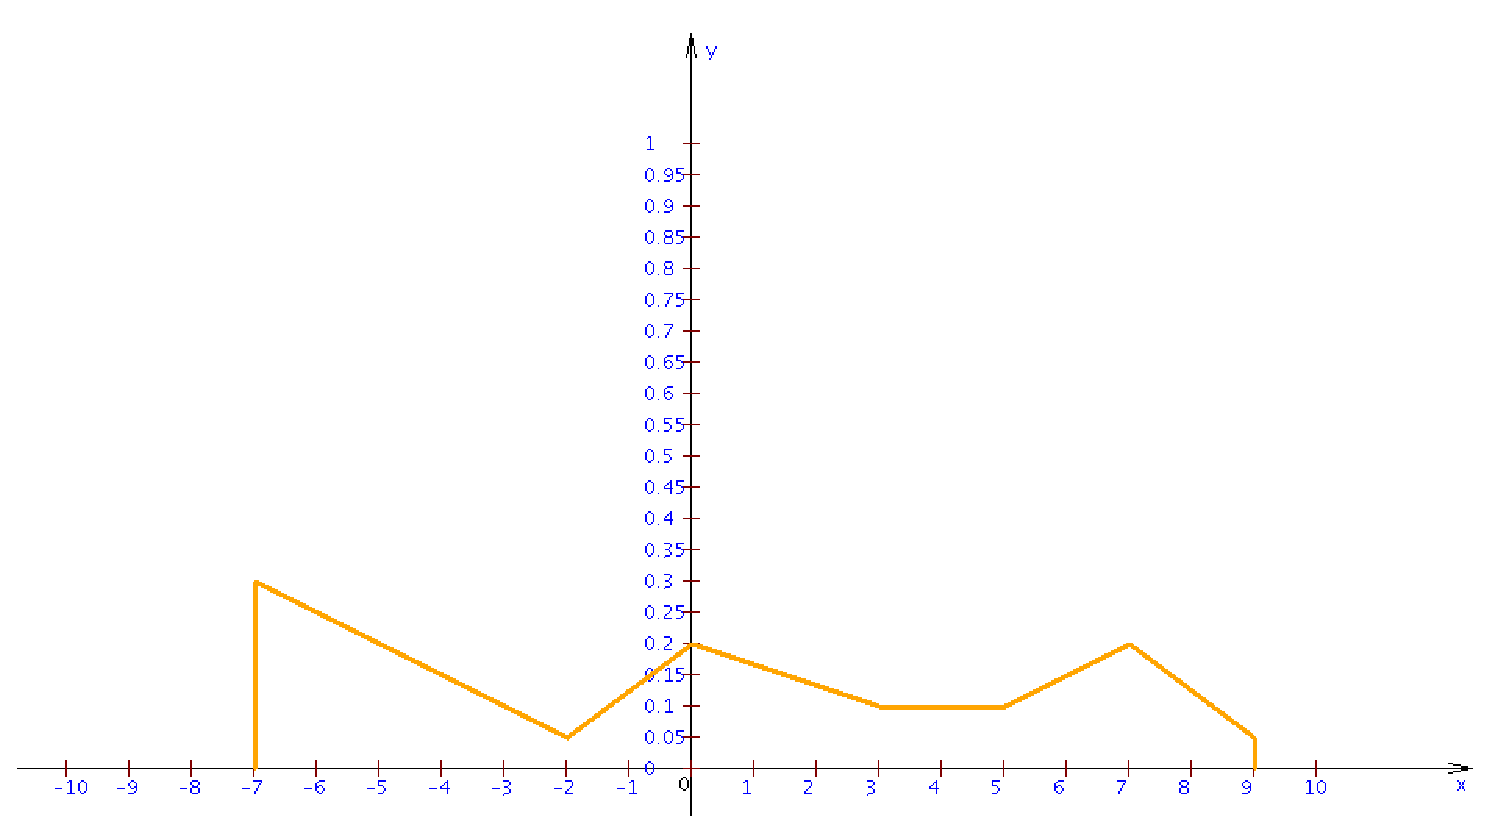
\includegraphics[width=300.57pt, height=192.835pt]{pictures/8_1}
\caption{Polygon of distributions of discrete random variable from the example.
}
\label{8_1}
\end{figure}
%enddelete

\section{Function for sampling}

Function for sampling:

W-matrix of a single line. For example,  $[1, 7, 10, 15]$. 

\comm{sampleMean}{(S)} calculates the sample mean of the sample $S$. 

\comm{sampleDispersion}{(S)} calculates the sample variance of the sample $S$. 

\comm{covarianceCoefficient}{(S1, S2)} calculates the coefficient of covariance for 2 sampling $S1$ and $S2$. 

\comm{correlationCoefficient}{(S1, S2)} calculates the correlation coefficient for 2 sampling $S1$ and $S2$. 

%begindelete
\underline{Example}
%enddelete

\vspace*{-2mm}
\begin{verbatim}
SPACE=R[x, y];
S1=[0, 1]; 
S2=[1, 2];
g=\sampleMean(S1); 
g1=\sampleDispersion(S1); 
g2=\covarianceCoefficient(S1, S2); 
g3=\correlationCoefficient(S1, S2); 
\print(g, g1, g2, g3);
\end{verbatim} 
%begindelete

\ex{$SPACE=R[x, y];$\\
\hspace*{4mm} $S1=[0, 1];$\\ 
\hspace*{4mm} $S2=[1, 2];$\\
\hspace*{4mm} $g=sampleMean(S1); $\\
\hspace*{4mm} $g1=sampleDispersion(S1); $\\
\hspace*{4mm} $g2=covarianceCoefficient(S1, S2); $\\
\hspace*{4mm} $g3=correlationCoefficient(S1, S2);$\\ 
\hspace*{4mm} $print(g, g1, g2, g3);$}
{$g = 0. 5; $\\
\hspace*{4mm} $g1 = 0. 25; $\\
\hspace*{4mm} $g2 = 0. 25; $\\
\hspace*{4mm} $g3 = 1. 00$.} 

%enddelete
 
\chapter{Операторы управления.  Процедурное программирование}

\section{Процедуры и функции}
Система Mathpar позволяет создавать свои процедуры и функции.  Для этого используется команда \comm{procedure}{}.  После команды указывается имя процедуры и в фигурных скобках описывается сама процедура. 

\smallskip

\underline{Пример.}

\vspace*{-3mm}
 
\begin{verbatim}
\procedure myProc2() {
  d = 4;
  \print(d);
}
\procedure myProc(c,  d) {
  if (c < d) {
    \return d;
  } else {
    \return d+5;
  }
}
\myProc2();
a = 10;
c = \myProc(5 + a, a);
\print(a, c);
\end{verbatim}
%begindelete

 Результат выполнения: \\
$d = 4;\  
a = 10;\  
c = 15.$ 
%enddelete

\section{Операторы ветвления и циклов}

 Система Mathpar дает возможность использовать операторы ветвления и циклов. 

\comm{if }{()} \{ \} \comm{else}{} \{ \}~--- оператор ветвления; 

\comm{while }{()} \{ \}~--- оператор цикла с предусловием; 

\comm{for }{(\ ;\ ;\ )} \{ \}~--- оператор цикла с счетчиком.  

\smallskip

\underline{Примеры. }

\vspace*{-3mm}

\begin{verbatim}
a = 5; b = 1;
if (b < a) {
  b = b + a;
} else {
  \print(a, b);
}
if (b < a) {
  b = b + a;
} else {
  \print(a, b);
}
\end{verbatim}
%begindelete

Результат выполнения:\\
$a=5;\ b=6;$

%enddelete
\begin{verbatim}
a = 0;
b = 10;
while (a < b) {
  a = a + 5;
  \print(a);
}
\end{verbatim}
%begindelete

Результат выполнения:\\
$a = 5;$
$a = 10;$

%enddelete
\begin{verbatim}
for (i = 3; i \le 11; i = i + 5) { 
  \print(i);
}
\end{verbatim}

%begindelete
Результат выполнения:\\
$i = 3;$ 
$i = 8.$

\section{Контрольные задания}
В  Mathpar напишите программу:

\begin{itemize}
  \item для поиска наибольшего коэффициента матрицы, 
  \item для вывода всех чисел от 1 до 3000,  которые делятся на 252,  а при делении на 101 дают в остатке 3. 
\end{itemize}
%enddelete

\chapter{Calculations in idempotent algebras}


\section {Tropical algebras}
You can work in the following tropical algebras :

SEMIFIELDS\\
1) On the set of integers $ {\ mathbb Z} $ we define: \\
$ZMaxPlus$,  
$ZMinPlus$.\\
2) On the set of numbers ${\mathbb R}$ we define:\\
$RMaxPlus$, 
$RMinPlus$,  
$RMaxMult$,  
$RMinMult$.\\
3) On the set of numbers ${\mathbb R}64$ we define:\\
$R64MaxPlus$, 
$R64MinPlus$,  
$R64MaxMult$,  
$R64MinMult$.\\

SEMIRINGS\\
1) On the set of numbers ${\mathbb Z}$ we define:\\ 
$ZMaxMin$,
$ZMinMax$,
$ZMaxMult$,
$ZMinMult$.\\
2) On the set of numbers ${\mathbb R}$ we define:\\
$RMaxMin$, 
$RMinMax$.\\
3) On the set of numbers ${\mathbb R}64$ we define:\\
$R64MaxMin$, 
$R64MinMax$.

 

Examples of tropical algebras: 

SPACE = ZMaxPlus [x,  y,  z]; 

SPACE = R64MinMult [u,  v];  

SPACE = RMaxMin [u,  v]. 

 An example of a simple problem in a semiring
 $ZMaxMult$.
%begindelete
\smallskip

\underline{Example 1. }

%\vspace*{-2mm}
%enddelete
\begin{verbatim}
SPACE = ZMaxMult[x, y];
a = 2; b = 9; c = a + b; d = a*b; \print(c, d)
\end{verbatim}
%begindelete

Returns:\\
$c = 9; $\\
$d = 18.$
%enddelete

In the remaining sections of this chapter we have given some examples of problems that are solved in the tropical algebra, which are semi-fields.
%begindelete
\section{Solving systems of linear algebraic equations}
The command $\backslash solveLAETropic(A, b)$ enables us to find a particular solution of the system 
$Ax = b$.
%begindelete
\smallskip

\underline{Example 2. }

%\vspace*{-2mm}
%enddelete
\begin{verbatim}
SPACE = R64MaxPlus[x, y];
A = [
  [1.00, 1.00, 0.00],
  [2.00, 0.00, 3.00],
  [3.00, 4.00, 2.00]
];
b = [8.00, 7.00, 11.00];
X = \solveLAETropic(A, b); 
\print(X);
\end{verbatim}
%begindelete

Returns:\\
$X = \left(\begin{array}{c}
5.00\\
7.00\\
4.00\\
\end{array}\right)
$ 
%enddelete
 
\section{Solving systems of linear algebraic inequalities}
The command $\backslash solveLAITropic(A,b)$ enables us to find a particular solution of the system of inequalities 
%begindelete
\smallskip

\underline{Example 3. }

\vspace*{-3mm}
%enddelete
\begin{verbatim}
SPACE = R64MaxPlus[x, y];
A = [
  [1.00, 1.00, 0.00],
  [2.00, 0.00, 3.00],
  [3.00, 4.00, 2.00]
];
b = [10.00, 7.00, 11.00]; 
X = \solveLAITropic(A, b); 
\print(X);
\end{verbatim}
%begindelete

Returns:\\
$X=[(-\infty,5.00],(-\infty,7.00],(-\infty,4.00]]$ 
%enddelete

%begindelete
\smallskip

\underline{Example 4. }

\vspace*{-3mm}
%enddelete
\begin{verbatim}
SPACE = ZMinPlus[x, y];
A = [
  [1, 1, 0],
  [2, 0, 3],
  [3, 4, 2]
];
b = [10, 7, 11];
X = \solveLAITropic(A, b); 
\print(X);
\end{verbatim}
%begindelete

Returns:\\
$X=[[9,\infty),[9,\infty),[10,\infty)]$ 
%enddelete

\section{The solution of the Bellman equation}
\subsection {The homogeneous  Bellman equation}
The command $\backslash BellmanEquation(A)$ enables us to find a solution of the homogeneous  Bellman equation
  $Ax = x$.
%begindelete
\smallskip

\underline{Example 5.}

\vspace*{-3mm}
%enddelete
\begin{verbatim}
SPACE = R64MaxPlus[x, y];
A = [
  [0.00, -2.00, -\infty, -\infty],
  [-\infty, 0.00, 3.00, -1.00],
  [-1.00, -\infty, 0.00, -4.00],
  [2.00, -\infty, -\infty, 0.00]
]; 
X = \BellmanEquation(A); 
\print(X);
\end{verbatim}
%begindelete

Returns:\\
$$
X=\left(\begin{array}{cccc}
0.00 & -2.00 & 1.00 & -3.00\\
2.00 & 0.00 & 3.00 & -1.00\\
-1.00 & -3.00 & 0.00 & -4.00\\
2.00 & 0.00 & 3.00 & 0.00
\end{array}\right) \left(\begin{array}{c}
v_{1}\\
v_{2}\\
v_{3}\\
v_{4}
\end{array}\right), \forall v_{1}, v_{2}, v_{3}, v_{4}.$$
%enddelete
\subsection {The inhomogeneous  Bellman equation}
The command $\backslash BellmanEquation(A,b)$ enables us to find a solution of the inhomogeneous  Bellman equation $Ax\oplus b=x$.
%begindelete
\smallskip

\underline{Example 6. }

\vspace*{-3mm}
%enddelete
\begin{verbatim}
SPACE = R64MaxPlus[x, y];
A = [
  [0.00, -2.00, -\infty, -\infty],
  [-\infty, 0.00, 3.00, -1.00],
  [-1.00, -\infty, 0.00, -4.00],
  [2.00, -\infty, -\infty, 0.00]
];
b = [[1], [-\infty], [-\infty], [-\infty]]; 
X = \BellmanEquation(A, b); 
\print(X);
\end{verbatim}
%begindelete

Returns:\\
$$X=
 \left(\begin{array}{cccc}
0.00 & -2.00 & 1.00 & -3.00\\
2.00 & 0.00 & 3.00 & -1.00\\
-1.00 & -3.00 & 0.00 & -4.00\\
2.00 & 0.00 & 3.00 & 0.00
\end{array}\right)
\left(\begin{array}{c}
v_{1}\\
v_{2}\\
v_{3}\\
v_{4}
\end{array}\right)
\oplus\left(\begin{array}{c}
1.00\\
3.00\\
0.00\\
3.00
\end{array}\right),$$\\ $$\forall v_{1}, v_{2}, v_{3}, v_{4}.$$
%enddelete
\section{The solution Bellman inequality}
\subsection{The homogeneous Bellman inequality}
 
The command $\backslash BellmanInequality(A)$ enables us to find a solution of the homogeneous Bellman inequality $Ax\leq x$.

\subsection{The inhomogeneous Bellman inequality}
The command $\backslash BellmanInequality(A, b)$ enables us to find a solution of the inhomogeneous Bellman inequality $Ax\oplus b\leq x$.

\section{Finding the shortest path between the vertices of the graph}
\subsection {Calculation of the table of shortest distances for all vertices of the graph}
Let $A=(x_{ij})$ be matrix of distances between adjacent vertices. We put $x_{ii}$=0 $\forall i$ and we put $x_{ij}=\infty$, if there is no edge connecting vertices i and j.
The command $\backslash searchLeastDistances(A)$ allows you to find the smallest distance between all the nodes of the graph.
This results in a matrix of shortest paths between all vertices.
 
%begindelete
\smallskip

\underline{Example 7. }

\vspace*{-3mm}
%enddelete
\begin{verbatim}
SPACE = R64MinPlus[x, y];
A = [
  [0.00, 7.00, 9.00, \infty, \infty, 14.00],
  [7.00, 0.00, 10.00, 15.00, \infty, \infty],
  [9.00, 10.00, 0.00, 11.00, \infty, 2.00],
  [\infty, 15.00, 11.00, 0.00, 6.00, \infty],
  [\infty, \infty, \infty, 6.00, 0.00, 9.00],
  [14.00, \infty, 2.00, \infty, 9.00, 0.00]
];
B = \searchLeastDistances(A);
\print(B);
\end{verbatim}
%begindelete

Returns:\\
$$B= \left(\begin{array}{cccccc}
0.00 & 7.00 & 9.00 & 20.00 & 20.00 & 11.00\\
7.00 & 0.00 & 10.00 & 15.00 & 21.00 & 12.00\\
9.00 & 10.00 & 0.00 & 11.00 & 11.00 & 2.00\\
20.00 & 15.00 & 11.00 & 0.00 & 6.00 & 13.00\\
20.00 & 21.00 & 11.00 & 6.00 & 0.00 & 9.00\\
11.00 & 12.00 & 2.00 & 13.00 & 9.00 & 0.00
\end{array}\right) $$
%enddelete
\subsection {Calculation of the shortest distances between two vertices of the graph}
Let $A=(x_{ij})$ be matrix of distances between adjacent vertices. We put $x_{ii}$=0 $\forall i$ and we put $x_{ij}=\infty$, if there is no edge connecting vertices $i$ and $j$.

The command $\backslash findTheShortestPath(A, i, j)$ allows you to find the shortest path between nodes $i$ and $j$.
 %begindelete
\smallskip

\underline{Example 8. }

\vspace*{-3mm}
%enddelete
\begin{verbatim}
SPACE = R64MinPlus[x, y];
A = [
  [0.00, 7.00, 9.00, \infty, \infty, 14.00],
  [7.00, 0.00, 10.00, 15.00, \infty, \infty],
  [9.00, 10.00, 0.00, 11.00, \infty, 2.00],
  [\infty, 15.00, 11.00, 0.00, 6.00, \infty],
  [\infty, \infty, \infty, 6.00, 0.00, 9.00],
  [14.00, \infty, 2.00, \infty, 9.00, 0.00]
];
X = \findTheShortestPath(A, 0, 4);
\print(X);
\end{verbatim}
%begindelete

Returns:\\
$X=[[0, 2, 5, 4]]$
%enddelete
 

\chapter{The calculations on a supercomputer}
In order to solve computational problems that require large computation time or large amounts of memory, the system has special functions that provide the user with resources of
supercomputer. These functions allow you to perform calculations on a dedicated set of cores. The number of kernels ordered by the user.

You have the following functions ( {\it 3ar-functions}) that apply to supercomputer:

1) \comm{matMultPar1x8}{}~--- calculation of the matrix product;

2) \comm{adjointDetPar}{}~--- computation of the adjoint matrix and determinant;

3) \comm{charPolPar}{}~--- computation of the characteristic polynomial of a matrix;

4) \comm{polMultPar}{}~--- computation of the product of two polynomials;

5) \comm{BellmanEquationPar}{A}~---  solution of a homogeneous Bellman equation  $Ax=x$;

6) \comm{BellmanEquationPar}{A,b}~--- solution of an inhomogeneous Bellman equation   $Ax+b=x$;

7) \comm{BellmanInequalityPar}{A}~--- solution of a homogeneous Bellman  inequality $Ax\leq x$;

8) \comm{BellmanInequalityPar}{A,b}~--- solution of an inhomogeneous Bellman  inequality $Ax+b\leq x$; 

 
%1) \comm{gbasisPar}{}~--- computation of Grobner basis;

%2) \comm{adjointPar}{}~--- computation of the adjoint matrix;

%3) \comm{adjointDetPar}{}~--- computation of the adjoint matrix and determinant of the matrix;

%4) \comm{echelonFormPar}{}~--- computation of the matrix echelon form;

%%5) \comm{inversePar}{}~--- computation of the inverse matrix;

%6) \comm{detPar}{}~--- computation of the determinant of the matrix;

%7) \comm{kernelPar}{}~--- computation of the kernel of a linear operator;

 
 
Before applying any of these functions, the user must specify the parameters that define the parallel environment:

$ TOTALNODES $~--- total number of processors (cores), which provides for the computation

$ PROCPERNODE $~--- number of cores on a single node,

$ CLUSTERTIME $~--- maximum time (in minutes) execution of the program, after which the program is forced to end. 

$MAXCLUSTERMEMORY$~--- amount of memory allocated for the JVM for a one  process (for -Xmx parameter).

To set the number of cores on a single node the user must know what a cluster is used and how many cores it is available on the node. By default, the $ TOTALPROCNUMBER $ and $ NODEPROCNUMBER $ installed so that all the cores were used per node, and $ CLUSTERTIME = 1 $.

The user can change the number of cores on a single node. This is an important feature, since the memory on a single node is used by all $ NODEPROCNUMBER $ cores. Consequently, the user can regulate the size of of RAM that is available to one core.

\section{Parallel polynomial computations}
   For parallel computation  of the  polynomial product you can use the 
   \comm{multiplyPar}{(p1, p2)}, where $ p1 $, $ p2 $~--- given polynomials.

\underline{Example. }
\begin{verbatim}
TOTALNODES=2; 
PROCPERNODE=1;
CLUSTERTIME=1; 
f=x^2+3y;
g=x^2+3y+3z;
\polMultPar(f,g);
\end{verbatim}

%%  For parallel computing Grobner basis you must use the 
%  \comm{gbasisPar}{([p1, p2, p3,\ldots, pn])}, where $p1, p2, p3,\ldots, pn$~--- polynomials. 
%\underline{Example. }
%\begin{verbatim}      
%\gbasisPar([x^2+2x+1, x^4+x-2]); 
%\end{verbatim}
      
\section{Parallel matrix computations}
  For parallel computing  products of matrices $ m1 $ and $ m2 $   you must use the 
  \comm{multiplyPar}{(m1, m2)}. 
 
  \underline{Example. }
\begin{verbatim}
TOTALNODES = 2;
PROCPERNODE = 1;
A=[[0,1],[2,3]];
B=[[5,61],[7,8]];
\matMultPar1x8(A, B);
\end{verbatim}


  For parallel computation of the adjoint matrix for the matrix $ m $ you can use the 
  \comm{adjointPar}{(m)}.  
 
  Similarly, for the matrix $ m $ you can perform the calculation of the echelon form \comm{echelonFormPar}{(m)}, the computation of the determinant \comm{detPar}{(m)},
computation of the kernel \comm{kernelPar}{(m)}, the calculation of the characteristic polynomial \comm{charPolPar}{(m)}. The command \comm{adjointDetPar}{(m)}
allows us to calculate the determinant and adjoint matrix simultaneously.

   \underline{Example. }
\begin{verbatim}
TOTALNODES = 2;
PROCPERNODE = 1;
SPACE = Z[x];
A=[[0,1],[2,3]];   
\adjointDetPar(A);
\end{verbatim}

\ section {Running your parallel programs}
Mathpar allows you to download and execute your parallel programs.
Your package must be in the root directory of the project.
To ensure that your program is able to interact with the system management tasks, 
you need to add an initialization string 

{\bf QueryResult queryRes = Tools.getDataFromClusterRootNode (args)}

\noindent
 (immediately after MPI.Init) and the completion string 

{\bf Tools.sendFinishMessage (args)}

\noindent
 (before MPI.Finalize) in your main-method.
You can also pass any arguments to your program from the web-interface Mathpartner. 
Within the program you can get them by calling queryRes.getData (). Below is an example of a 
parallel program that simply outputs on standard output the arguments passed to it.

\begin{verbatim}
        MPI.Init(args);
        QueryResult queryRes=Tools.getDataFromClusterRootNode(args);
        int myRank=MPI.COMM_WORLD.getRank();
        if (myRank == 0) {
            Object []ar=queryRes.getData();
            System.out.println("test...");           
            for (int i=0; i<ar.length; i++){
                System.out.println(((Element)ar[i]).intValue());
            }            
        }
        Tools.sendFinishMessage(args);
        MPI.Finalize();
\end{verbatim}

After that you need to compile the program, and the program folder packed in zip-archive.Then you need to download this file to the server, using the tab "File" and clicking "download file".
 
RAM is divided equally between all cores. For example, if the cluster node has 8GB of memory,
then if you request 4 cores on a single processor, each will receive 2GB, 
and if you have requested one core - then it will get 8GB.

The command to download your zip-archive, which contains java-classes, as follows:

\comm{uploadToCluster} {(FileName)}, where FileName - name of zip-archive.

To view a list of all your downloaded files on a cluster, use the command

\comm{showFileList} {()}.

To run your program, use the command

\comm {runUploadedClass} {(archieveName, classPath, param0, param1, ...)},
where 
{\bf archieveName} - the name of the downloaded zip-archive with the program, 
{\bf classPath} - the path to the class containing main-method (full path with the packages)
{\bf paramX} - arbitrary parameters specified separated by commas, to be passed to your program.

To monitor the running programs, use the command

\comm {getStatus} {(taskID)}

It is also possible to get a list of all the tasks of the current user with a 
description of their states:

\comm {showTaskList} {()}

To receive the content from the output stream and error stream, use the commands

\comm {getOut} {(taskID)}

\comm {getErr} {(taskID)}

Files that contain output or error stored on a cluster of two days,
zip-archives containing the compiled java-classes are stored for 30 days.
\chapter{Operators and mathematical symbols} 

{\bf Naming rules for Mathematical Objects}

\bigskip
 
Uppercase and lowercase letters are different everywhere. The user can give any names for mathematical objects. However, these names should not coincide with the operators and constants that are defined in the system. In addition, the names of objects, of which the multiplication is not commutative, for example, vectors and matrices, must begin with a capital Latin letters, and all other object names must start with lowercase letters. This makes it possible as soon as entering automatically get a simplified expression.
\bigskip

Here is a list of the main operators of the system Mathpar.   


\comm{clean}{}~---  clean input data (if this operator doesn't have arguments) or the date of arguments of this operator,

\bigskip

{\bf Infix arithmetic operators}


{\bf +}~---  addition; 

{\bf -}~---  subtraction; 

{\bf /}~---  division;

{\bf *}~---  multiplication (still a blank or absence of the operator);

\comm{times}{}~--- noncommutative multiplication(still a blank or absence of the operator);  

\bigskip

\bigskip

{\bf Postfix arithmetic operators}

{\bf !}~---  factorial;

{ ${x} \widehat{\ }{\{ \}}$}~---  exponentiation;
\bigskip

{\bf Comparisons} 

$\mathbf{\backslash le}$~---  less than or equal;

${\mathbf >}$~---  it is more; 

$\mathbf{\backslash ge}$~--- it is more or equally; 

{\bf ==}~---  it is equal; 

$\mathbf{\backslash ne}$~--- it is unequal;  
\bigskip

{\bf Infix Boolean operators}


 $\mathbf{ \backslash lor}$ ~--- disjunction (logic OR); 

 $\mathbf{  \backslash \&}$~--- conjunction (logic AND); 

$\mathbf{ \backslash neg}$ ~--- negation.  


{\bf Key prefix operators}

 \comm{d}{}~--- the symbol of derivative, wich is usualy used in the differential equations,

 \comm{D}{}~--- the operator of differentiation: \comm{D}{(f)} and \comm{D}{(f, x)} are the first derivative by $x$; \comm{D}{(f, y{\ }\widehat{\ }\ 3)} is the third derivative by $y$;

 \comm{expand}{}~--- opening all brackets;

 \comm{fullExpand}{}~--- to expand expression containing logarithmic, exponential and trigonometric  functions;

 \comm{extendedGCD}{}~--- extended polynomial GCD, returns a vector containing GCD and additional multipliers of arguments;

  \comm{GCD}{}~--- GCD of polynomials; 

 \comm{factor}{}~--- to factor expression;  

 \comm{fullFactor}{}~--- to factor expression containing logarithmic and exponent functions;

 \comm{initCond}{}~--- boundary conditions for a system of linear differential equations;

 \comm{LCM}{}~--- polynomial LCM; 

 \comm{lim}{}~--- the sign for limit; 

 \comm{print}{}~--- the print operator of the expressions, the names of which are listed in this operator (each expression printed in the new line);

 \comm{printS}{}~--- the print operator, which is similar to the Pascal print operator(for printing in several lines you can use the symbol ``$\backslash$n'';
 
 \comm{plot}{}~--- to plot explicit functions; 
 
  \comm{plot3D}{}~--- to plot functions of two variables, which are given explicitly;

 \comm{paramPlot}{}~--- to plot parametric functions;  

\comm{tablePlot}{}~--- to plot of function, which are presented by the table of arguments and values; 

 \comm{prod}{}~--- the symbol of product ($\prod$); 

 \comm{randomPolynom}{}~--- to generate a random polynomial; 

 \comm{randomMatrix}{}~--- to generate a random matrix; 

 \comm{randomNumber}{}~--- to generate a random number; 

 \comm{sequence}{}~--- the sequence; 

 \comm{showPlots}{}~--- to display at one field of schedules of functions of different types;
 
 \comm{solveLDE}{}~--- to solve system of the linear differential equations; 

 \comm{systLAE}{}~--- to set the system of the linear algebraic equations; 

 \comm{systLDE}{}~--- to set the system of the linear differential equations; 

 \comm{sum}{}~---  a summation symbol ($\sum$); 

 \comm{time}{}~--- this operator returns the processor time in milliseconds;  

 \comm{value}{}~--- to calculate value of expression by means of substitution of the expressions (or numbers) instead of ring variables; 
 
\bigskip
 
 {\bf Operators of the procedure, branching and loop}

 \comm{procedure}{}~--- ad procedures;
 
\comm{if }{(\ ) \{\  \}} \comm{else }{\{ \ \}}~--- operator of the branch;

\comm{while }{( \ ) \{ \ \}}~--- operator of the cycle with a precondition;

\comm{for }{(\ ; \ ; \ ) \{ \ \}}~--- cycle operator with a counter. 

\bigskip

{\bf Matrix, matrix elements and  matrix operators}

[\ , \  ] ~--- setting vector (row-vector);

[[\ ,\  ], [\ ,\  ]]~--- the matrix may be defined as vector of vectors;  


A\_\{i,j\}~--- (i,j)-element of the matrix A;

A\_\{i,?\}~---  row i of the matrix A;

A\_\{?,j\}~---  j column of the matrix A;

$\backslash$IO\_\{n,m\}~--- zero matrix of size $ n \times m $;

$\backslash$I\_\{n,m\}~---  $n \times m$  matrix with ones on the diagonal;

+, -, *~--- addition, subtraction, multiplication; 

\comm{charPolynom}{}~---  calculation of a characteristic polynomial; 
 
\comm{kernel}{}~--- calculation of a kernel (zero-space of matrix); 

\comm{transpose}{} or  $\mathbf{A \widehat{\ } \{T\}}$~--- transposing;  
 
\comm{conjugate}{} or  $\mathbf{A\widehat{\ }\{\backslash ast\}}$~--- conjugate;

\comm{toEchelonForm}{}~---   calculation of the matrix echelon form;  

\comm{det}{}~---   calculation the determinant; 
 
\comm{inverse}{}  or  $\mathbf{A}\widehat{\ }\{-1\}$~---  calculation of the inverse matrix; 

\comm{adjoint}{}  or  $\mathbf{A}\widehat{\ }\{\backslash star\}$~--- calculation of the adjoint matrix;  
 
\comm{genInverse}{}  or $\mathbf{A}\widehat{\ }\{+\}$~--- generalized inverse matrix Murr-Penrose;
 
\comm{closure}{}   or $\mathbf{A}\widehat{\ }\{\backslash times\}$~--- closure, i.e. the amount of 
$ I + A + A^2 + A^3 + \ldots $. 
For the classical algebras is equivalent to $ (I-A)^{-1} $.

\comm{LDU}{}~--- LDU-decomposition of matrix. The result is a vector of three matrices [L,D,U]. Where L is a lower triangular matrix, U~--- upper triangular matrix, 
D~--- permutation matrix, multiplied by the inverse of the diagonal matrix. 

\comm{BruhatDecomposition}{}~--- Bruhat decomposition of matrix. The result is a vector of three matrices [V,D,U]. Where V and U~--- upper triangular matrices, 
D~--- permutation matrix, multiplied by the inverse of the diagonal matrix.

  

\chapter{Примеры решения задач по физике}
\section{Передача тепла}

\begin{verbatim}
"ЗАДАЧА 1"
"Кусок льда массой"
M = 10 кг;
"помещен в сосуд. Температура льда"
T = -10  \degreeC ;
"Найдите массу воды в сосуде после того, как сосуду 
сообщили количество тепла равное"
q = 20000 кДж;
"Удельная теплоемкость воды"
c_v = 4.2 кДж/(кг \degreeC);
"Удельная теплоемкость льда"
c_i = 2.1 кДж/(кг \degreeC);
"Удельная теплота плавления льда"
r = 330 кДж/кг;
"Удельная теплота испарения воды"
\lambda = 2300 кДж/кг;
END
\end{verbatim}

\vspace*{3mm}

\begin{verbatim}
"РЕШЕНИЕ ЗАДАЧИ 1"
"Искомую массу воды обозначим через x."
SPACE = R64[x];
"Обозначим количество теплоты требуемое для нагревания льда до 0 градусов:"
q_1 = M c_i (0 - T);
"для плавления всего льда:"
q_2 = M r;
"для нагревания воды до ста градусов:"
q_3 = M c_v (100 \degreeC);
"для испарения части воды"
q_4 = (M - x)\lambda;
"Здесь мы обозначили через x массу оствшейся в сосуде воды."
"По условию задачи должно выполняться равенство,
решая которое найдем неизвестное x:"
mass  = \solve (q = q_1 + q_2 + q_3 + q_4);
mass=\value(mass);
\print(mass);
\end{verbatim}
\vspace*{-3mm}
 


\section{Кинематика} 

\begin{verbatim}
"ЗАДАЧА 2"
"Кинематическое уравнение движения точки по прямой (по оси x) 
имеет вид $x = c_1 + c_2 t + c_3 t^3$."
"Найдите: (1) координату точки, (2) мгновенную скорость,
(3) мгновенное ускорение" 
END
\end{verbatim}\vspace*{-3mm}
 
 \
 
\begin{verbatim}
"РЕШЕНИЕ ЗАДАЧИ 2."
"Выбираем пространство с переменными $t, c_1, c_2, c_3$:"
SPACE = R64[t, c_1, c_2, c_3];
"Уравнение движения точки"
x = c_1 + c_2  t + c_3 t^3;
"Вычислим мгновенную срость"
v = \D_t(x);
"Вычислим мгновенное ускорение"
a = \D_t(v);
\print(x, v, a);
\end{verbatim}\vspace*{-3mm}

\

\begin{verbatim}
"ЗАДАЧА 2А"
"Решите предыдущую задачу, при условии, что  "
"коэффициенты c1, c2, c3 в уравнении имеют следующие значения"
Coeff = [4, 2, -0.5];
"и момент времени равен "
t_0 = 2 "секунды." 
END
\end{verbatim}\vspace*{-3mm}

\

\begin{verbatim}
"РЕШЕНИЕ ЗАДАЧИ 2А"
"Введем обозначение для элементов вектора  Coeff:"
cf=\elementOf(Coeff);
"Найдем числовое значение каждой функции (x, v, a)
в точке"
arg = [t_0, cf_{1}, cf_{2}, cf_{3}];
"(1) координата точки в момент времени $t_0$:"
x_0 = \value (x, arg);
"(2) мгновенная скорость точки в момент времени $t_0$:"
v_0 = \value (v, arg);
"(3) мгновенное ускорение точки в момент времени $t_0$:"
a_0 = \value (a, arg);
\print(x_0, v_0, a_0);
\end{verbatim}\vspace*{-3mm}

\

\section{Молекулярная физика} 
 
 \
 
\begin{verbatim}
"ЗАДАЧА 3"
"В центре горизонтальной трубки расположен столбик ртути длиной h" 
"Часть воздуха была выкачана и концы трубки запаяны.   
Трубка имеет длину l" 
"Когда трубка была поставлена вертикально, столбик ртути переместился вниз на расстояние $l_d$." 
"Ускорение свободного падения обозначим $g$, плотность ртути — $\rho$"
"Какое начальное давление было в трубке?"
END
\end{verbatim}\vspace*{-3mm}

\

\begin{verbatim}
"РЕШЕНИЕ ЗАДАЧИ 3"
"Пусть в трубке было начальное давление $p_0$. Введем пространство с переменной $p_0$:"
SPACE=R64[p_0];
"После поворота трубки давление в нижней части трубки повысилось, 
так как добавилось давление столбика ртути. Следовательно, новое давление стало равно:" 
p_1 = p_0+\rho g h; 
"Пусть s это площадь поперечного сечения трубки. 
Тогда начальный обьем нижней части трубки равен:"
v_0=  (l/2-h/2) s; 
" После поворота трубки обьем воздуха в нижней части трубки будет  равен:"
v_1=  (l/2-h/2-l_d) s;
"В соответствии с законом Бойля-Мариотта запишем и решим 
уравнение относительно неизвестной $p_0$:"
initialPressure = \solve(p_0 v_0=p_1 v_1 );
\print(initialPressure );
\end{verbatim}

\

\begin{verbatim}
"ЗАДАЧА 3А."
"Решите предыдущую задачу предполагая, что переменные 
имеют следующие числовые значения: "
h = 0.20 m;
l = 1 m;
l_d = 0.10 m;
g = 9.8 m/s^2;
\rho = 13600 kg/m^3;
END
\end{verbatim}

\

\begin{verbatim}
"РЕШЕНИЕ ЗАДАЧИ 3А"
p_1 = p_0 + \rho g h;
v_0 = (l/2 - h/2) S; 
v_1 = (l/2 - h/2 - l_d) S;
\solve(p_0 v_0 = p_1 v_1);
\end{verbatim}

\vfill
\thispagestyle{empty}
\end{document}
